\documentclass[11pt,class=report,crop=false]{standalone}
\usepackage[screen]{../mathgame}


\begin{document}


%====================================================================
\chapitre{Approximation et interpolation}
%====================================================================

%
%\insertvideo{yUgpElITYTg}{partie 5.1. Bits classiques}
%
%\insertvideo{iET0snUXj0k}{partie 5.2. Portes logiques}
%
%\insertvideo{JKmC2u5kvKg}{partie 5.3. Algorithme et complexité}



\objectifs{L'approximation a pour but de modéliser une situation à l'aide d'une fonction simple. 
Avec une fonction simple, les calculs sont plus rapides. L'interpolation modélise des données partielles par une fonction. 
On obtient ainsi une fonction qui permet de prédire des valeurs manquantes.}

%%%%%%%%%%%%%%%%%%%%%%%%%%%%%%%%%%%%%%%%%%%%%%%%%%%%%%%%%%%%%%%%%%%%%
\section{Approximation locale}

\index{approximation!developpement limite@développement limité}

%--------------------------------------------------------------------
\subsection{Développement limité à l'ordre 1}

On considère une fonction $f : I \to \Rr$ dérivable autant de fois que nécessaire sur un intervalle $I \subset \Rr$.
Fixons un point $x_0 \in I$. Comme $f$ est continue alors $f(x) \simeq f(x_0)$ pour tout $x$ proche de $x_0$.
Comment obtenir une meilleure approximation ?
On va utiliser la dérivée pour écrire un développement limité à l'ordre de $1$ de $f$ autour de $x_0$ :
\mybox{$f(x) \simeq f(x_0) + (x-x_0) f'(x_0)$}

En écrivant $x = x_0+h$ (avec $h$ proche de $0$ lorsque $x$ est proche de $x_0$), une autre écriture possible est :
\mybox{$f(x_0+h) \simeq f(x_0) + h f'(x_0)$}

Géométriquement cela correspond à approcher le graphe de $f$ autour de $x_0$ par la tangente à ce graphe en $x_0$. Bien sûr, un développement limité 
ne fournit qu'une approximation locale qui n'a aucune utilité si $x$ est trop éloigné de $x_0$.

\begin{exemple}
Considérons $f(x) = \frac{1}{\sqrt{x}}$ autour de $x_0 = 1$. 
On a $f'(x) = -\frac{1}{2x\sqrt{x}}$. Ainsi $f(x_0) = 1$ et $f'(x_0) = -\frac{1}{2}$. Le DL de $f$ d'ordre $1$ autour de $x_0 = 1$ est :
$$\frac{1}{\sqrt{x}} \simeq 1 - \frac{1}{2}(x-1)$$
ou encore :
$$\frac{1}{\sqrt{1+h}} \simeq 1 - \frac{1}{2}h.$$



Combien vaut $\frac{1}{\sqrt{1.1}}$ ? Avec $h=0.1$, on obtient $\frac{1}{\sqrt{1.1}} \simeq 0.95$. 
Ce qui est proche de la valeur exacte $\frac{1}{\sqrt{1.1}} = 0.953463\ldots$ 

Sur le dessin de gauche ci-dessous est tracée la courbe de $f$, ainsi que son DL d'ordre $1$ (c'est donc la tangente à la courbe en $x_0=1$). 
Sur la figure de droite on mesure l'erreur commise par le DL d'ordre $1$, c'est-à-dire le graphe de $f(x)- (1 - \frac{1}{2}(x-1))$.

\begin{center}
  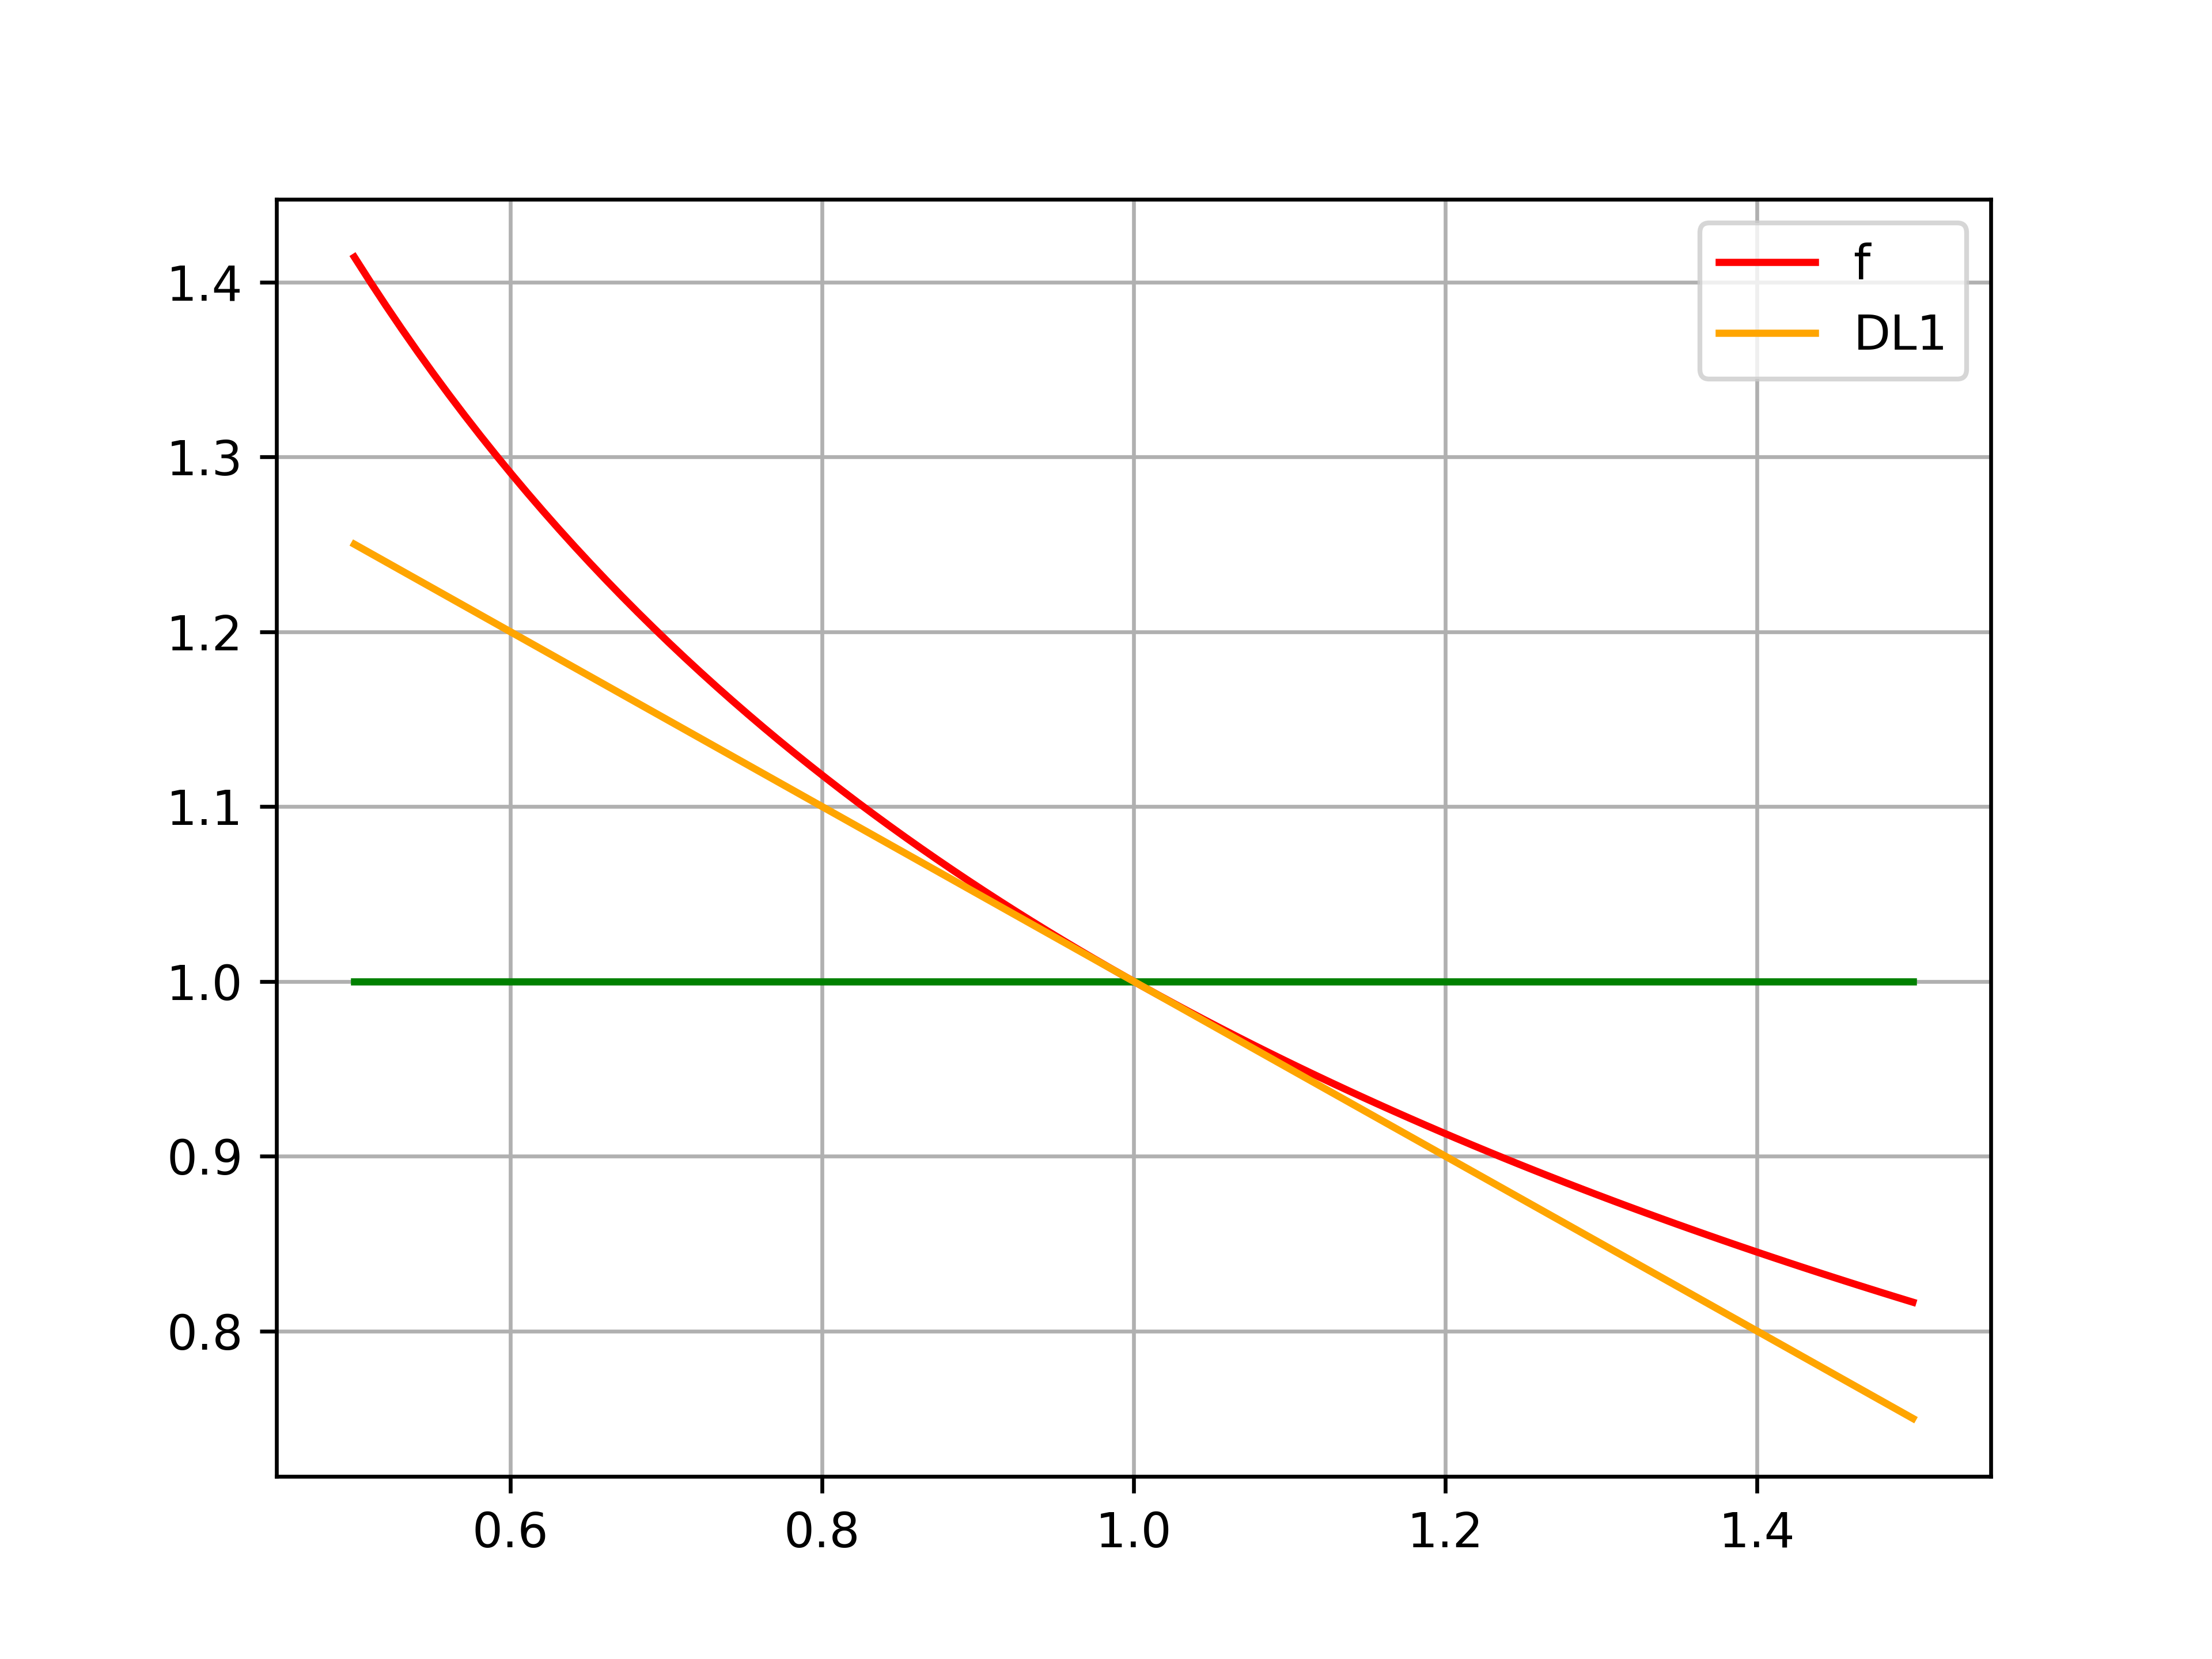
\includegraphics[scale=\myscale,scale=0.5]{figures/approx-dl-01}
  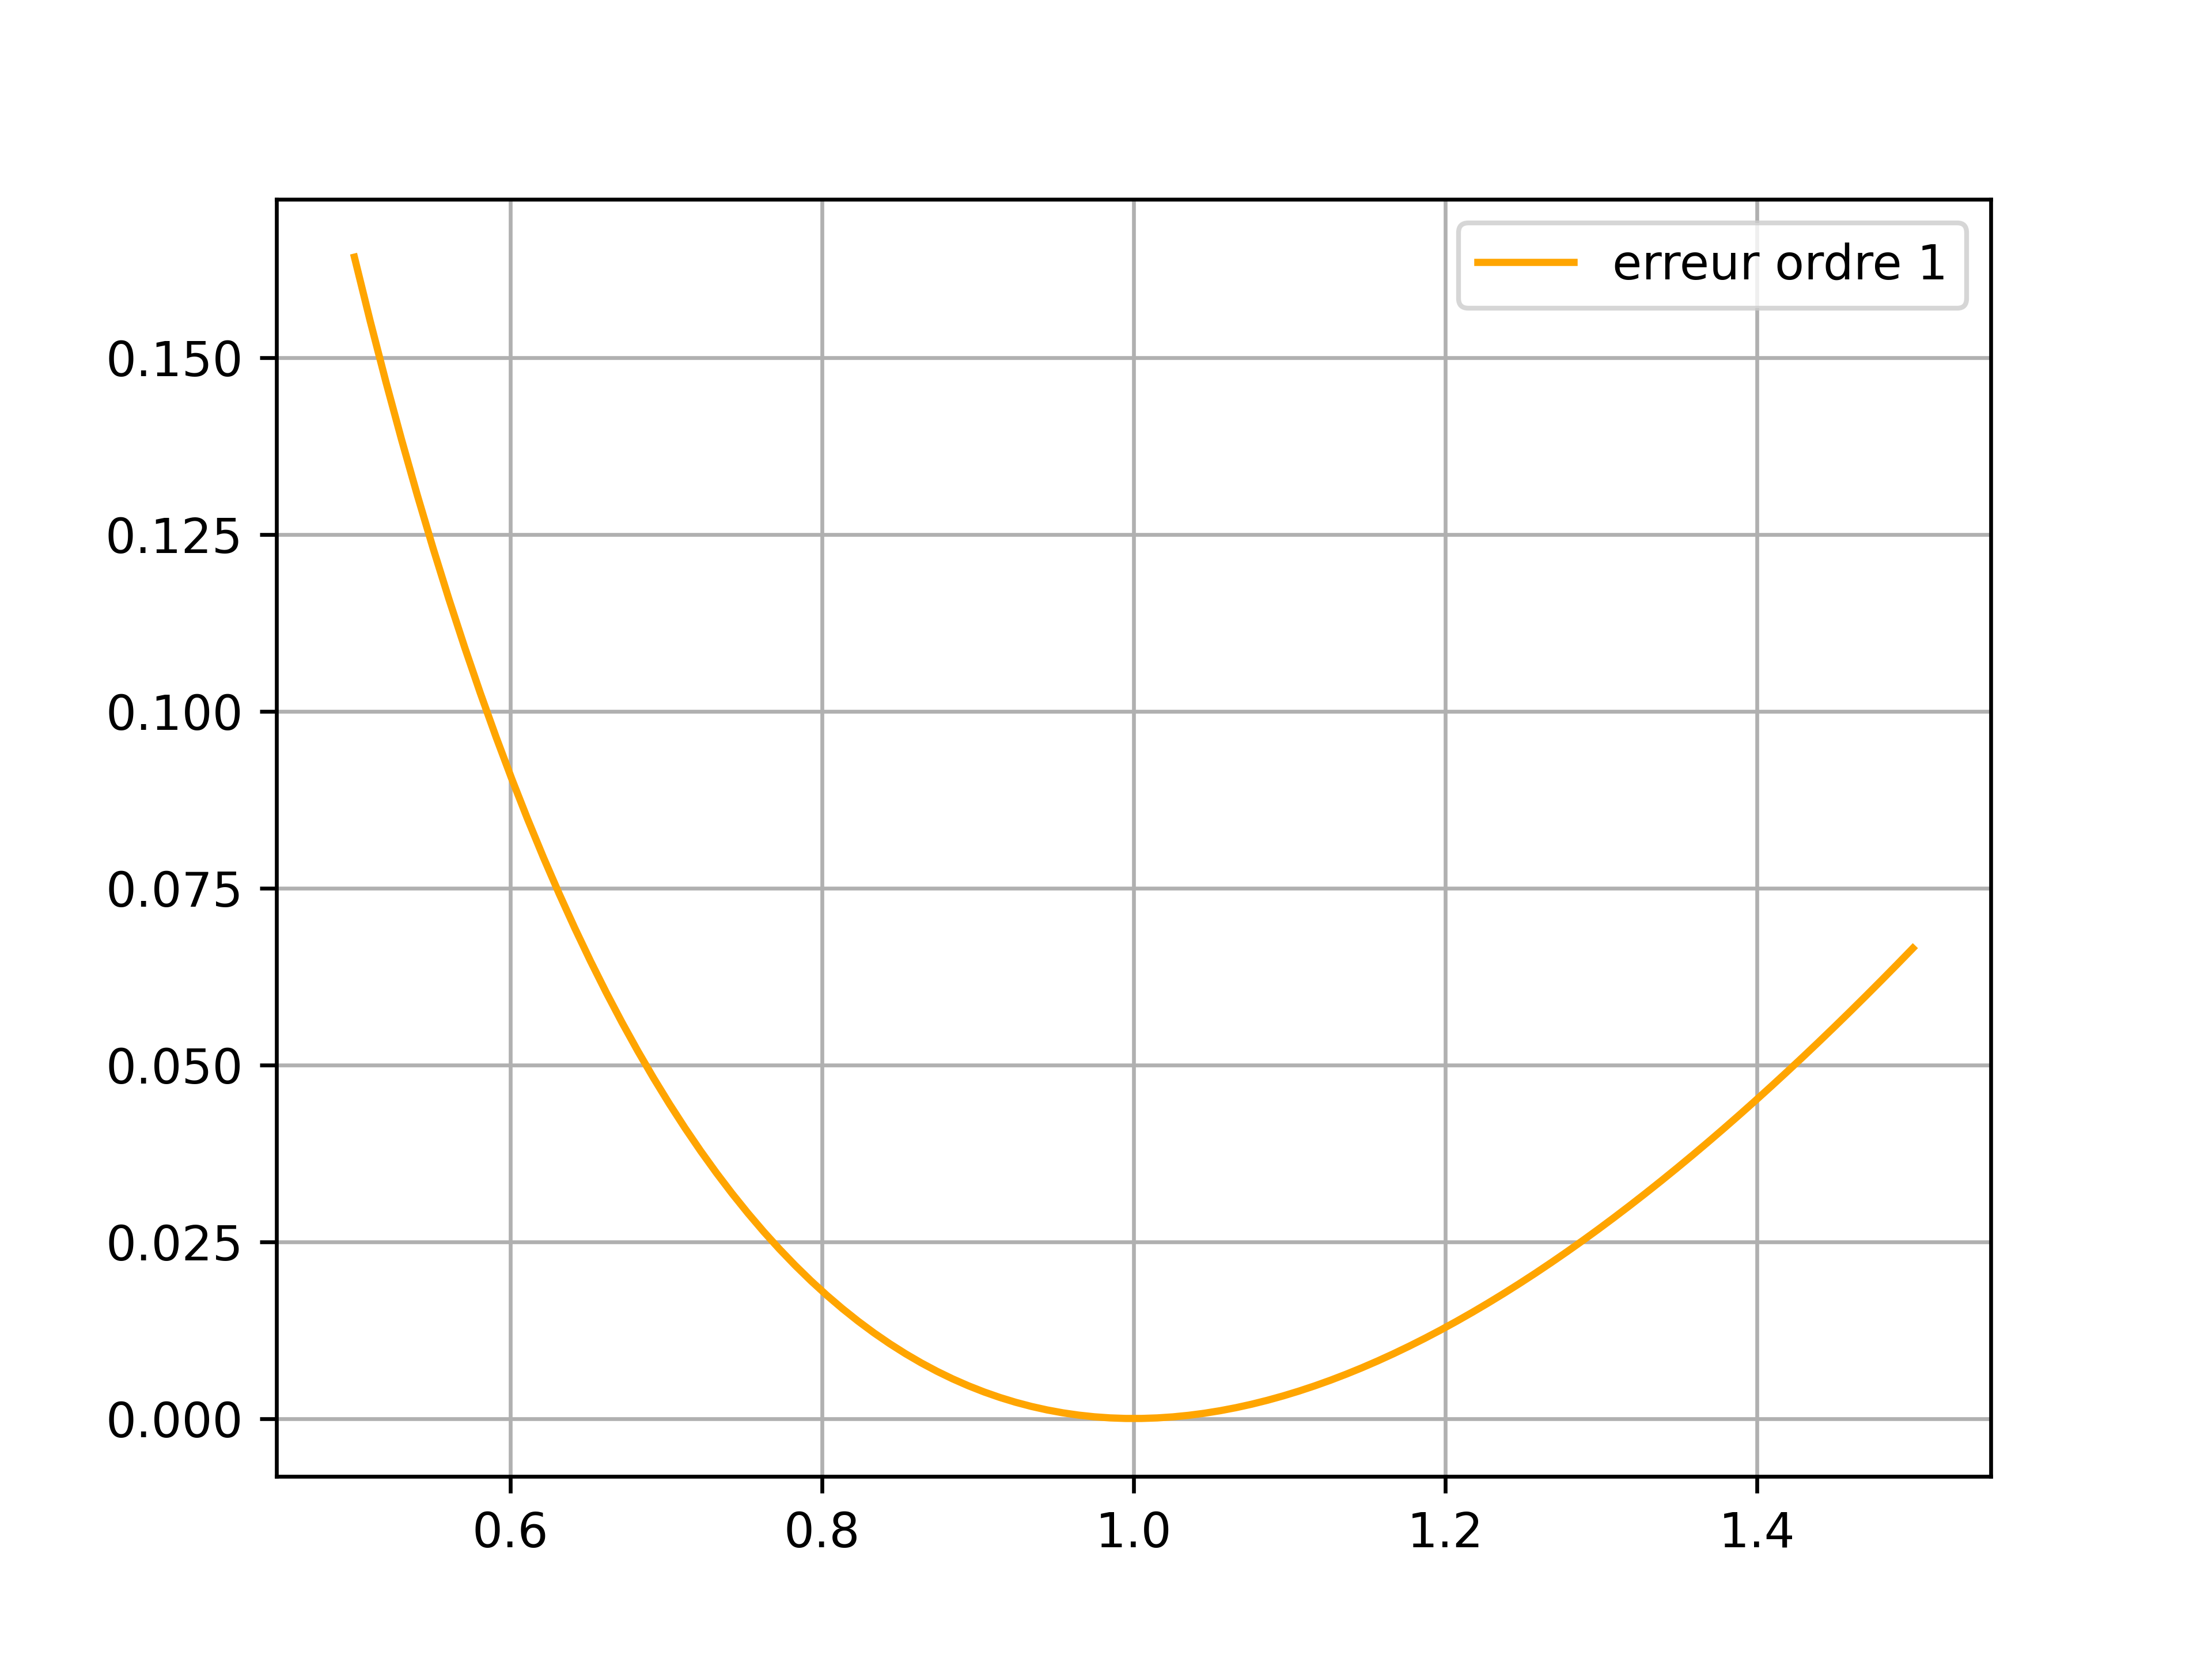
\includegraphics[scale=\myscale,scale=0.5]{figures/approx-dl-02} 
\end{center}

\end{exemple}

\textbf{Normalisation.} Le calcul de $\frac{1}{\sqrt{x}}$ est particulièrement important car il est utilisé dans la normalisation d'un vecteur.
Par exemple : comment trouver le point $P$ situé à une distance $t$ du point $S$ dans la direction du vecteur $\vec{v}$ ?
C'est le point :
$$P = S + t \frac{\vec{v}}{\|\vec{v}\|}$$

\myfigure{1}{
	\tikzinput{fig-approx-01}
}  

Si $\vec{v} = (v_x, v_y)$ alors $\frac{\vec{v}}{\|\vec{v}\|} = \frac{1}{\sqrt{v_x^2 + v_y^2}} (v_x, v_y)$.
Les calculs de $\frac{1}{\sqrt{x}}$ sont désormais directement implémentés dans les processeurs graphiques.
Noter que notre approximation par un DL d'ordre $1$ n'est valide que pour des vecteurs qui sont déjà proches d'une norme $1$.
Une autre technique consiste à appliquer la méthode de Newton, également basée sur la dérivée ; avec un choix judicieux de la valeur initiale, une seule itération peut suffire (\og{}astuce de Carmack\fg{}).



%--------------------------------------------------------------------
\subsection{Développement limité à l'ordre $n$}

Voici la formule du DL de $f$ en $x_0$ à l'ordre $n$ :
\mybox{$\displaystyle
f(x) \simeq f(x_0)+f'(x_0)(x-x_0)+\frac{f''(x_0)}{2!}(x-x_0)^2 +\cdots +\frac{f^{(n)}(x_0)}{n!}(x-x_0)^n
$}

Ce que l'on peut récrire :
$$f(x_0+h) \simeq f(x_0)+f'(x_0)h+\frac{f''(x_0)}{2!}h^2+\cdots
+\frac{f^{(n)}(x_0)}{n!}h^n$$
c'est-à-dire :
$$f(x_0+h) \simeq \sum_{k=0}^n \frac{f^{(k)}(x_0)}{k!}h^k.$$

Géométriquement un DL à l'ordre $2$ correspond à approcher le graphe de $f$ par une parabole autour de $x_0$.
Un DL à l'ordre $n$ correspond à approcher le graphe de $f$ par une courbe polynomiale de degré $n$ autour de $x_0$.
Plus $n$ est grand, plus la courbe polynomiale est proche du graphe de $f$, mais toujours seulement autour de $x_0$.



\begin{exemple}
Considérons $f(x) = \frac{1}{\sqrt{x}}= x^{-\frac12}$ autour de $x_0 = 1$.
On a $f'(x) = -\frac{1}{2}x^{-\frac32}$ et $f''(x) = \frac34 x^{-\frac52}$ et $f'''(x) = -\frac{15}{8}{x^{-\frac72}}$
ce qui permet de calculer les coefficients $\frac{f^{(k)}(x_0)}{k!}$.
Les DL à l'ordre $1$, $2$ et $3$ donnent donc :
$$\frac{1}{\sqrt{1+h}} \simeq 1 - \frac{1}{2}h$$
$$\frac{1}{\sqrt{1+h}} \simeq 1 - \frac{1}{2}h + \frac{3}{8}h^2$$
$$\frac{1}{\sqrt{1+h}} \simeq 1 - \frac{1}{2}h + \frac{3}{8}h^2 - \frac{5}{16}h^3$$

Avec $h=0.1$ on obtient $\frac{1}{\sqrt{1.1}} \simeq 0.953437$ via le DL à l'ordre $3$, ce qui donne $4$ chiffres exacts après la virgule.
\end{exemple}

\begin{exemple}
On souhaite approcher $f(x) = \sin(x)$ par un polynôme sur l'intervalle $[0, \frac\pi2]$.

\textbf{DL en $0$.}
En posant $x_0 = 0$, on a $f(0) = 0$, $f'(0) = 1$, $f''(0) = 0$ et $f'''(0) = -1$.
Le DL à l'ordre $3$ en $0$ est donc :
$$\sin(x) \simeq x - \frac{1}{6}x^3$$

\textbf{DL en $\frac\pi4$.}
En posant $x_0 = \frac\pi4$, on calcule $f(\frac\pi4) = \frac{1}{\sqrt2}$, $f'(\frac\pi4) = \frac{1}{\sqrt2}$,\ldots
Le DL à l'ordre $3$ en $\frac\pi4$ est donc :
$$\sin(x) \simeq \frac{1}{\sqrt2} + \frac{1}{\sqrt2}\left(x-\frac\pi4\right) - \frac{1}{2\sqrt2}\left(x-\frac\pi4\right)^2 - \frac{1}{6\sqrt2}\left(x-\frac\pi4\right)^3$$

\textbf{Comparaison.}
Sur $[0,\frac\pi2]$ le DL en $\frac{\pi}{4}$ est plus précis que le DL en $0$ car l'approximation est centrée sur le milieu de l'intervalle.

\begin{center}
  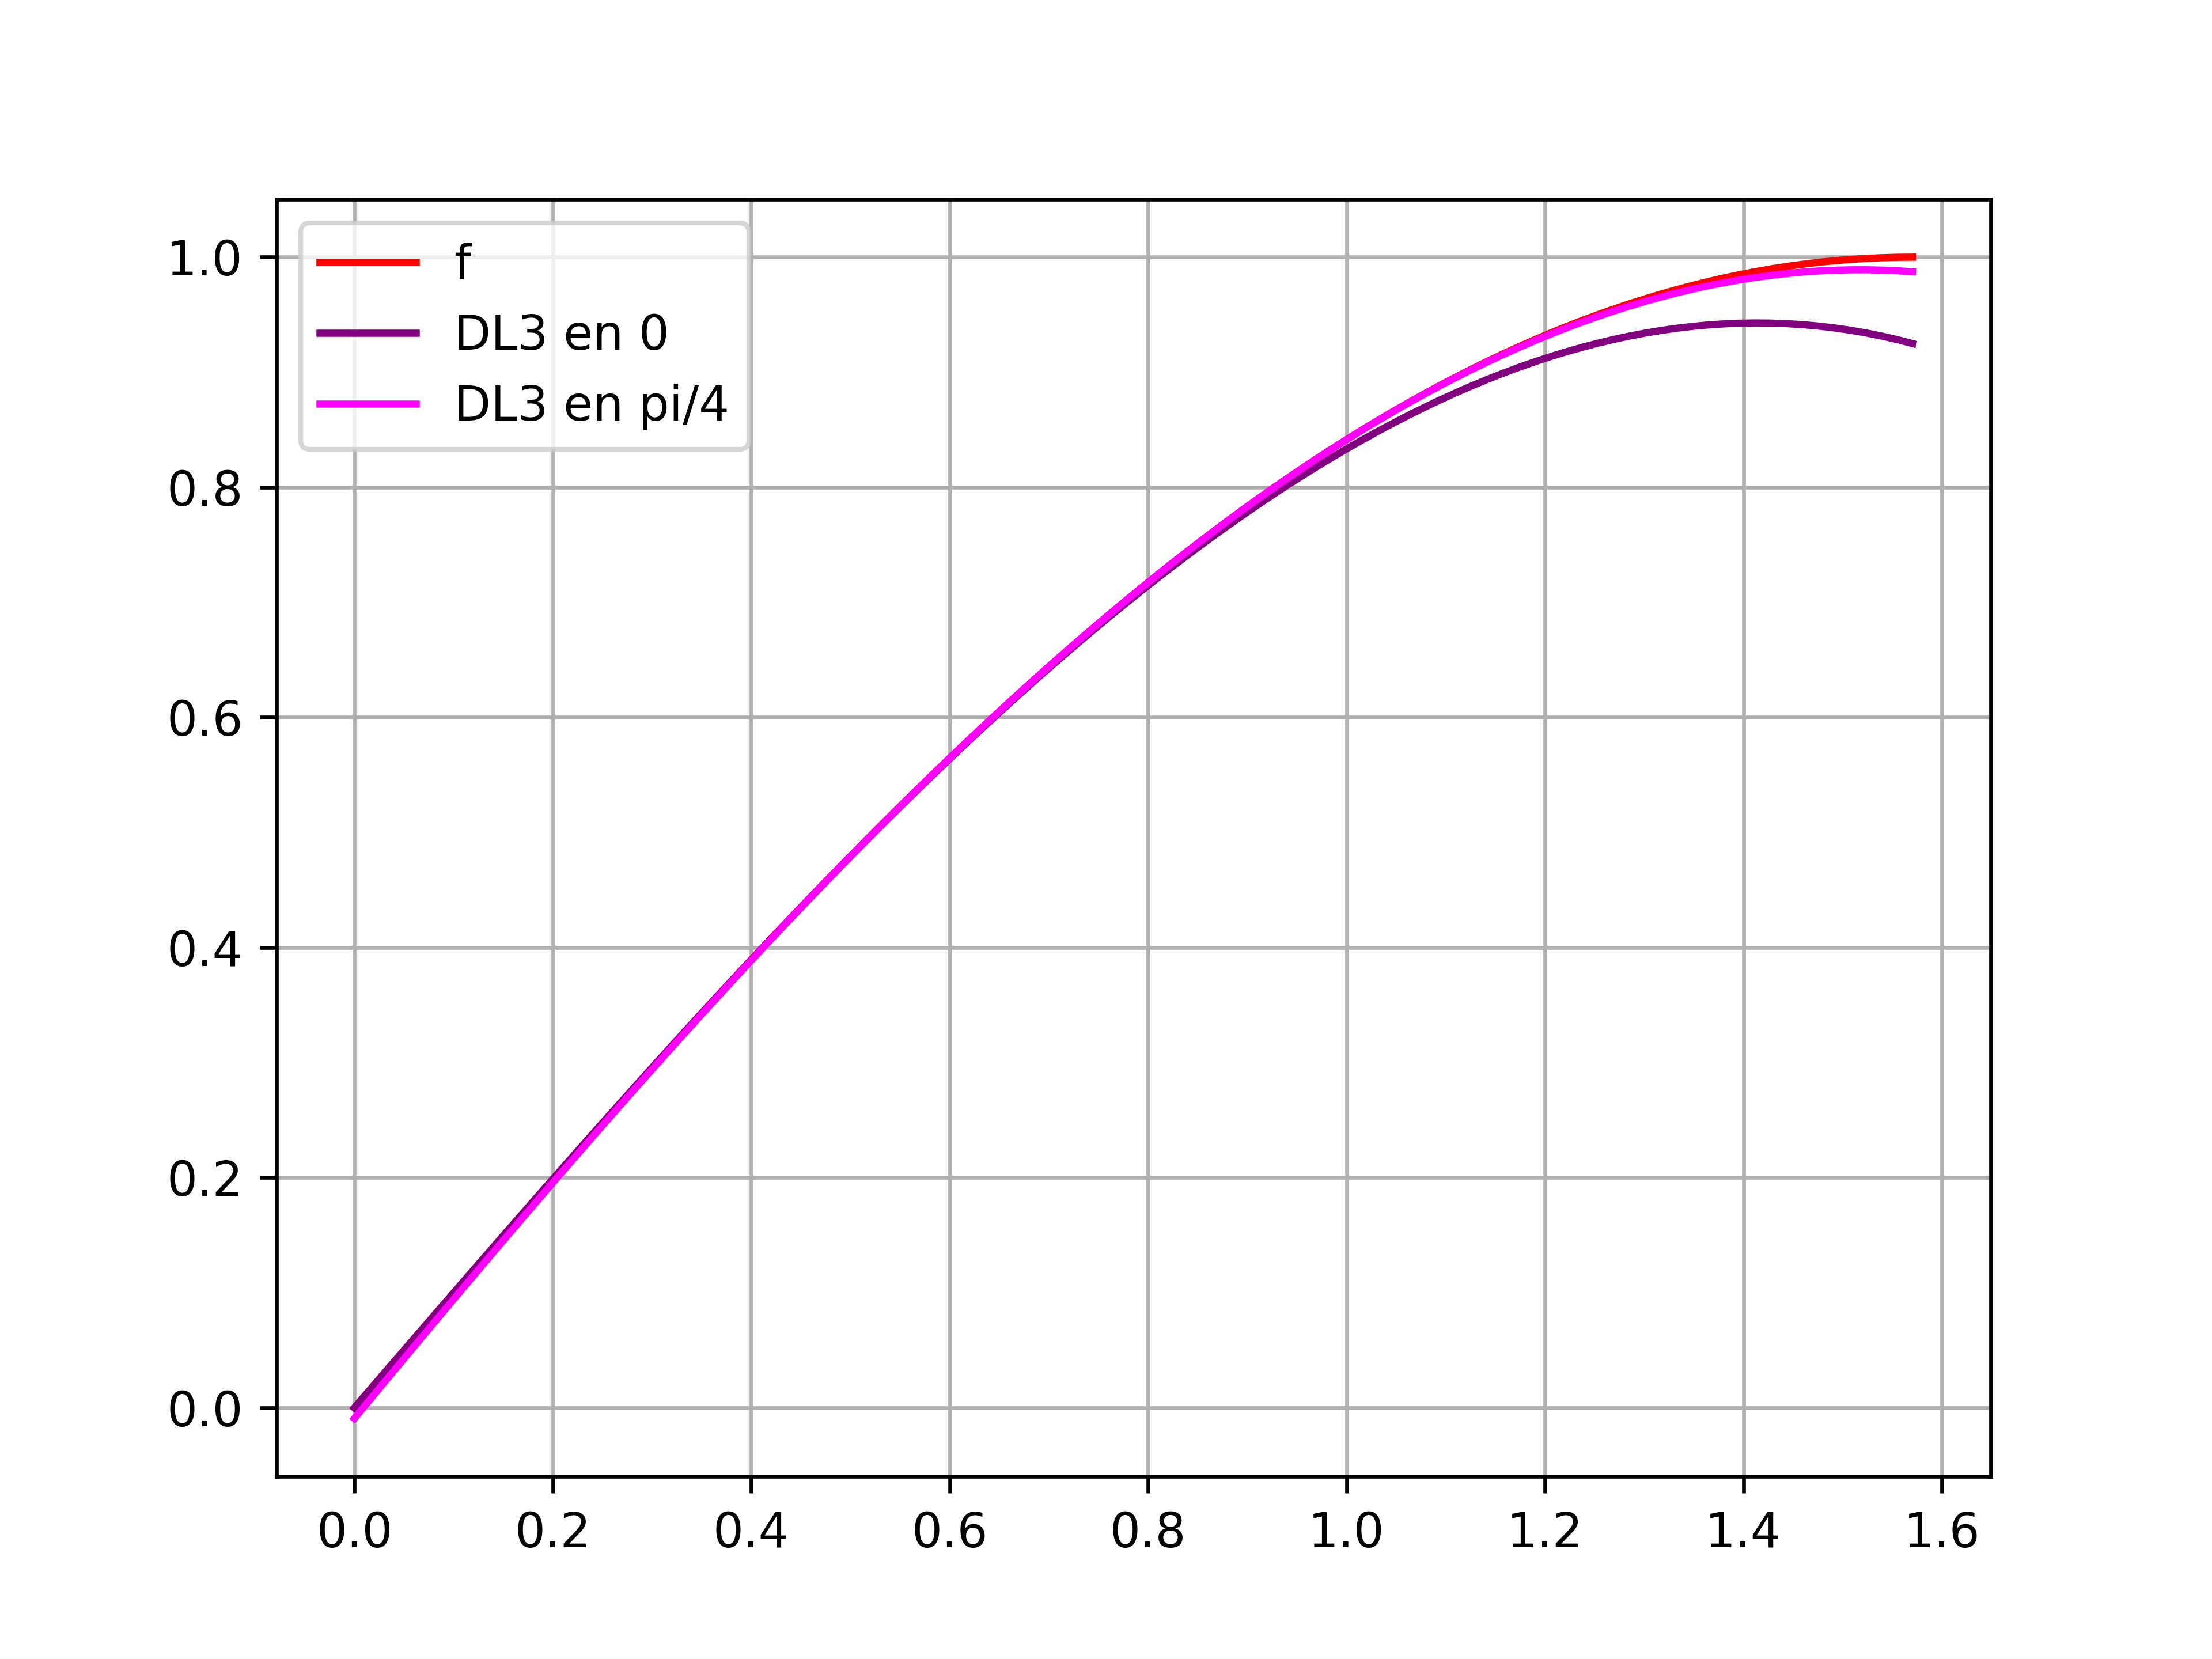
\includegraphics[scale=\myscale,scale=0.5]{figures/approx-dl-03}
  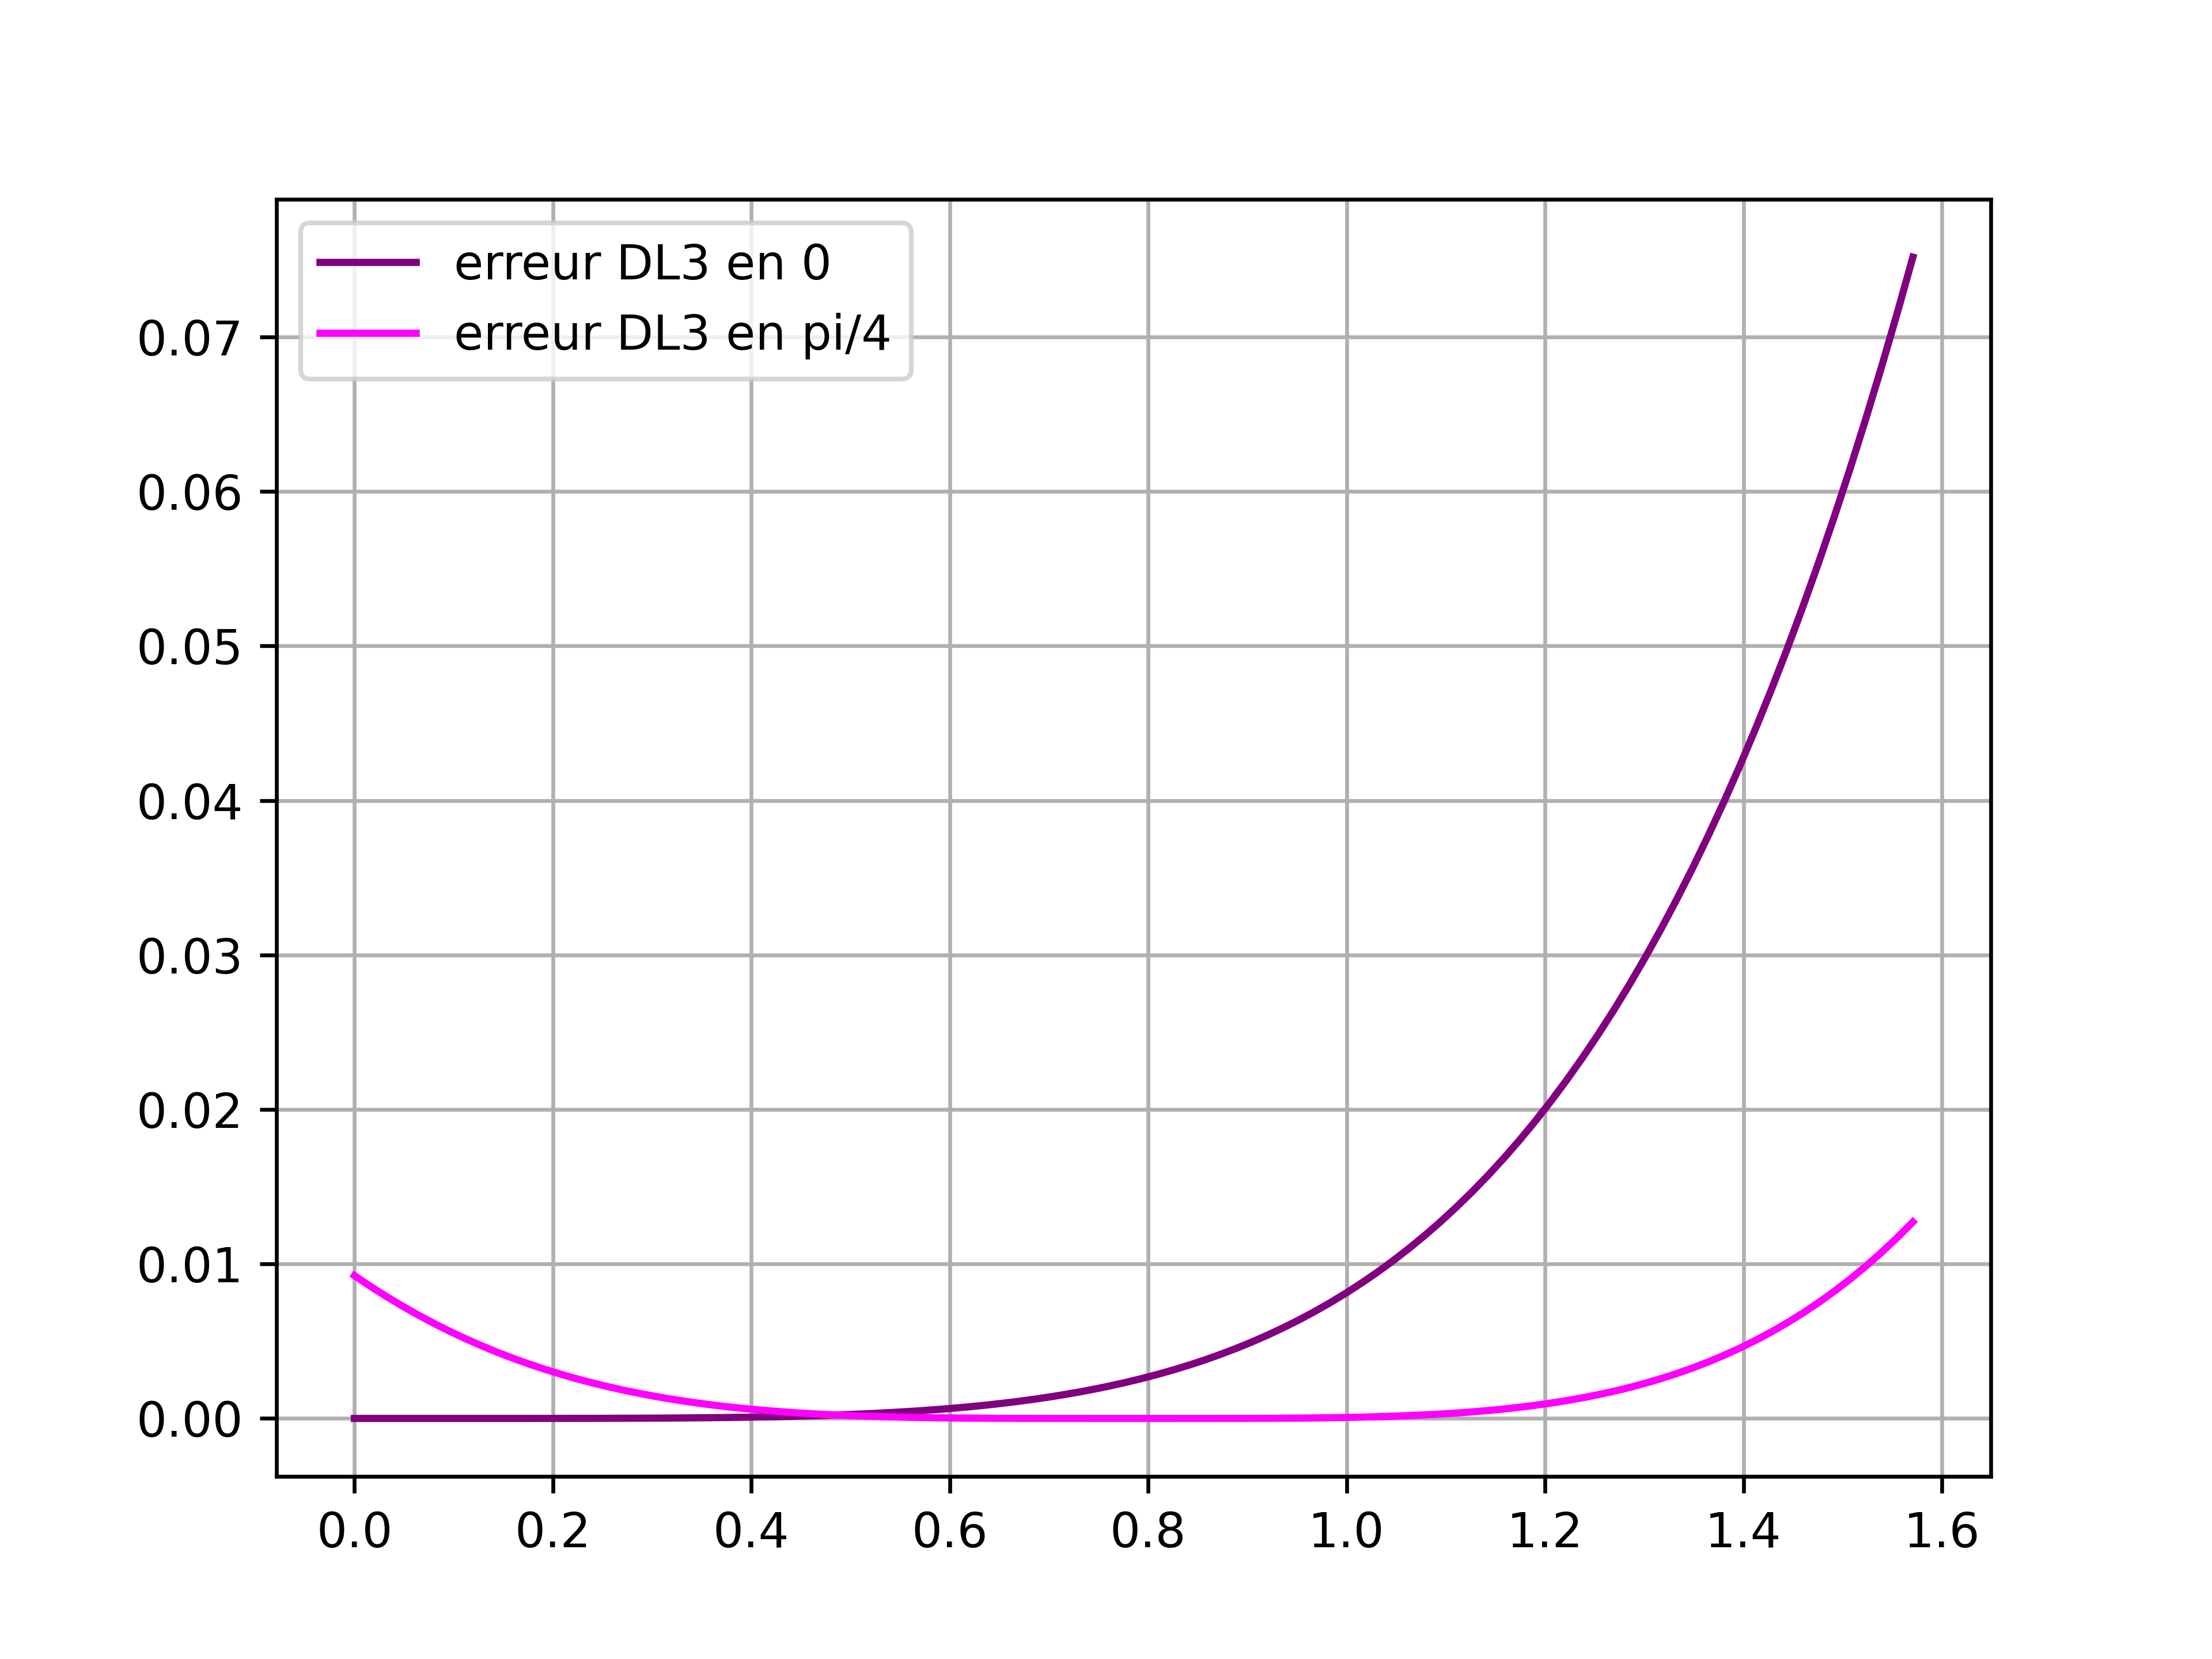
\includegraphics[scale=\myscale,scale=0.5]{figures/approx-dl-04} 
\end{center}

\textbf{Temps de calculs.}
Si on n'a pas besoin d'une grande précision mais d'une grande vitesse de calcul, 
remplacer le calcul de $\sin(x)$ par un DL à l'ordre $3$ est une bonne idée.

\end{exemple}


Voici les premiers termes des développements limités de fonctions usuelles autour de $x_0 = 0$ :
\begin{align*}
\exp(x) &\simeq 1+x+\frac{x^2}{2!}+\frac{x^3}{3!} + \frac{x^4}{4!} + \cdots \\
\sqrt{1+x} &\simeq 1+\frac{x}{2}-\frac{x^2}{8}+\frac{x^3}{16} + \cdots \\
\sin(x) &\simeq x - \frac{x^3}{3!} + \frac{x^5}{5!} - \frac{x^7}{7!} + \cdots \\
\cos(x) &\simeq 1 - \frac{x^2}{2!} + \frac{x^4}{4!} - \frac{x^6}{6!} + \cdots \\
\tan(x) &\simeq x + \frac{x^3}{3} + \frac{2x^5}{15} + \cdots \\
\ln(1+x) &\simeq x - \frac{x^2}{2} + \frac{x^3}{3} - \frac{x^4}{4} + \cdots \\
\end{align*}


%--------------------------------------------------------------------
\subsection{Deux variables}

Soit $f : \Rr^2 \to \Rr$ une fonction à deux variables. Le DL à l'ordre $1$ de $f$ en $(x_0,y_0)$ est : 
\mybox{$f(x_0+h,y_0+k) \simeq f(x_0,y_0) + h\frac{\partial f}{\partial x}(x_0,y_0) + k\frac{\partial f}{\partial x}(x_0,y_0)$}

Géométriquement le graphe de $f$ (qui est ici une surface) est approché par le plan tangent à ce graphe en $(x_0,y_0)$.


\begin{exemple}
La luminosité perçue dépend de l'intensité $I_0$ de la source et de la distance $R_0$ à cette source selon la formule
$$L = \frac{I_0}{R_0^2}$$
Comment évolue cette luminosité lorsque l'intensité ou la distance change ?
Le DL à l'ordre $1$ de $f(x,y) = \frac{x}{y^2}$ en $(x_0,y_0)$ est :
$$f(x_0+h,y_0+k) \simeq  \frac{x_0}{y_0^2} + h\frac{1}{y_0^2} - 2k\frac{x_0}{y_0^3}$$
Ce qui pour notre problème donne :
$$L(I_0 + \Delta I, R_0 + \Delta R) \simeq  \frac{I_0}{R_0^2} + \Delta I\frac{1}{R_0^2} - 2\Delta R\frac{I_0}{R_0^3}$$

Application numérique avec $(I_0,R_0) = (100,10)$, qui donne une luminosité initiale $L(I_0,R_0)=1$, et $\Delta I = 10$ et $\Delta R = 1$ :
$$L(110,11) \simeq 1 + 0.1 - 0.2 = 0.9.$$  
\end{exemple}


%%%%%%%%%%%%%%%%%%%%%%%%%%%%%%%%%%%%%%%%%%%%%%%%%%%%%%%%%%%%%%%%%%%%%
\section{Courbes de Bézier}

%--------------------------------------------------------------------
\subsection{Cubique de Bézier}

\index{courbe!cubique de Bezier@cubique de Bézier}

Expliquons intuitivement les contraintes pour tracer une courbe de Bézier dans l'un des cas le plus simple.
On se donne deux points $A$ et $B$, ainsi que deux vecteurs : un vecteur $\vec{v_A}$ issu de $A$ et un vecteur $\vec{v_B}$ issu de $B$.
La cubique de Bézier est une courbe qui passe par $A$ et $B$ et dont les tangentes sont données par les vecteurs $\vec{v_A}$ et $\vec{v_B}$.
Plus les vecteurs sont grands, plus la courbe reste tangente à ces vecteurs.

\myfigure{1}{
	\tikzinput{fig-bezier-01}
}

Comme on contrôle le vecteur tangent aux extrémités, on peut en recoller deux ensembles de façon à obtenir une courbe globale lisse.
\myfigure{0.8}{
	\tikzinput{fig-bezier-02}
}


Revenons à la définition mathématique de la cubique de Bézier.
Soient $P_0,P_1,P_2,P_3 \in \Rr^2$ quatre points du plan. 
On appelle \defi{cubique de Bézier} le graphe de la fonction $\gamma : [0,1] \to \Rr^2$ définie par :
\mybox{$\gamma(t) = (1-t)^3P_0 \ + \  3(1-t)^2tP_1 \  + \  3(1-t)t^2P_2 \  + \  t^3P_3$}

Cette courbe part de $P_0$ suivant le vecteur tangent $\vec{P_0P_1}$ puis arrive à $P_3$ suivant le vecteur tangent $\vec{P_2P_3}$
(ainsi $P_0$ joue le rôle de $A$, $P_3$ celui de $B$ et $\vec{v_A} = \vec{P_0P_1}$ et $\vec{v_B} = \vec{P_3P_2}$).
Attention la courbe ne passe pas par les points $P_1$ et $P_2$ !

\myfigure{0.8}{
	\tikzinput{fig-bezier-03}
}


Il faut comprendre l'addition de points comme une addition de vecteurs de $\Rr^2$ : 
$aP+bQ$ a pour coordonnées $(a x_P + b x_Q, a y_P + b y_Q)$.
Ainsi pour $t = 0$ on a $\gamma(0) = P_0$ et pour $t = 1$ on a $\gamma(1) = P_3$.

Voici différents exemples de courbes de Bézier.
Tout d'abord si on change la position du point d'arrivée $P_3$ seulement.

\myfigure{0.8}{
	\tikzinput{fig-bezier-04}
}

Ci-dessous on change seulement les vecteurs tangents.

\myfigure{0.7}{
	\tikzinput{fig-bezier-05}
}

La courbe de Bézier peut parfois avoir des formes surprenantes, par exemple elle peut se recouper elle-même.

\myfigure{0.8}{
	\tikzinput{fig-bezier-06}
}


\emph{Bounding box.} Noter que la courbe de Bézier est toujours contenue dans le quadrilatère convexe de sommets $P_0,P_1,P_2,P_3$.
Cela permet d'obtenir un rectangle appelé \emph{bounding box} (ou boîte englobante) de cette courbe. Attention, ce rectangle 
n'est pas nécessairement le rectangle minimal pour la courbe de Bézier.

\myfigure{0.8}{
	\tikzinput{fig-bezier-07}
}

%--------------------------------------------------------------------
\subsection{Vecteur tangent}

\index{vecteur!tangent}

Soit $\gamma : [0,1] \to \Rr^2$ une courbe de Bézier cubique donnée par :
$$\gamma(t) = (1-t)^3P_0 + 3(1-t)^2tP_1 + 3(1-t)t^2P_2 + t^3P_3$$

Alors le vecteur tangent à la courbe au point $\gamma(t)$ est donné par :
\mybox{$\gamma'(t) = 3(1-t)^2 \vec{P_0P_1} \  + \  6(1-t)t \vec{P_1P_2} \  + \  3t^2 \vec{P_2P_3}$}

Voici la preuve :
\begin{align*}
\gamma'(t) 
  &= \frac{d}{dt} \left( (1-t)^3P_0 + 3(1-t)^2tP_1 + 3(1-t)t^2P_2 + t^3P_3 \right) \\
  &= -3(1-t)^2P_0 -6(1-t)t P_1 + 3(1-t)^2 P_1  + 6(1-t)t P_2 - 3t^2 P_2 + 3t^2P_3 \\
  &= 3(1-t)^2 (P_1-P_0) + 6(1-t)t (P_2-P_1) + 3t^2 (P_3-P_2) \\
  &= 3(1-t)^2 \vec{P_0P_1} + 6(1-t)t \vec{P_1P_2} + 3t^2 \vec{P_2P_3}
\end{align*}

Ainsi le vecteur tangent initial (au point $\gamma(0) = P_0$) est :
$$\gamma'(0) = 3 \vec{P_0P_1}.$$
Celui à la fin (au point $\gamma(1) = P_3$) est :
$$\gamma'(1) = -3 \vec{P_3P_2}.$$
Ainsi la courbe est bien tangente au départ et à l'arrivée aux vecteurs $\vec{P_0P_1}$ et $\vec{P_3P_2}$.

\myfigure{0.7}{
	\tikzinput{fig-bezier-08}
}


Une fois que l'on connaît le vecteur tangent $\vec v = (a,b)$ en un point de la courbe, on calcule simplement le vecteur 
normal $\vec n = (-b,a)$, qui est un vecteur perpendiculaire à la tangente à la courbe.

\myfigure{0.6}{
	\tikzinput{fig-bezier-11}
}
Il est utile de rendre ces vecteurs normaux unitaires.

\myfigure{0.9}{
	\tikzinput{fig-bezier-09}
}
Connaître les vecteurs tangents et normaux unitaires permet de dessiner le long d'une courbe, 
tracer une courbe parallèle (comme des rails, mais attention le second rail n'est pas un translaté du premier) ou bien de dessiner ou d'écrire du texte le long d'une courbe.

\begin{center}
  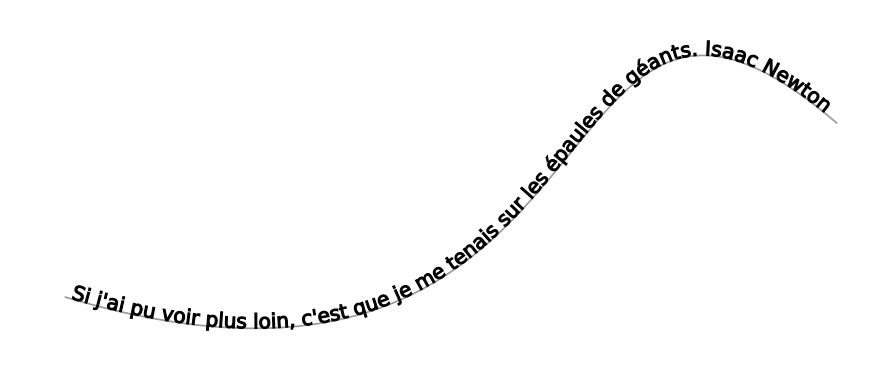
\includegraphics[scale=\myscale,scale=0.4]{figures/texte-bezier}
\end{center}



%--------------------------------------------------------------------
\subsection{Construction récursive}

Pierre Bézier (1910-1999) était ingénieur chez Renault et cherchait des courbes simples à calculer et à dessiner.
C'est Paul de Casteljau (1930-2022, ingénieur chez Citroën !) qui propose un algorithme pour construire facilement les courbes de Bézier.

\textbf{Avec deux points.}
Soient $P_0,P_1 \in \Rr^2$ deux points du plan.
La courbe de Bézier est alors simplement le segment $[P_0,P_1]$ paramétré par :
$$\gamma(t) = (1-t)P_0 + tP_1$$

\myfigure{1}{
	\tikzinput{fig-bezier-21}
}


Nous parlerons de \defi{paramétrisation linéaire} (abrégé en \emph{lerp} pour \emph{linear interpolation}).
Cela signifie que $\gamma(0) = P_0$ et $\gamma(1) = P_1$ et $\gamma(t)$ est à une distance $t$ de $P_0$ et à une distance $1-t$ de $P_1$ 
(si on suppose que la distance $P_0P_1$ vaut $1$).

\textbf{Avec trois points.}
Soient $P_0,P_1,P_2 \in \Rr^2$ trois points du plan.
Pour tracer la courbe de Bézier, on calcule d'une part la paramétrisation linéaire $Q_0(t)$ du segment $[P_0,P_1]$ 
et d'autre part la paramétrisation linéaire $Q_1(t)$ du segment $[P_1,P_2]$.
Pour chaque $t$, on obtient un segment $[Q_0(t),Q_1(t)]$. On calcule alors la paramétrisation linéaire $R(t)$ de ce segment.
Ce point $R(t)$ est le point de la courbe de Bézier au paramètre $t$.

\myfigure{0.9}{
	\tikzinput{fig-bezier-22}
}
 

\textbf{Avec quatre points.}
On part de quatre points $P_0,P_1,P_2,P_3$, on calcule trois paramétrisations linéaires correspondant aux trois segments, on obtient ainsi
trois points $Q_0(t), Q_1(t), Q_2(t)$, puis on calcule deux paramétrisations linéaires $R_0(t), R_1(t)$ 
correspondant aux deux segments $[Q_0(t), Q_1(t)]$, $[Q_1(t), Q_2(t)]$, 
finalement le point final $S(t)$ de la courbe de Bézier est celui de la paramétrisation linéaire de $[R_0(t), R_1(t)]$.

Noter que cet algorithme est récursif : on calcule le point d'une courbe de Bézier de $n$ points en calculant des points de plusieurs courbes de Bézier de $n-1$ points.
Il faut bien noter que le paramètre $t \in [0, 1]$ est le même pour toutes les courbes de Bézier intermédiaires.

\myfigure{0.8}{
	\tikzinput{fig-bezier-23}
}

%--------------------------------------------------------------------
\subsection{Cas général}

Les formules et constructions précédentes se généralisent pour obtenir la courbe de Bézier pour $n+1$ points $P_0,\ldots,P_n$.

Le  \defi{polynôme de Bernstein} de degré $n$ est défini par :
$$b_{i,n}(t) = \binom{n}{i} t^i (1-t)^{n-i}$$
où $\binom{n}{i} = \frac{n!}{i!(n-i)!}$ est le coefficient binomial \og{}$i$ parmi $n$\fg{}.
La \defi{courbe de Bézier}\index{courbe!de Bezier@de Bézier d'ordre $n$} associée à $P_0,\ldots,P_n$ est alors paramétrée par :
\mybox{$\displaystyle \gamma(t) = \sum_{i=0}^n b_{i,n}(t) P_i$}

\begin{center}
  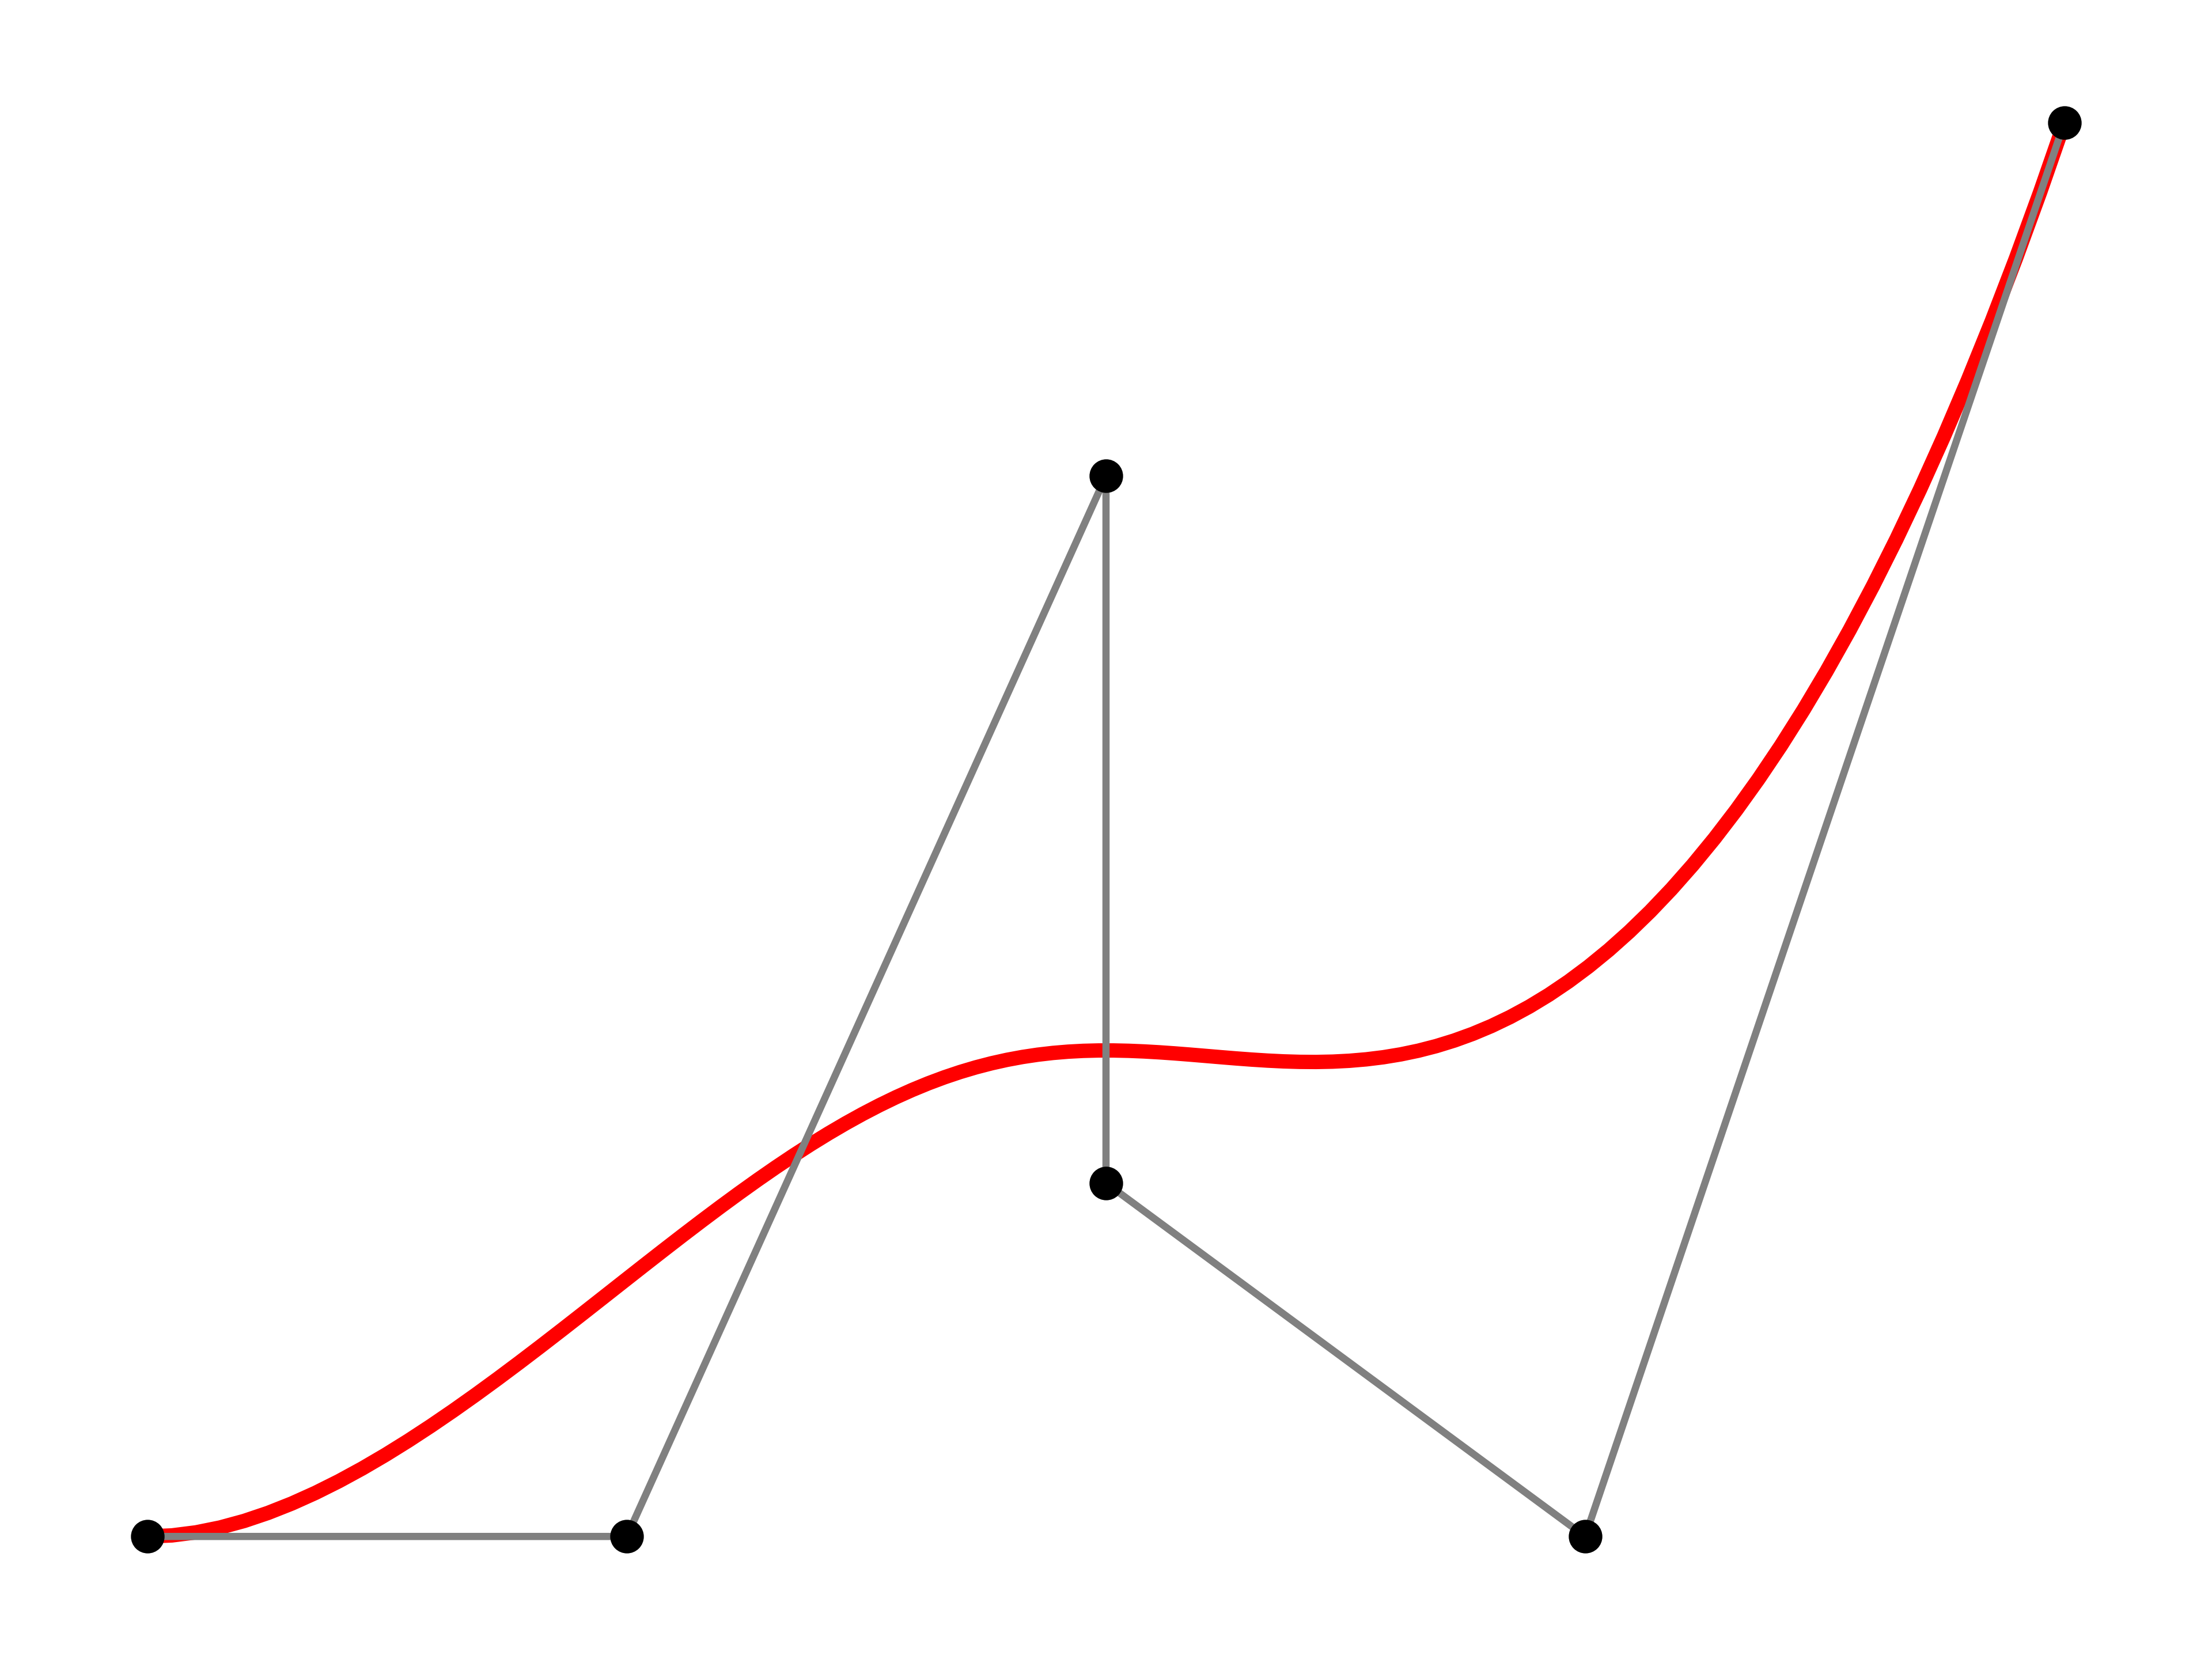
\includegraphics[scale=\myscale,scale=0.4]{figures/approx-bezier-01}
\end{center}



%%%%%%%%%%%%%%%%%%%%%%%%%%%%%%%%%%%%%%%%%%%%%%%%%%%%%%%%%%%%%%%%%%%%%
\section{Approximation globale}

%--------------------------------------------------------------------
\subsection{Interpolation de Lagrange}

\index{interpolation!de Lagrange}

Le problème est le suivant : on nous donne $n+1$ points  dans le plan et on cherche une courbe passant exactement par tous ces points.

Précisons le problème : soient $(a_0,b_0),\ldots,(a_n,b_n)$, $n+1$ points du plan avec $a_0 < a_1 < \cdots < a_n$.
On cherche un polynôme $P(X)$ de degré $\le n$ tel que $P(a_i) = b_i$ pour tout $i=0,\ldots,n$.


\begin{center}
  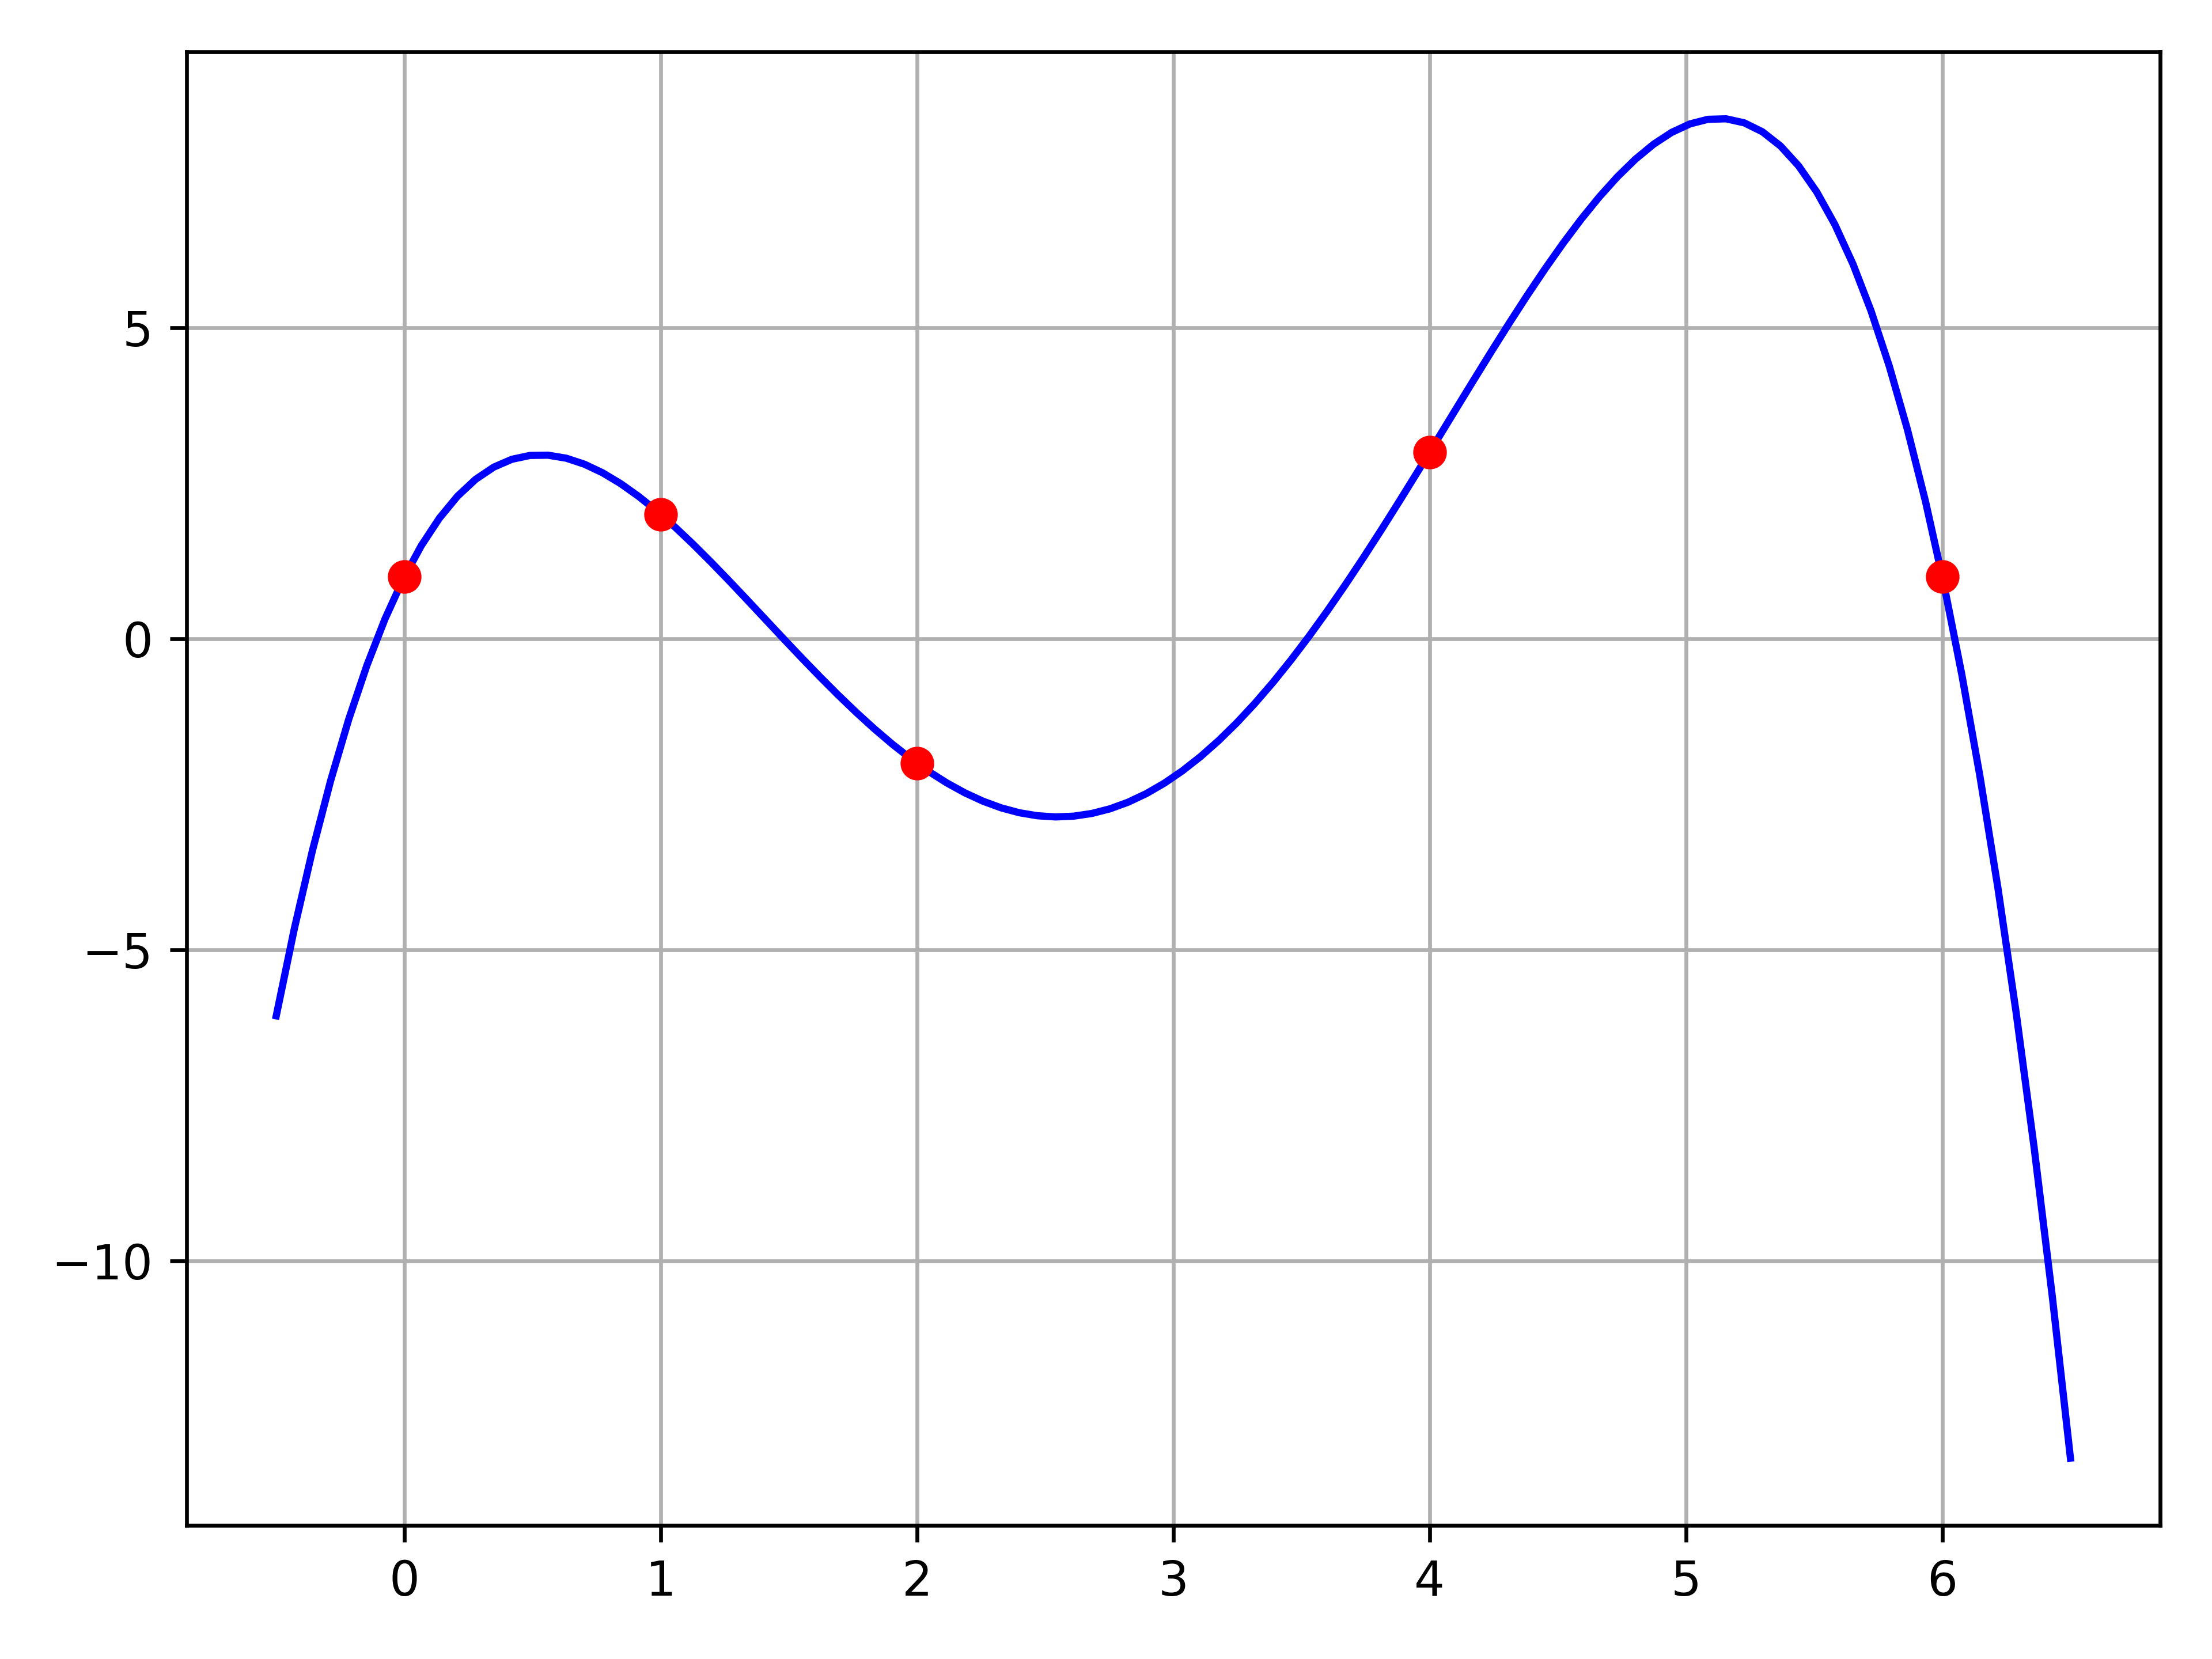
\includegraphics[scale=\myscale,scale=0.5]{figures/approx-lagrange-01}
\end{center}

\begin{proposition}
Si on note le \defi{polynôme de Lagrange élémentaire}
\mybox{$\displaystyle L_i(X) = \prod_{\substack{j=0\\j\neq i}}^n \frac{X-a_j}{a_i-a_j}$}
alors l'unique polynôme de degré $\le n$ vérifiant $P(a_i) = b_i$ pour tout $i=0,\ldots,n$, est :
\mybox{$\displaystyle P(X) = \sum_{i=0}^n b_i L_i(X)$}
\end{proposition}

Pour la preuve le point clé est de remarquer que pour le polynôme élémentaire $L_i(X)$, on a :
$$L_i(a_i) = 1 \qquad \text{ et } \qquad L_i(a_j) = 0 \text{ pour tout } j\neq i.$$ 

\begin{proof}
Montrons d'abord que le polynôme $P(X)$ (qui est bien de degré $n$) convient. En effet 
$$P(a_i) =  \sum_{j=0}^n b_j L_j(a_i) = b_i L_i(a_i) = b_i$$
car pour $j \neq i$, on a $L_j(a_i) = 0$.

Soit maintenant $Q(X)$ un autre polynôme de degré $\le n$ vérifiant $Q(a_i) = b_i$ pour tout $i=0,\ldots,n$.
On a alors ($P-Q)(a_i)=0$ pour tout $i=0,\ldots,n$. Donc le polynôme $P(X)-Q(X)$ est un polynôme de degré $\le n$ ayant 
$n+1$ racines distinctes, c'est donc le polynôme nul. D'où $P(X)=Q(X)$.
\end{proof}

\begin{exemple}
Considérons $n=2$ et les $3$ points $(a_0,b_0)$, $(a_1,b_1)$ et $(a_2,b_2)$.
Trouvons l'équation de l'unique parabole passant par ces trois points. 
Tout d'abord :
$$L_0(X) = \frac{(X-a_1)(X-a_2)}{(a_0-a_1)(a_0-a_2)} \qquad L_1(X) = \frac{(X-a_0)(X-a_2)}{(a_1-a_0)(a_1-a_2)} \qquad L_2(X) = \frac{(X-a_0)(X-a_1)}{(a_2-a_0)(a_2-a_1)}$$
et donc
$$P(X) = b_0 L_0(X) + b_1 L_1(X) + b_2 L_2(X).$$

Par exemple pour les points $(0,2)$, $(1,1)$ et $(3,4)$, on a :
$$L_0(X) = \frac{(X-1)(X-3)}{(0-1)(0-3)} = \frac{1}{3}(X^2-4X+3)$$
$$L_1(X) = \frac{(X-0)(X-3)}{(1-0)(1-3)} = -\frac{1}{2}(X^2-3X)$$
$$L_2(X) = \frac{(X-0)(X-1)}{(3-0)(3-1)} = \frac{1}{6}(X^2-X)$$
et donc
$$P(X) = \frac{2}{3}(X^2-4X+3) \ - \ \frac{1}{2}(X^2-3X) \  + \  \frac{4}{6}(X^2-X)
= \frac16(5X^2-11X+12)$$

\begin{center}
  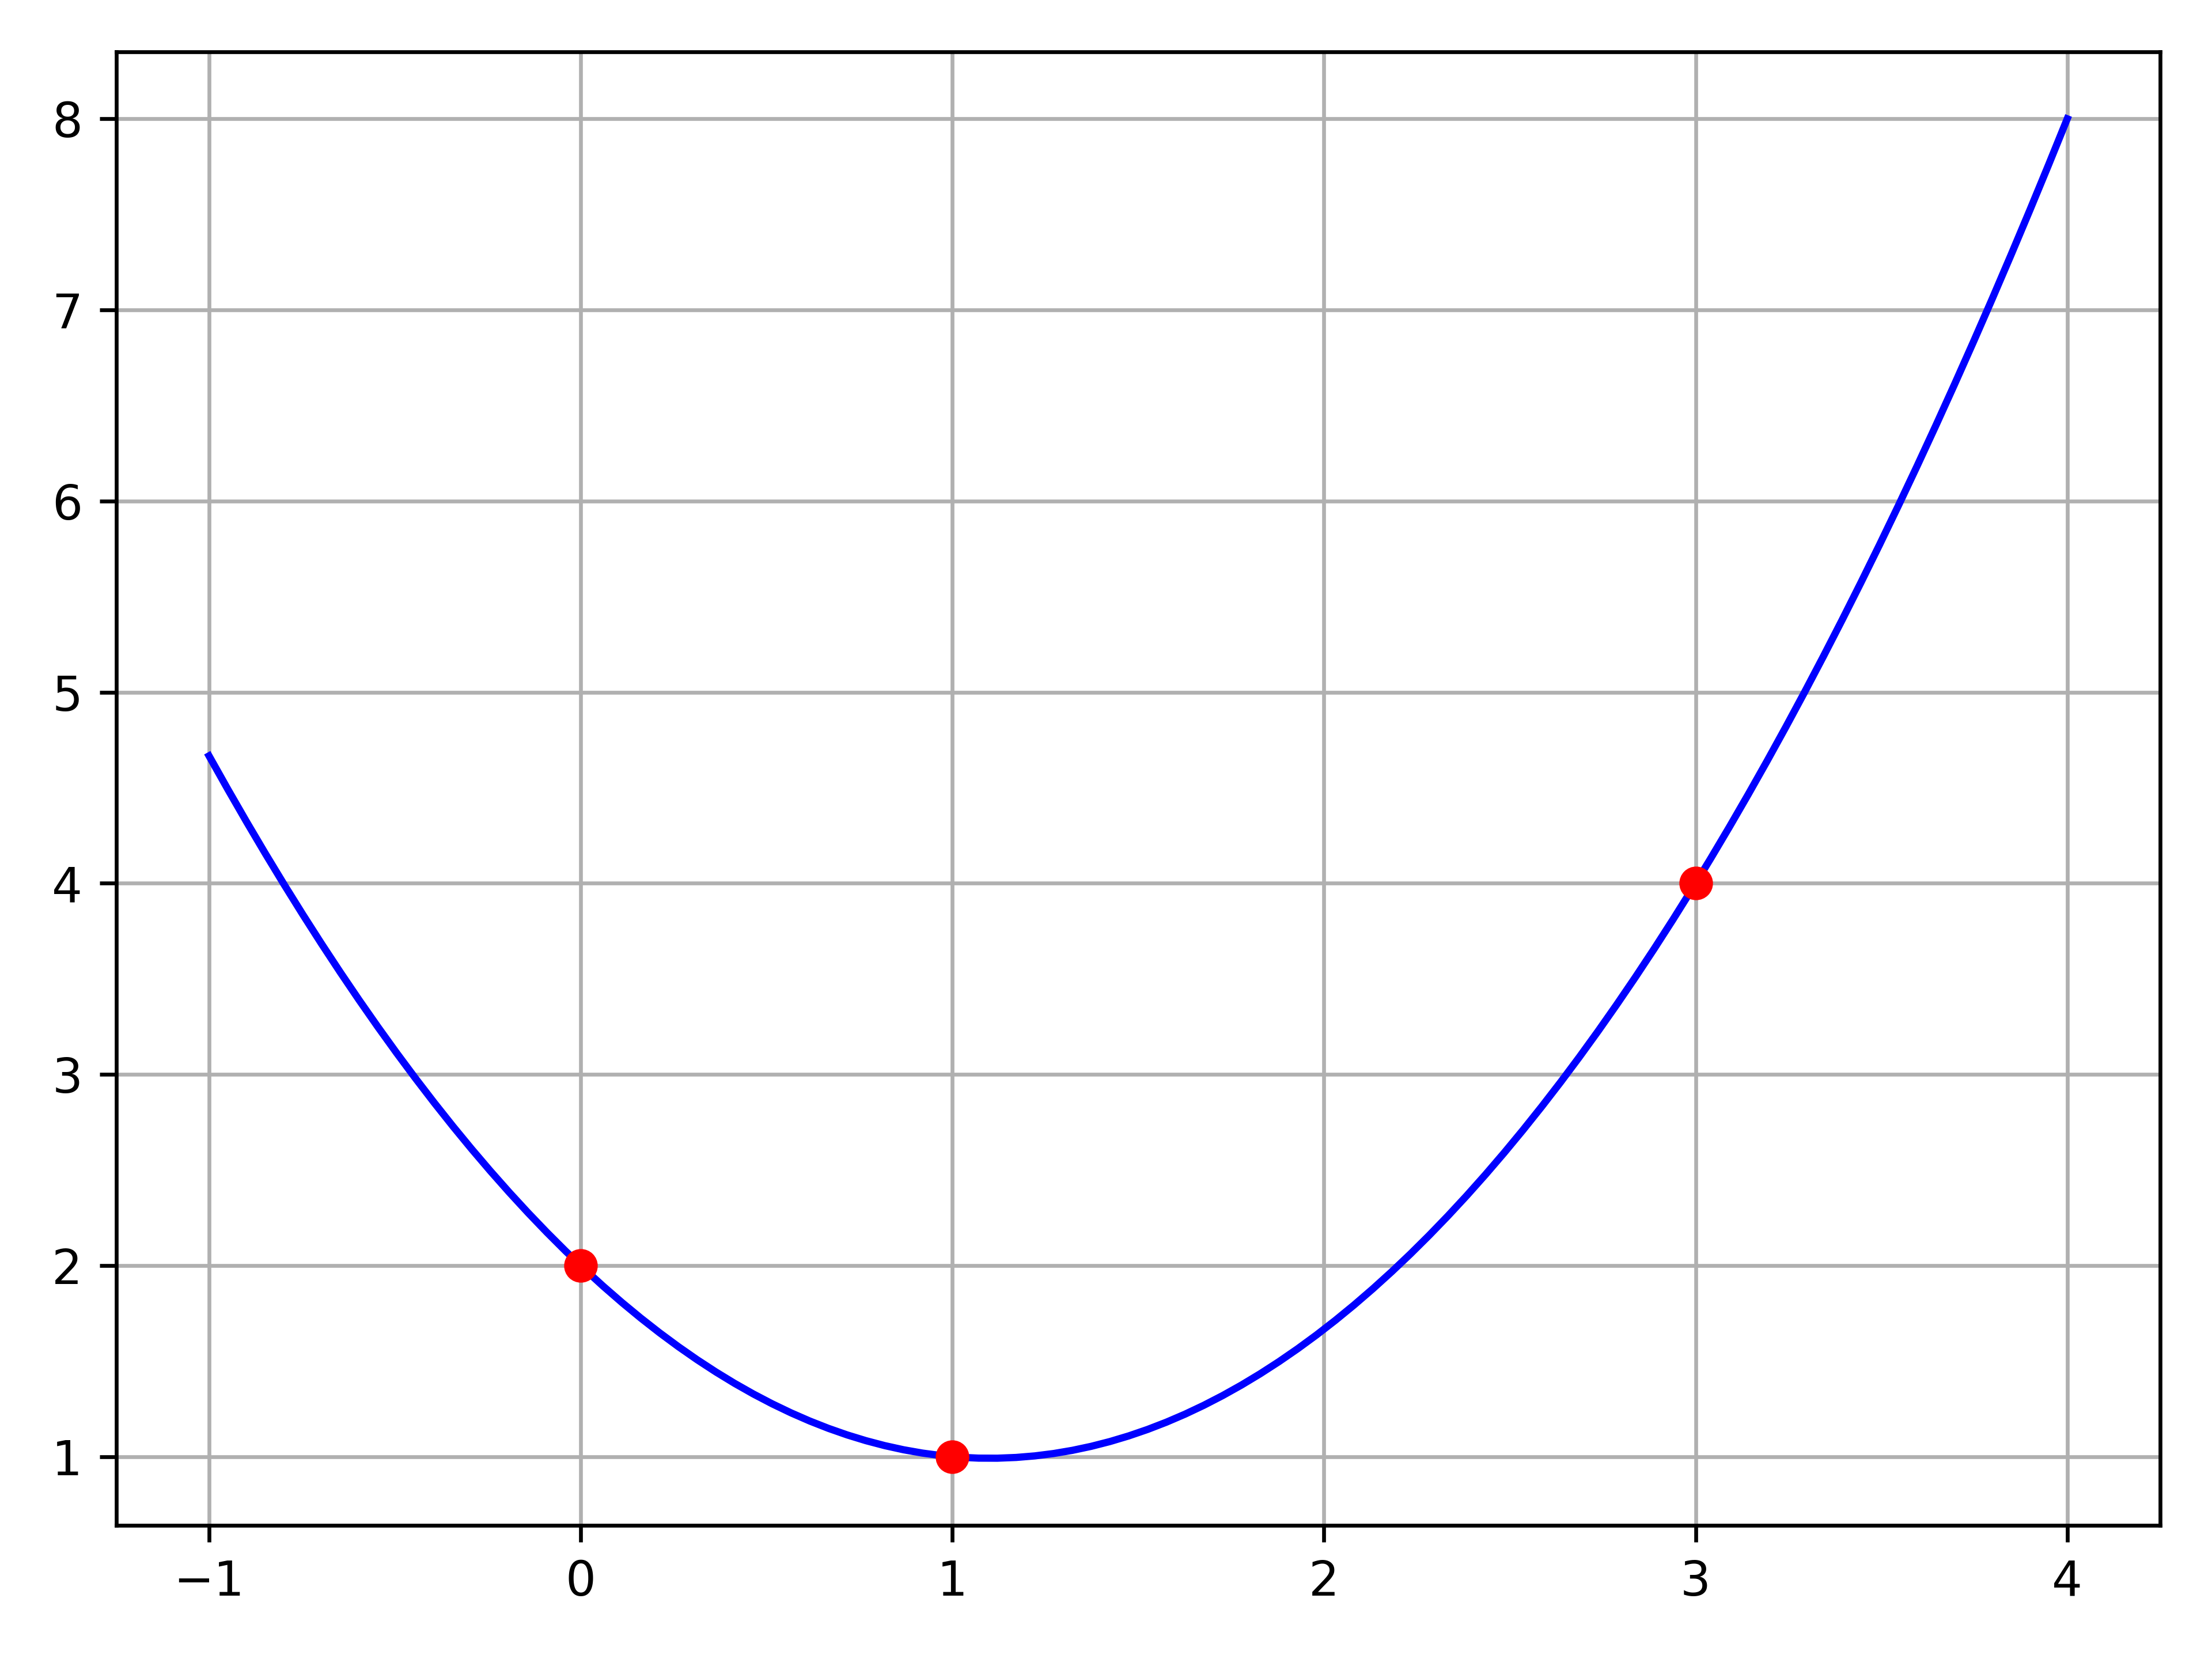
\includegraphics[scale=\myscale,scale=0.5]{figures/approx-lagrange-02}
\end{center}

\end{exemple}

\begin{exemple}
Voici un exemple avec $4$ points ($n=3$).

\begin{center}
  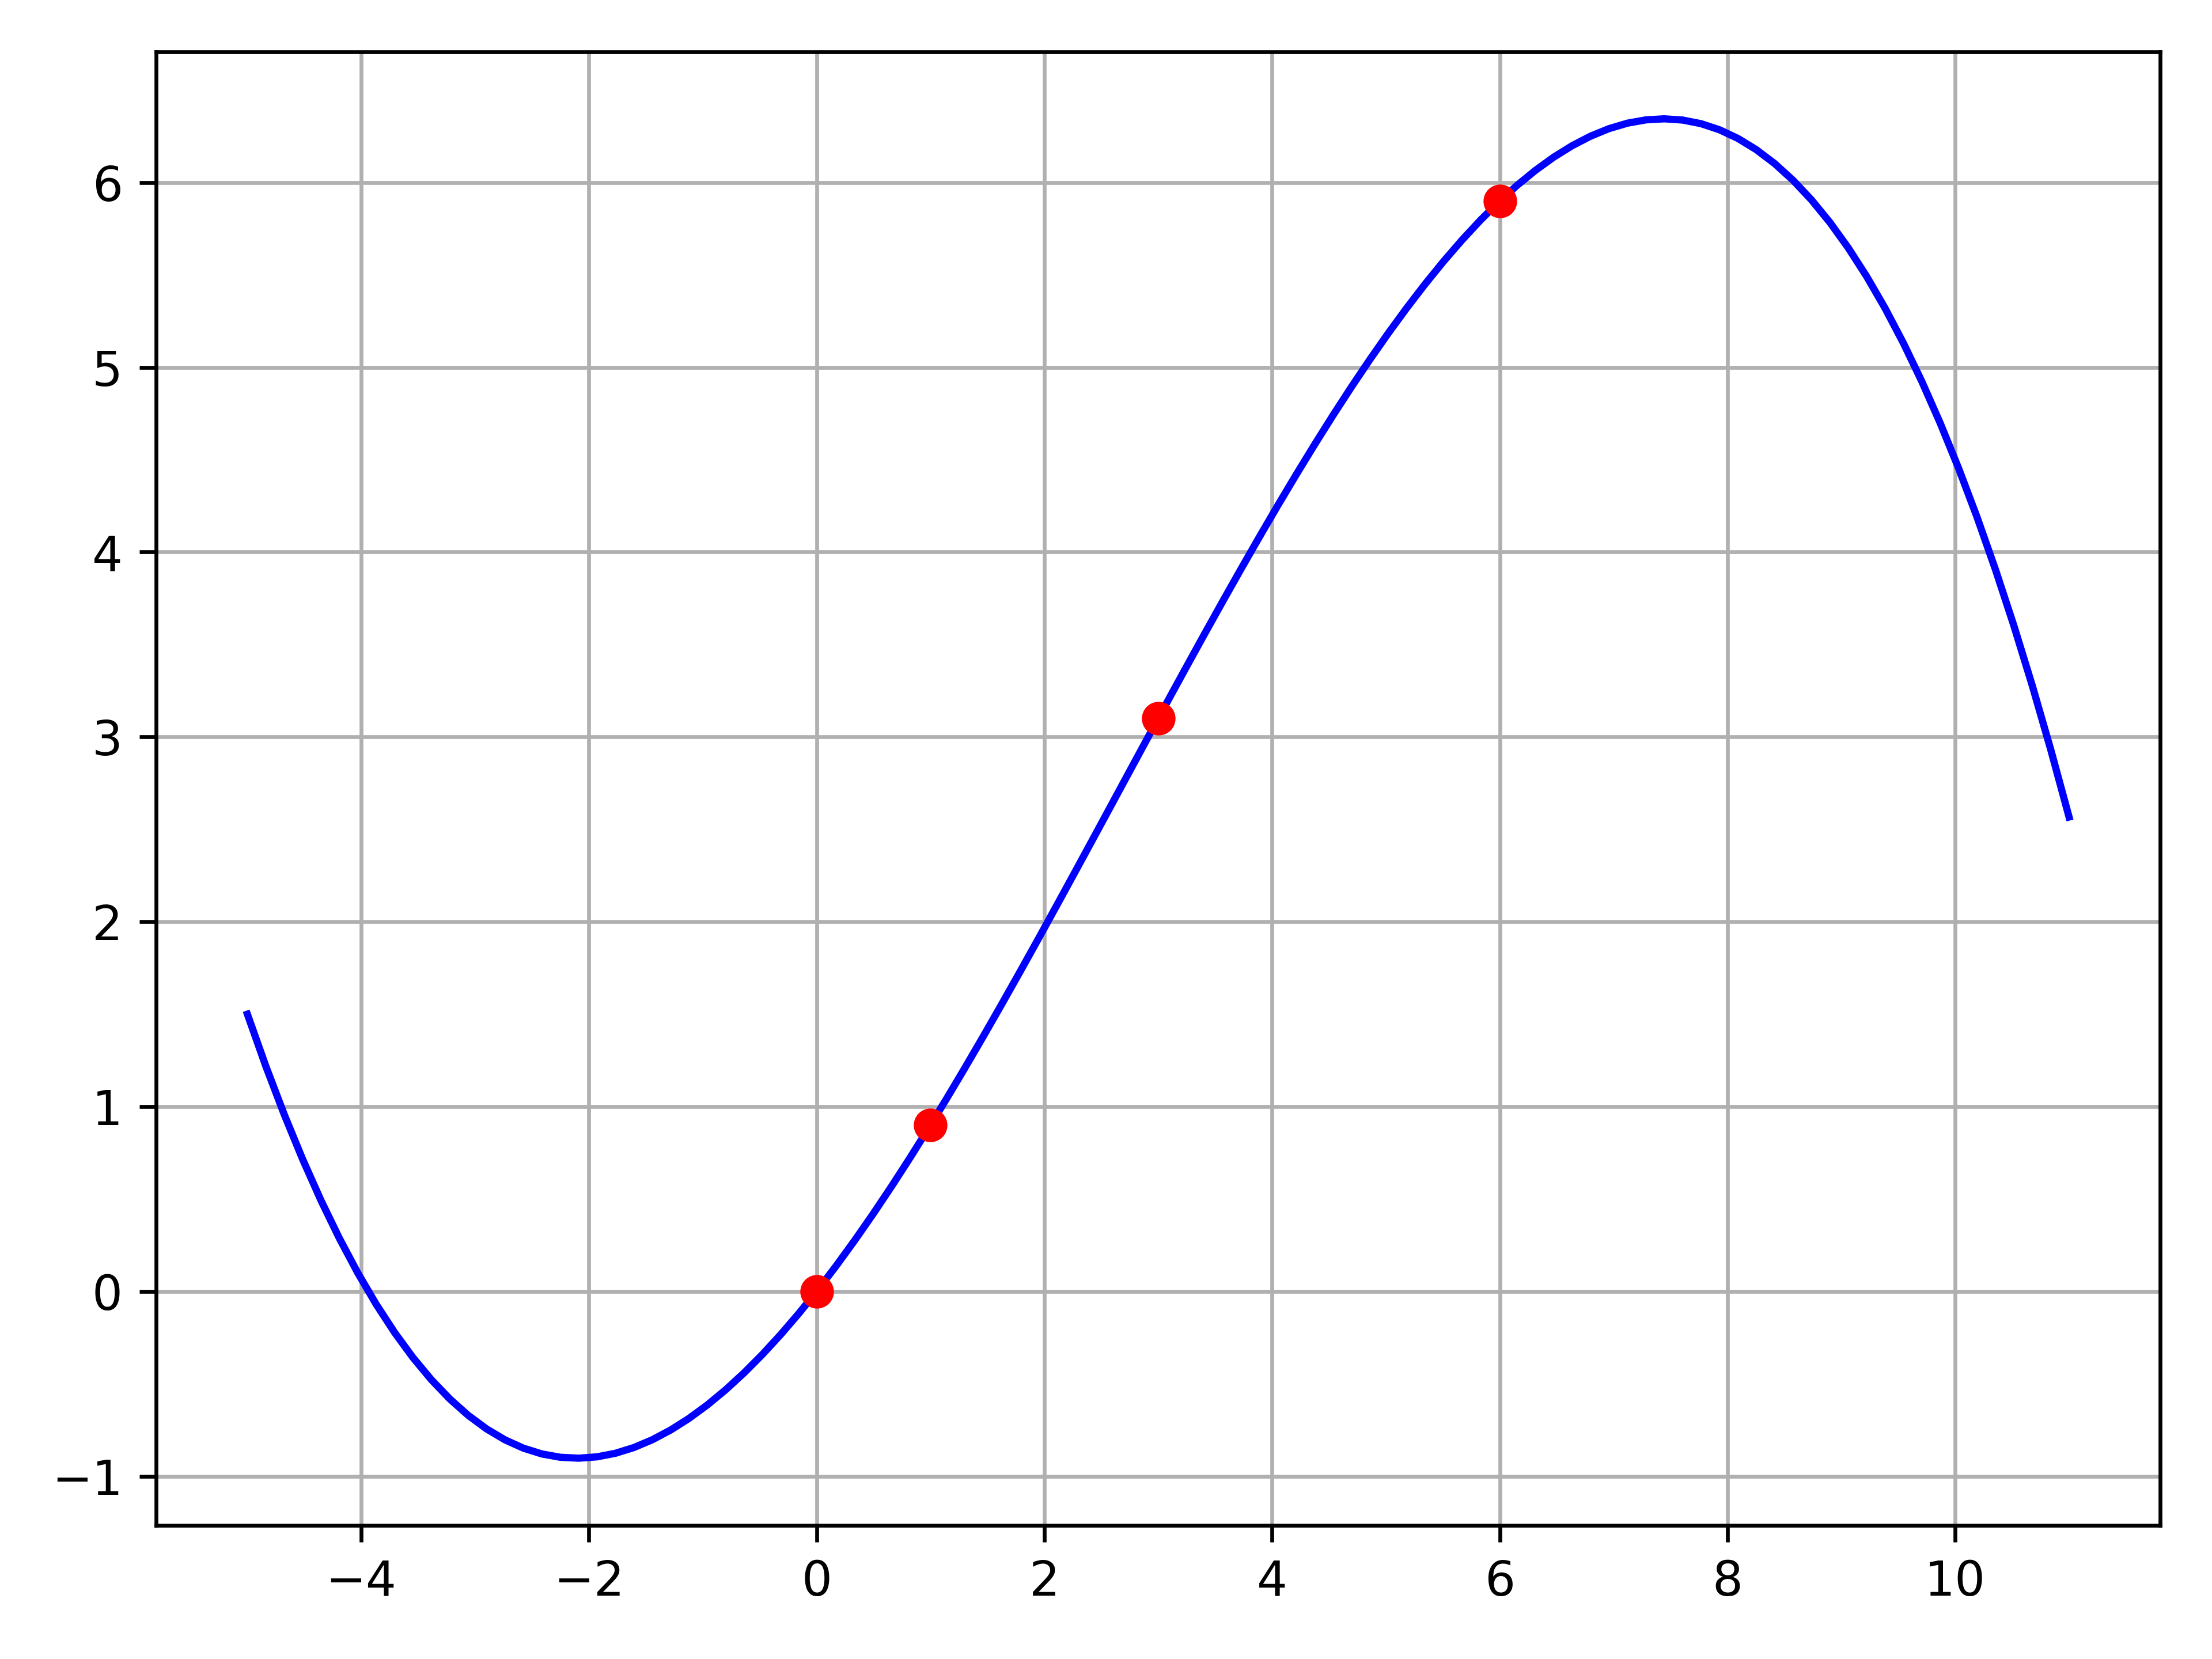
\includegraphics[scale=\myscale,scale=0.5]{figures/approx-lagrange-03}
\end{center}

On remarque que même si ces quatre points sont presque alignés la courbe obtenue est très éloignée d'une courbe affine. 
On peut se demander si imposer de passer exactement par les points n'est pas une contrainte trop forte.
\end{exemple}


%--------------------------------------------------------------------
\subsection{Polynômes de Tchebychev}

\index{approximation!de Tchebychev}

Décrivons deux façons de définir les polynômes de Tchebychev $T_n(X)$.

\textbf{Définition trigonométrique.}
Le polynôme $T_n(X)$ est défini par la relation :
$$T_n(X) = \cos(n \arccos X)$$
Autrement dit :
\mybox{$\displaystyle T_n(\cos \theta) = \cos (n \theta)$}



\textbf{Définition par récurrence.}
Le polynôme $T_n(X)$ est aussi défini par la relation de récurrence :
\mybox{$\displaystyle 
T_0(X) = 1 \qquad T_1(X) = X \qquad 
T_{n+1}(X) = 2X T_n(X) - T_{n-1}(X) \qquad \text{ pour } n \ge 1
$}


Voici la liste des premiers polynômes de Tchebychev :
$$T_0(X) = 1 \qquad T_1(X) = X \qquad T_2(X) = 2X^2-1$$
$$T_3(X) = 4X^3-3X \qquad T_4(X) = 8X^4-8X^2+1 \qquad T_5(X) = 16X^5-20X^3+5X$$

Voici les graphes de ces polynômes $T_n(X)$ pour $n=1,\ldots,6$.
\begin{center}
  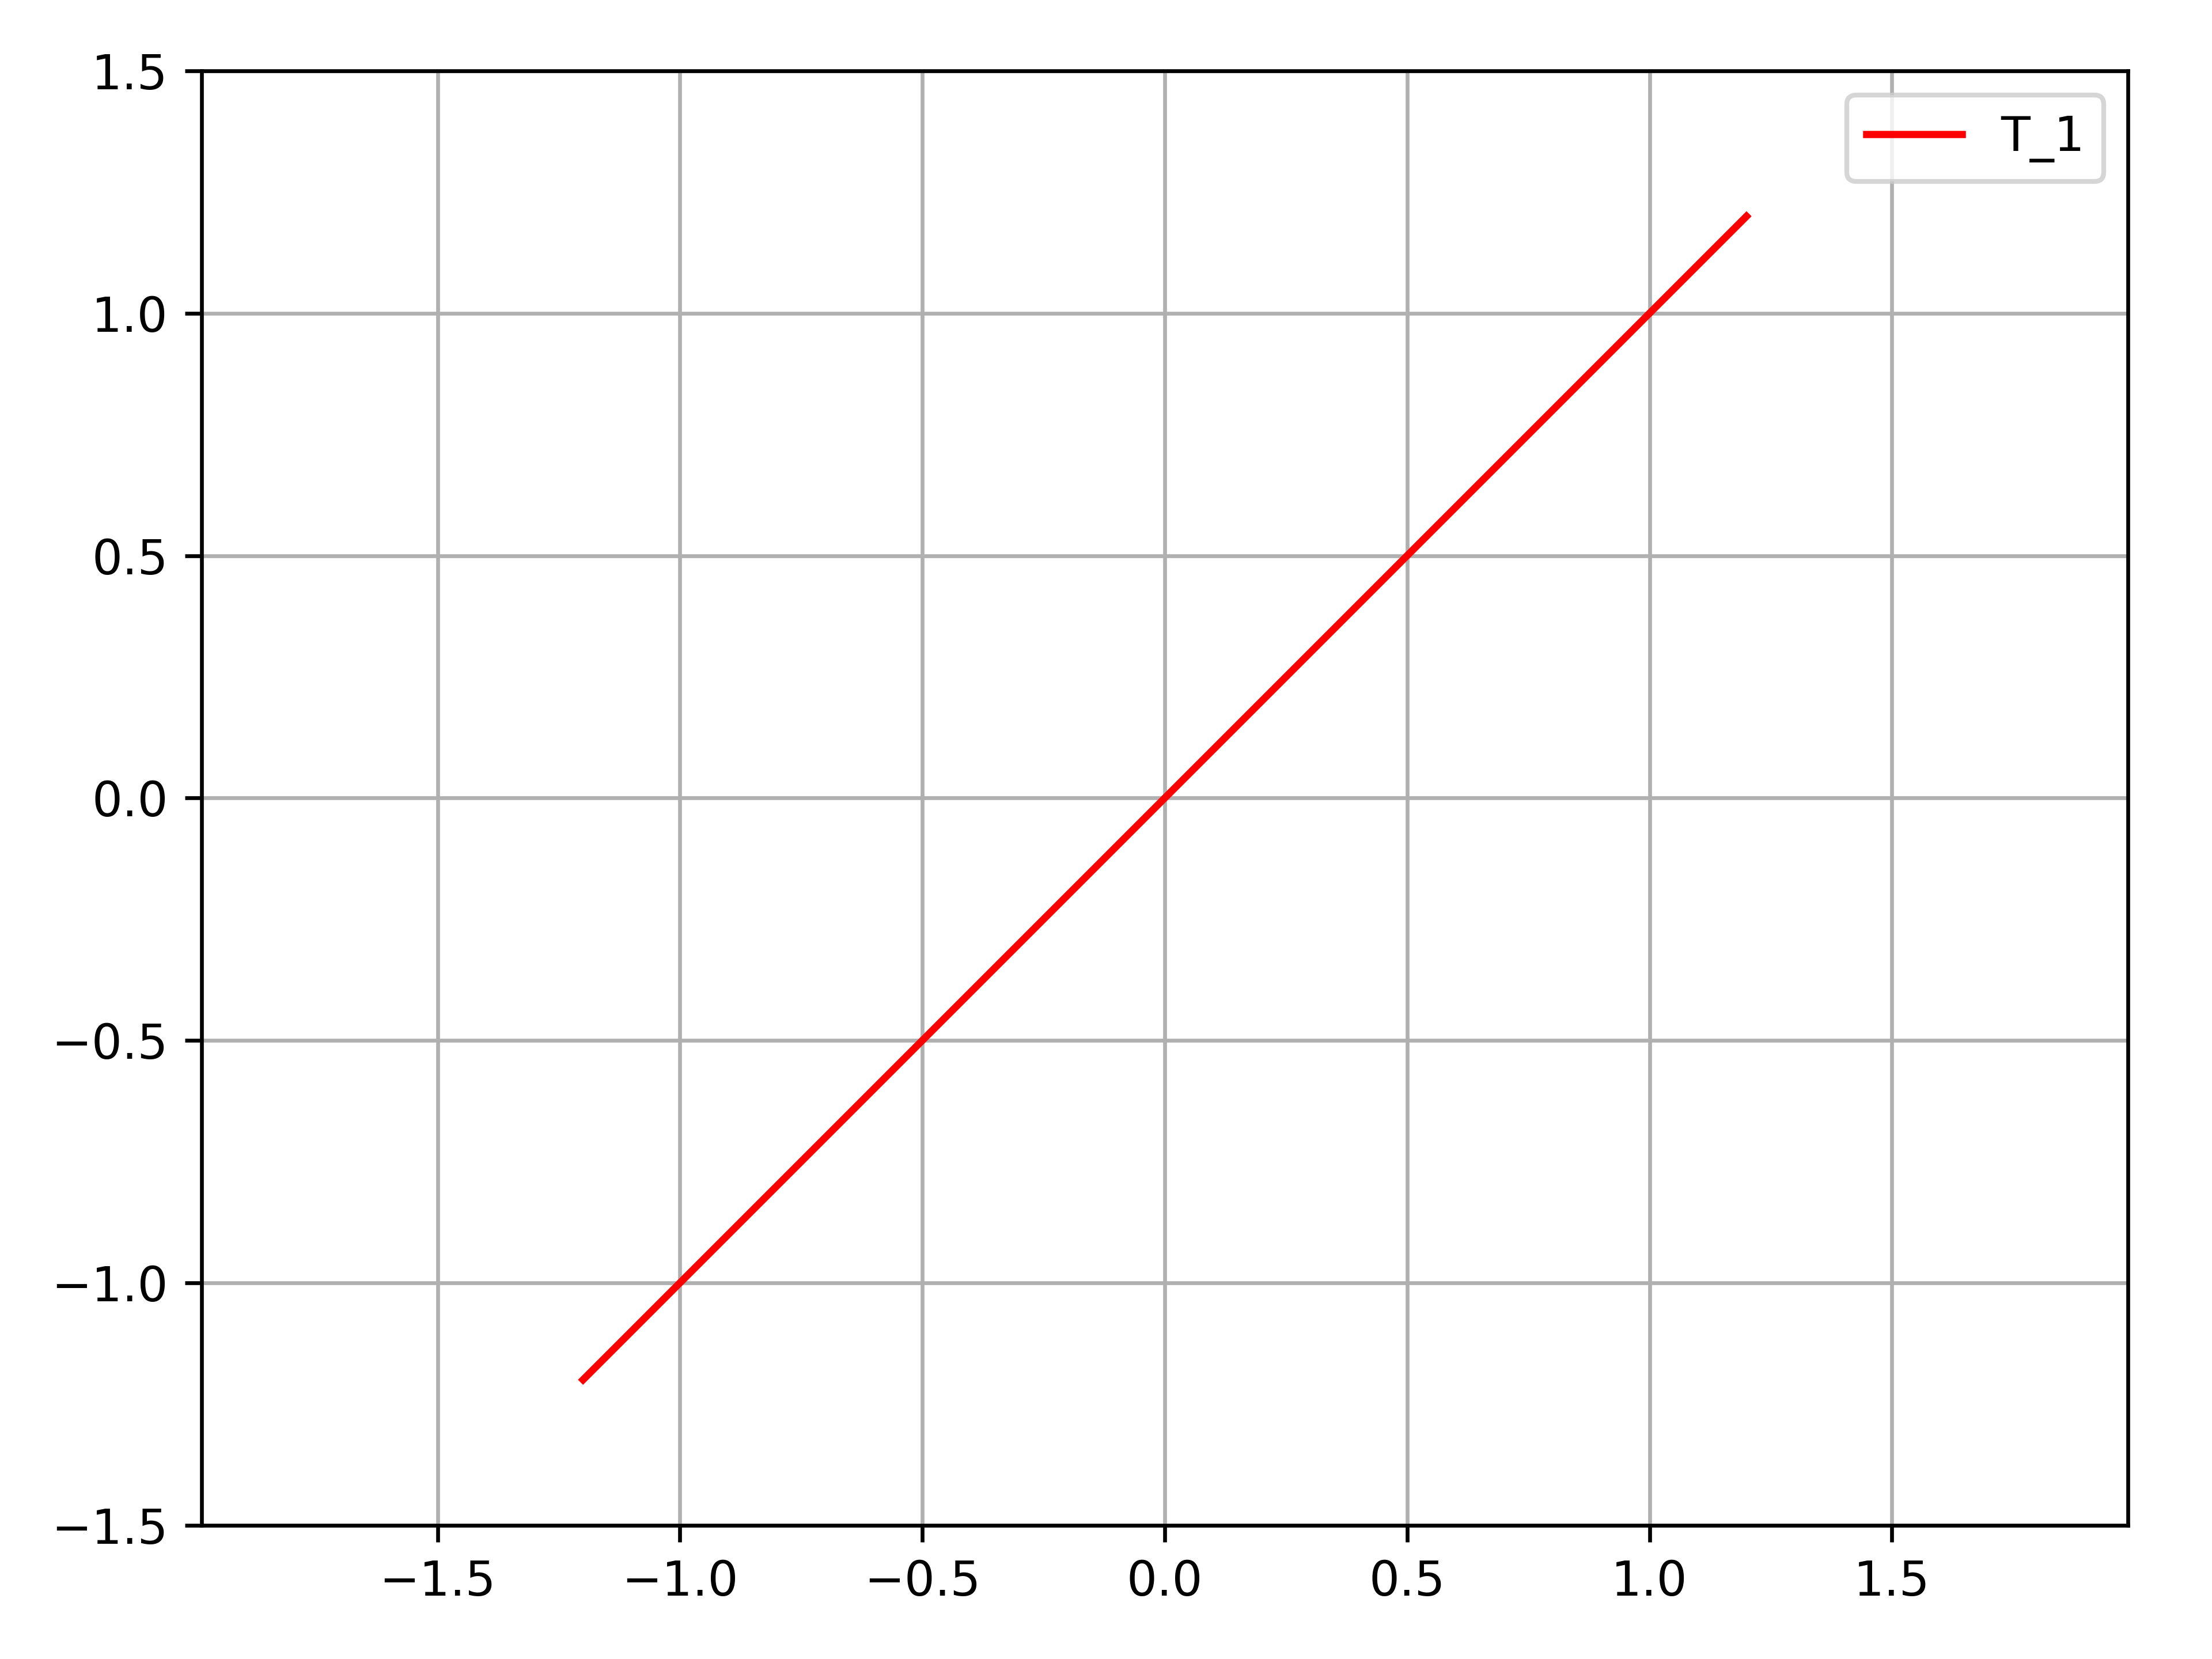
\includegraphics[scale=\myscale,scale=0.3]{figures/approx-tchebychev-01-1} \qquad
  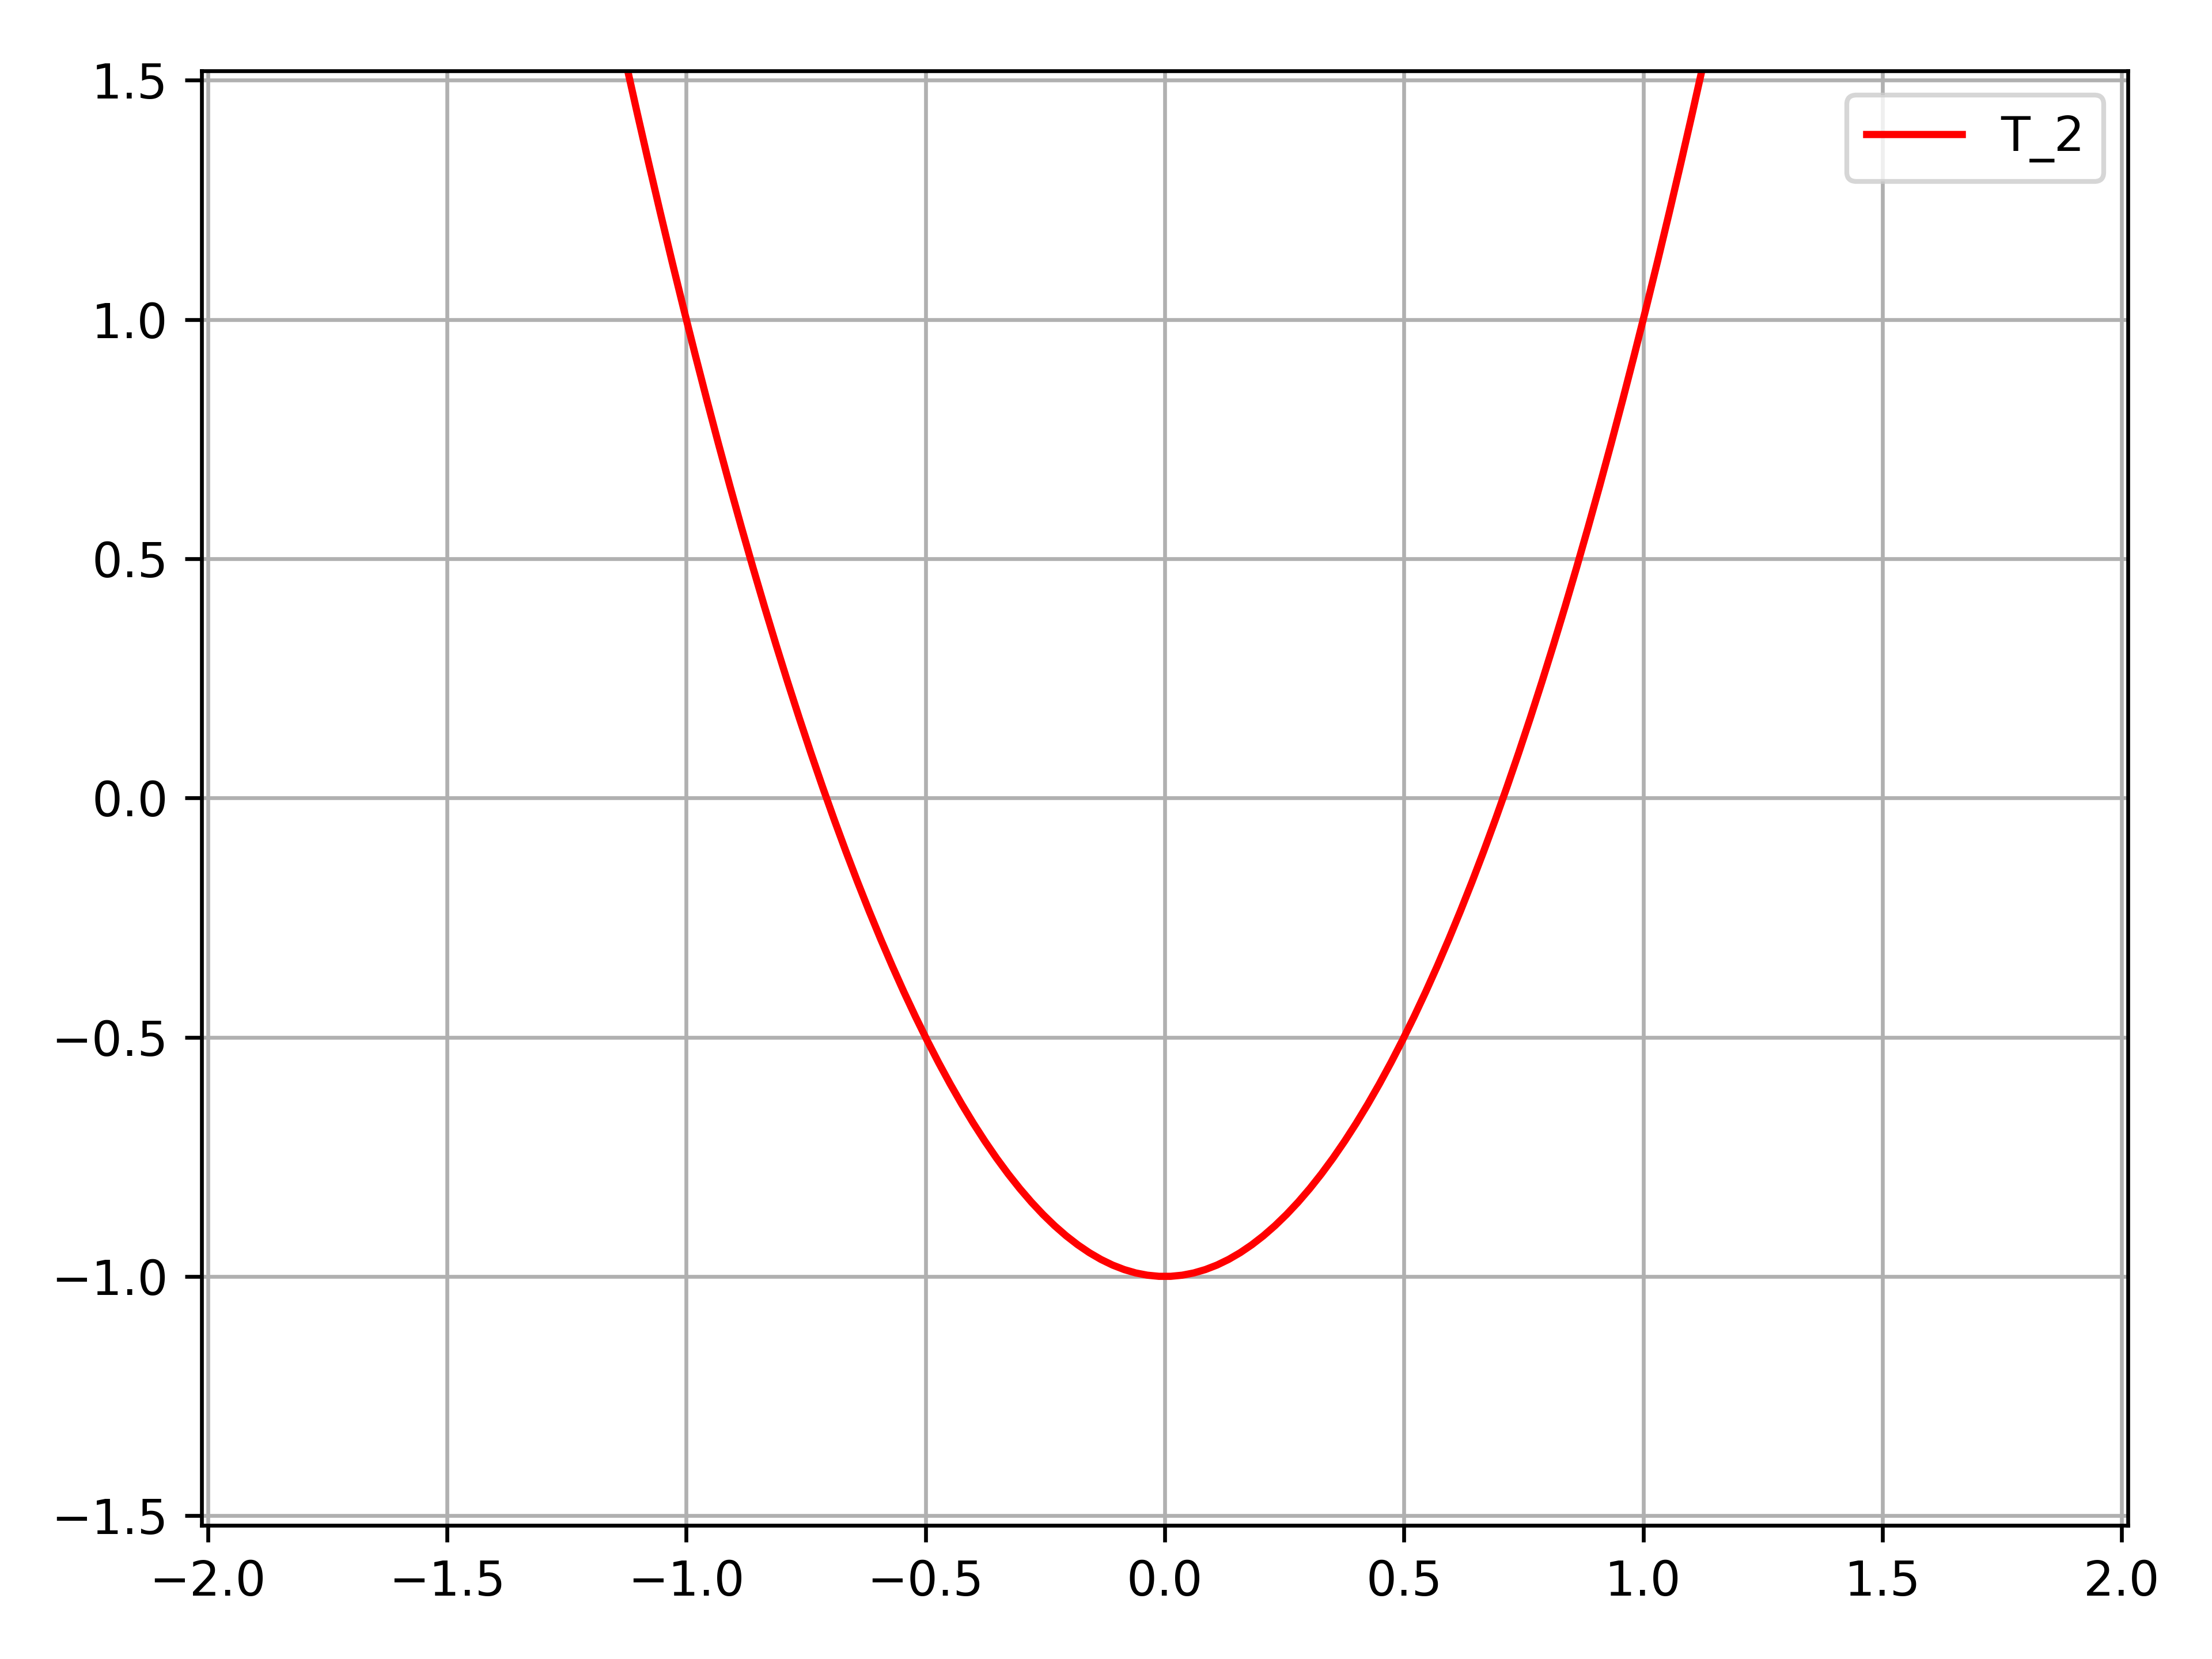
\includegraphics[scale=\myscale,scale=0.3]{figures/approx-tchebychev-01-2} \qquad
  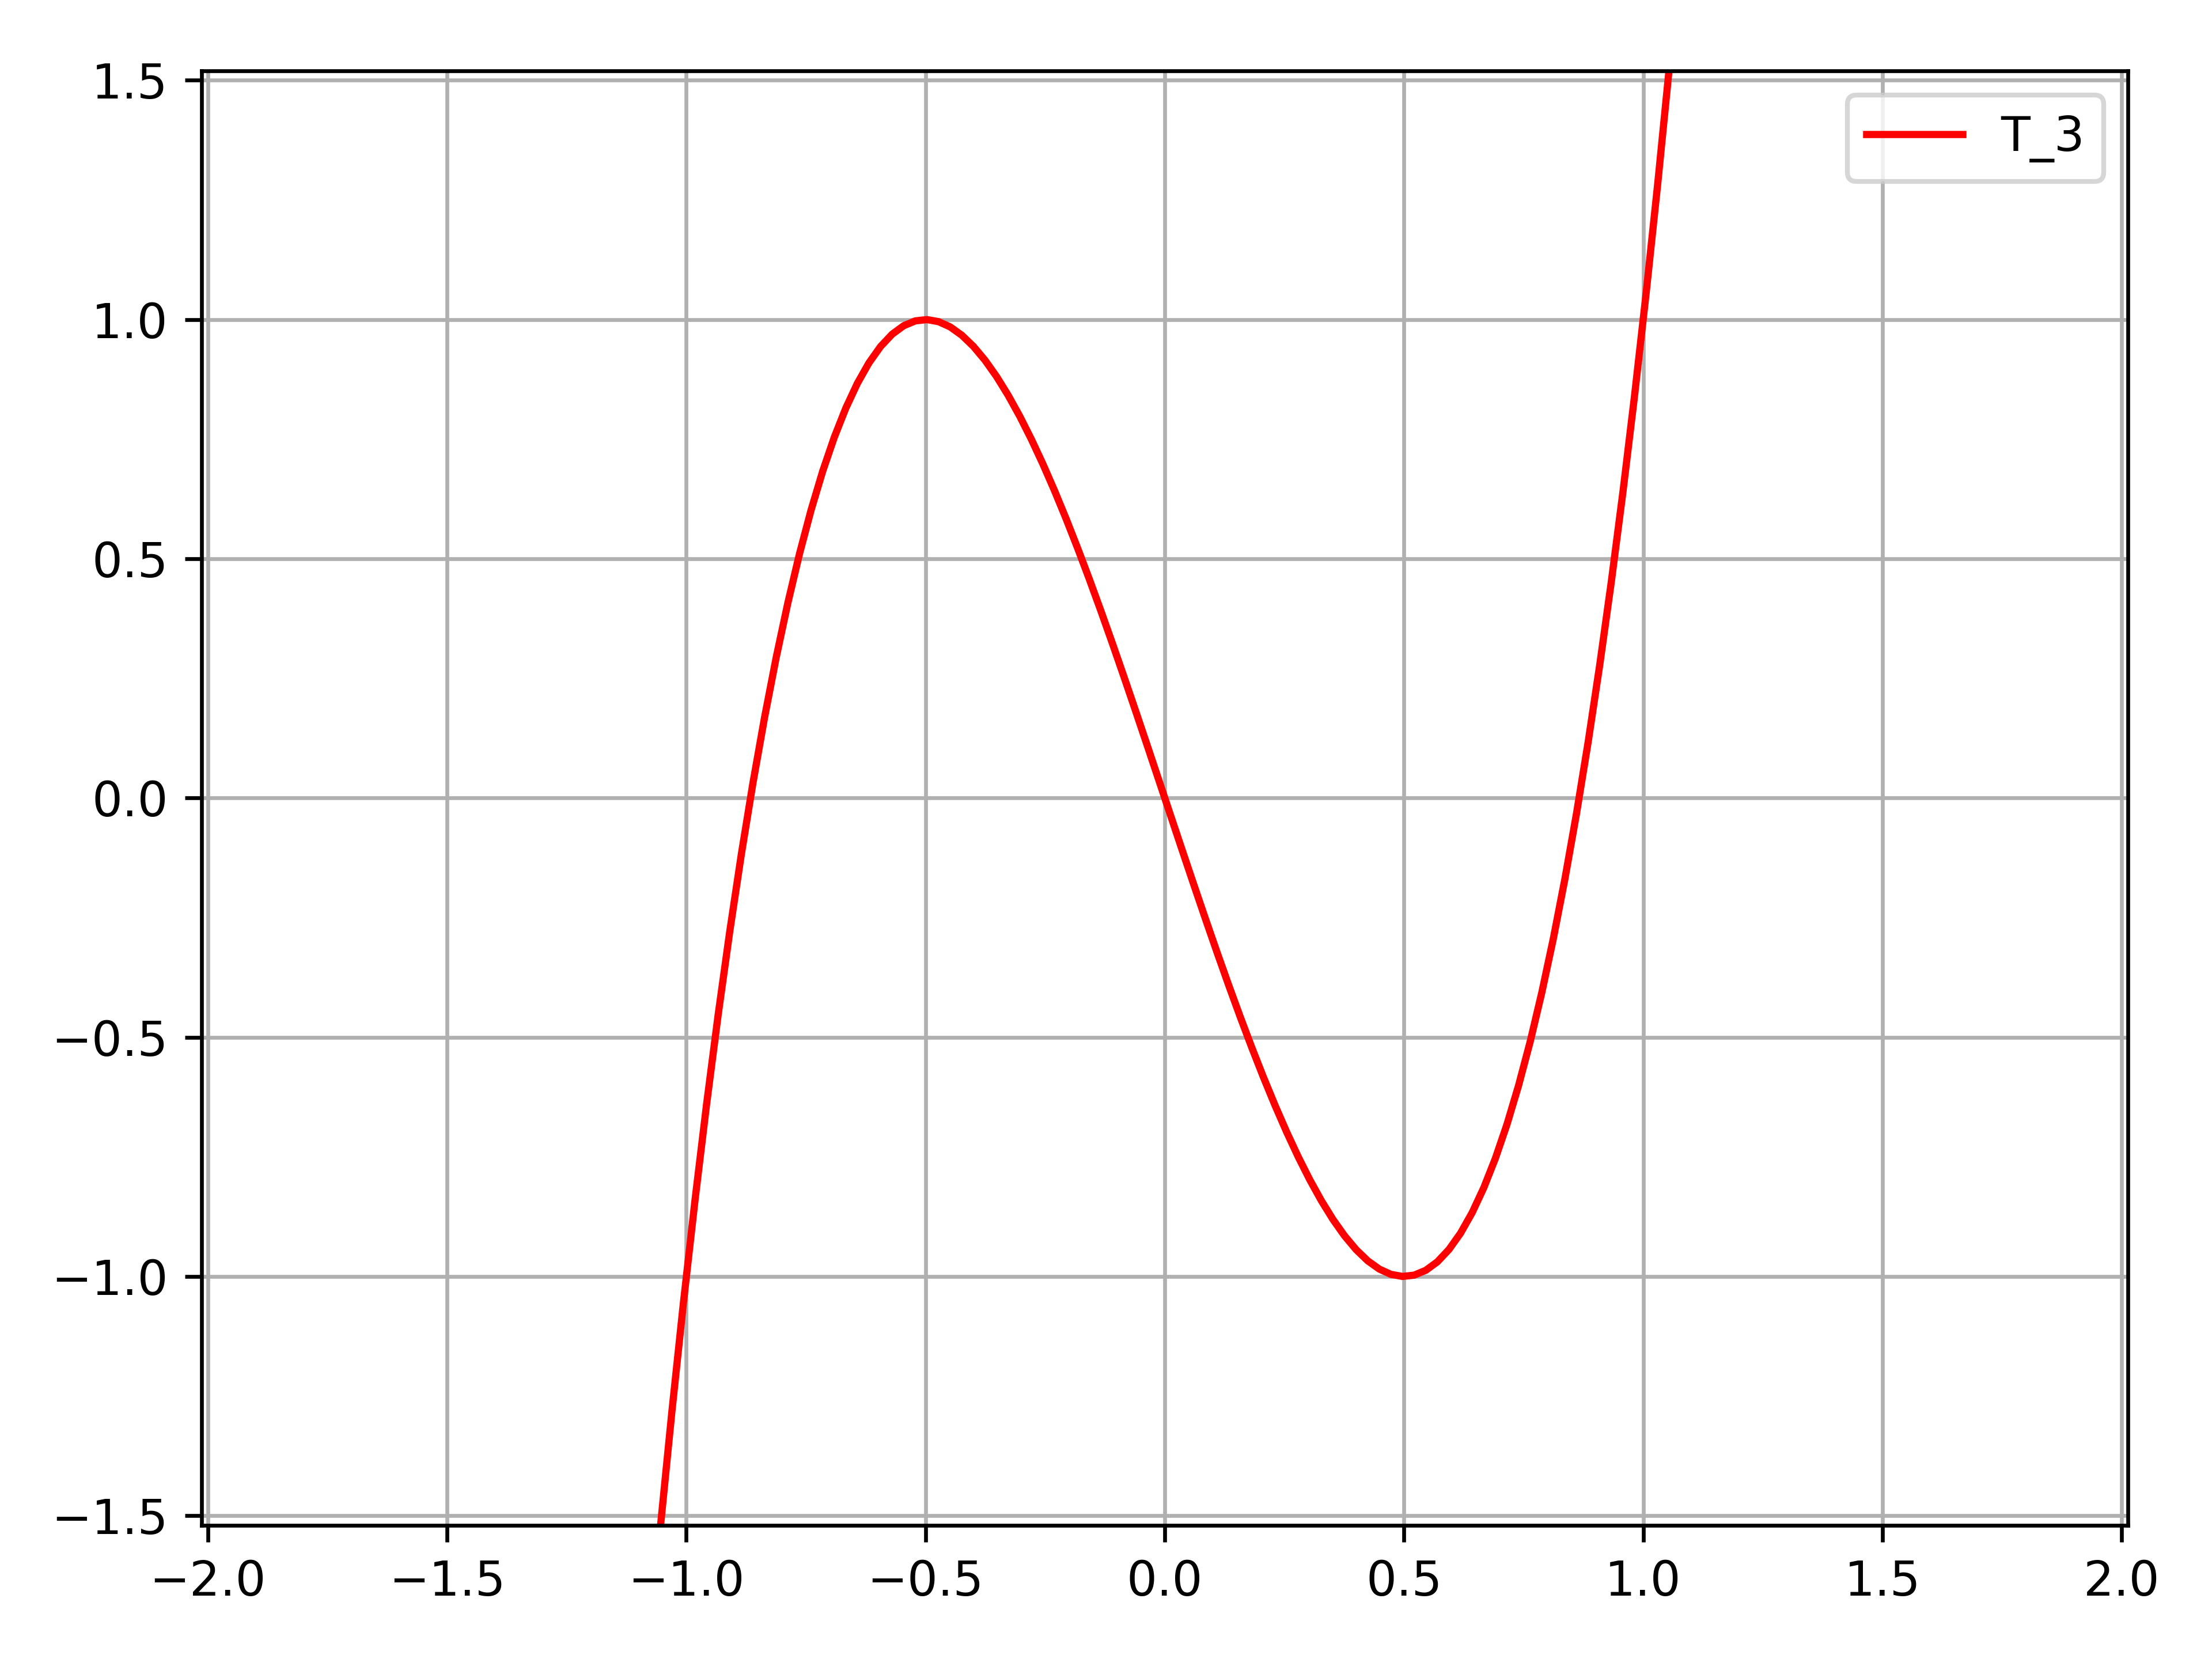
\includegraphics[scale=\myscale,scale=0.3]{figures/approx-tchebychev-01-3}

  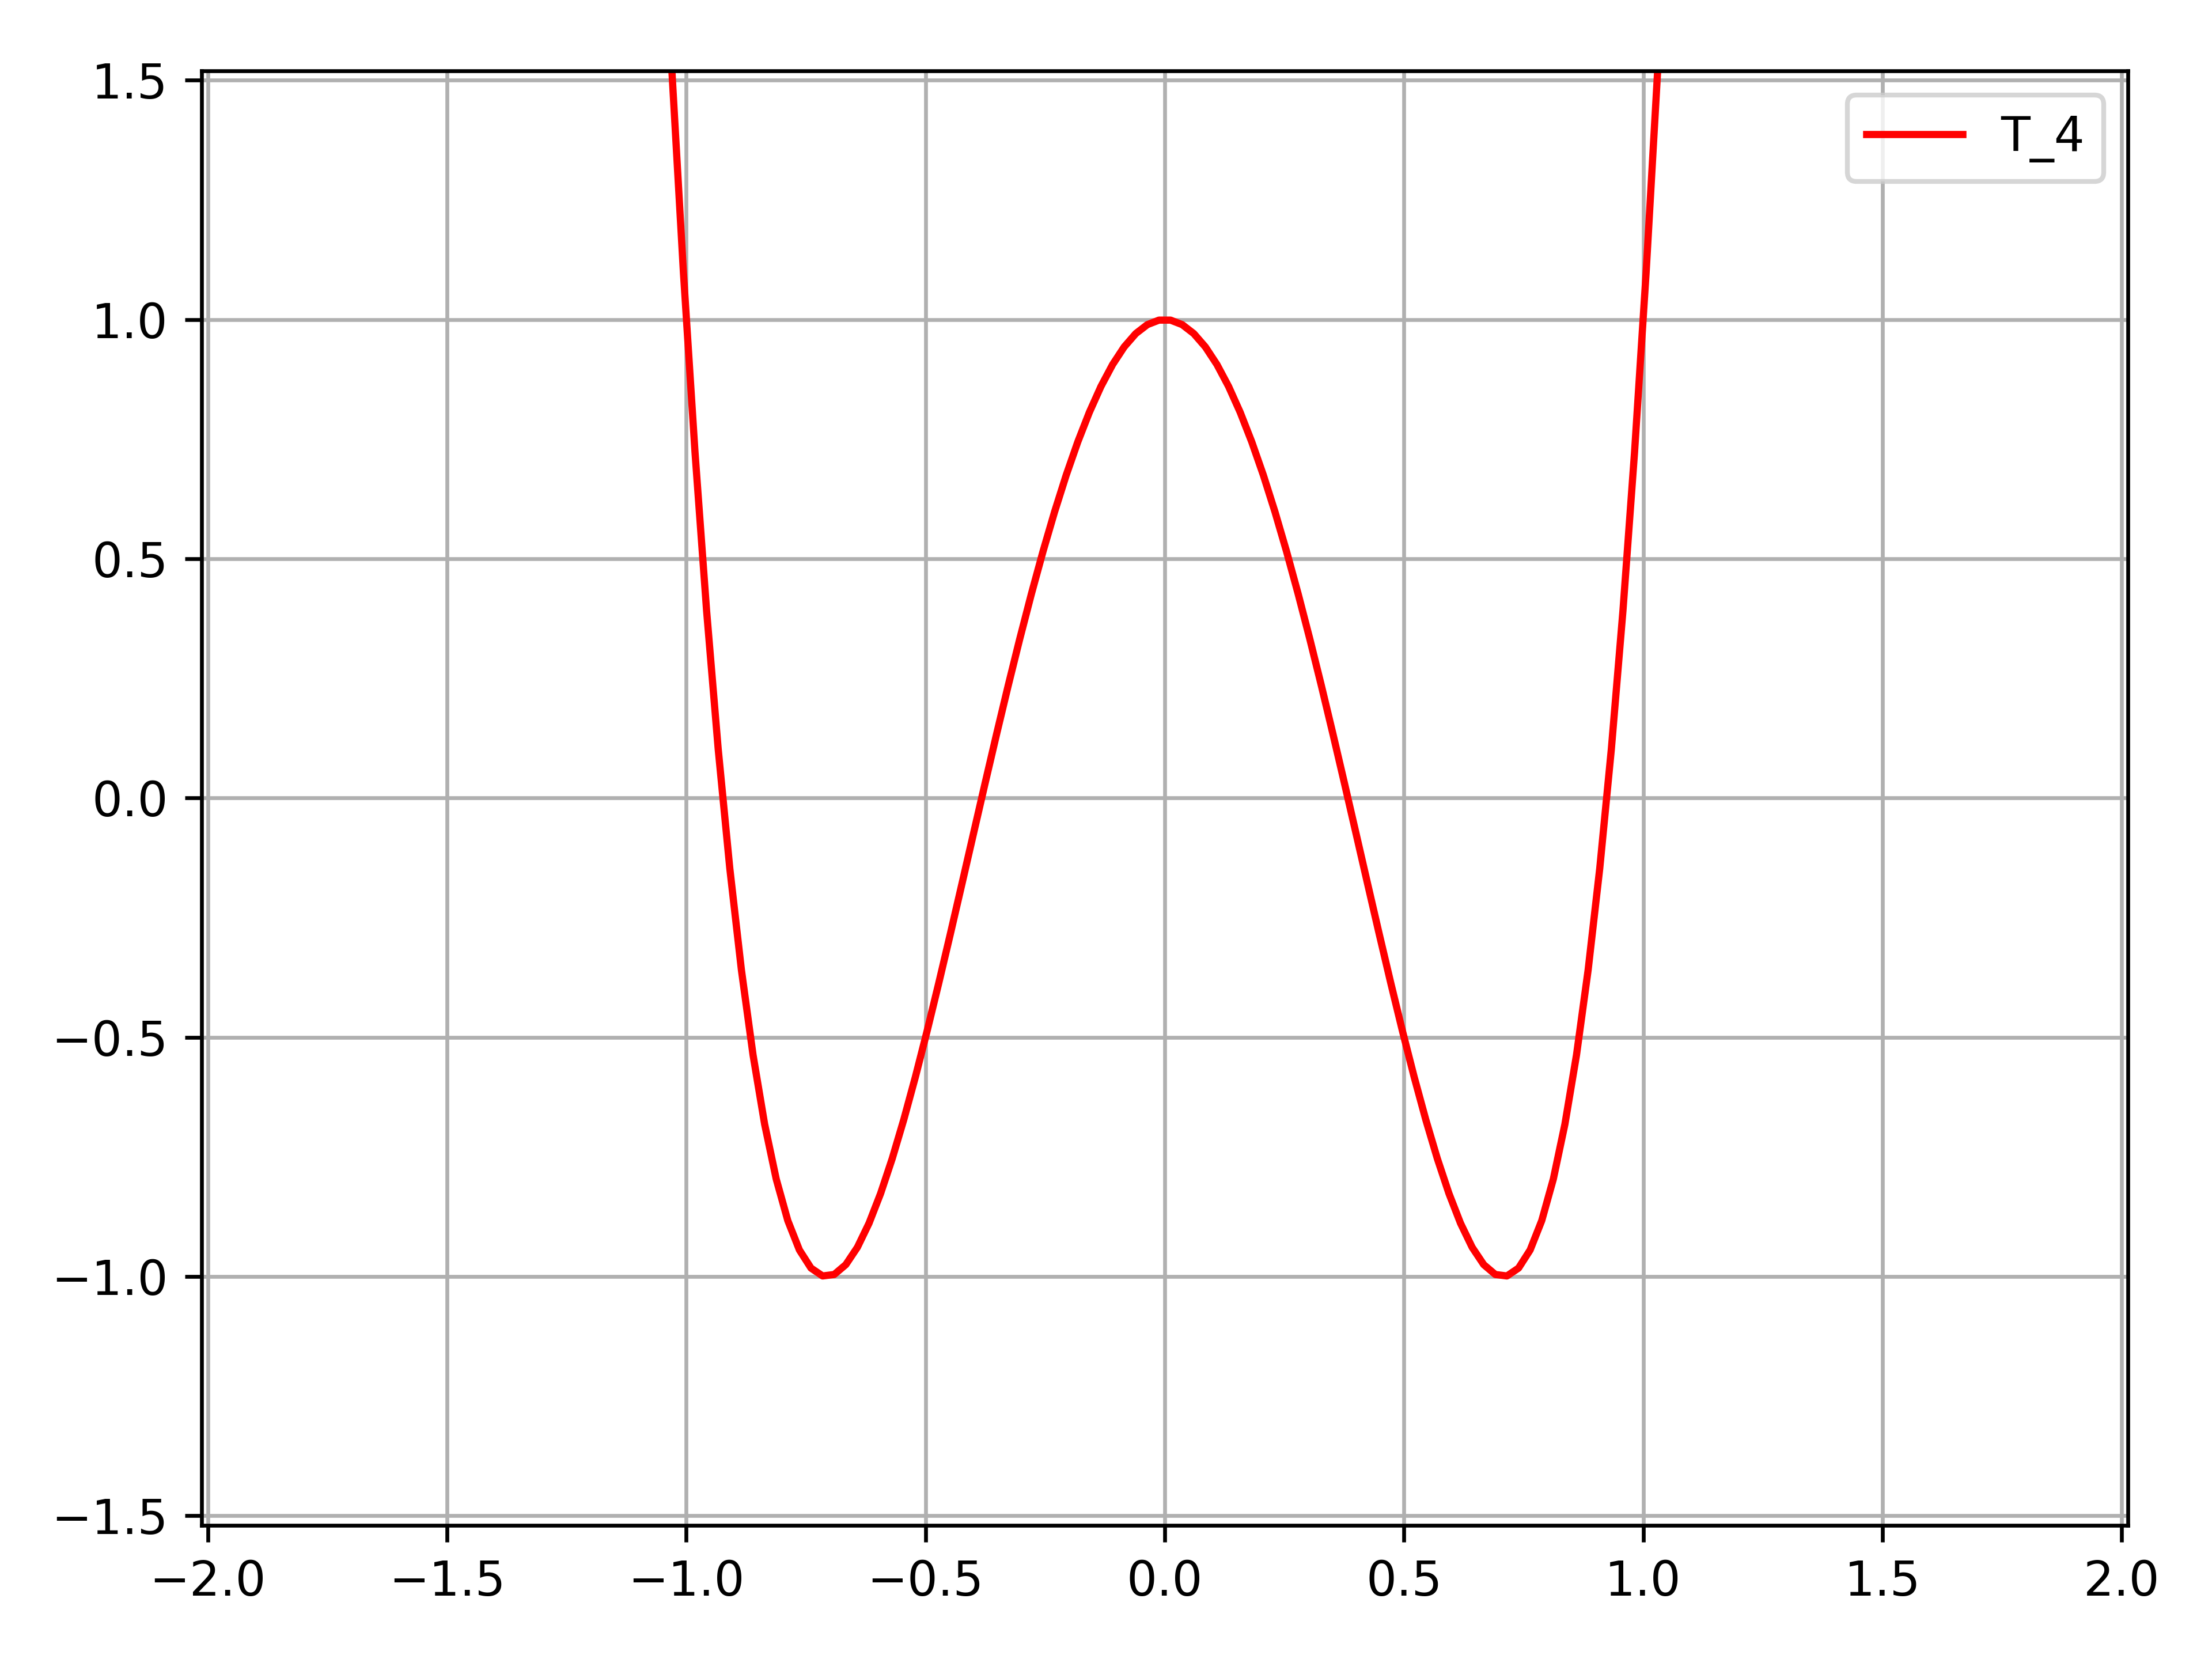
\includegraphics[scale=\myscale,scale=0.3]{figures/approx-tchebychev-01-4} \qquad
  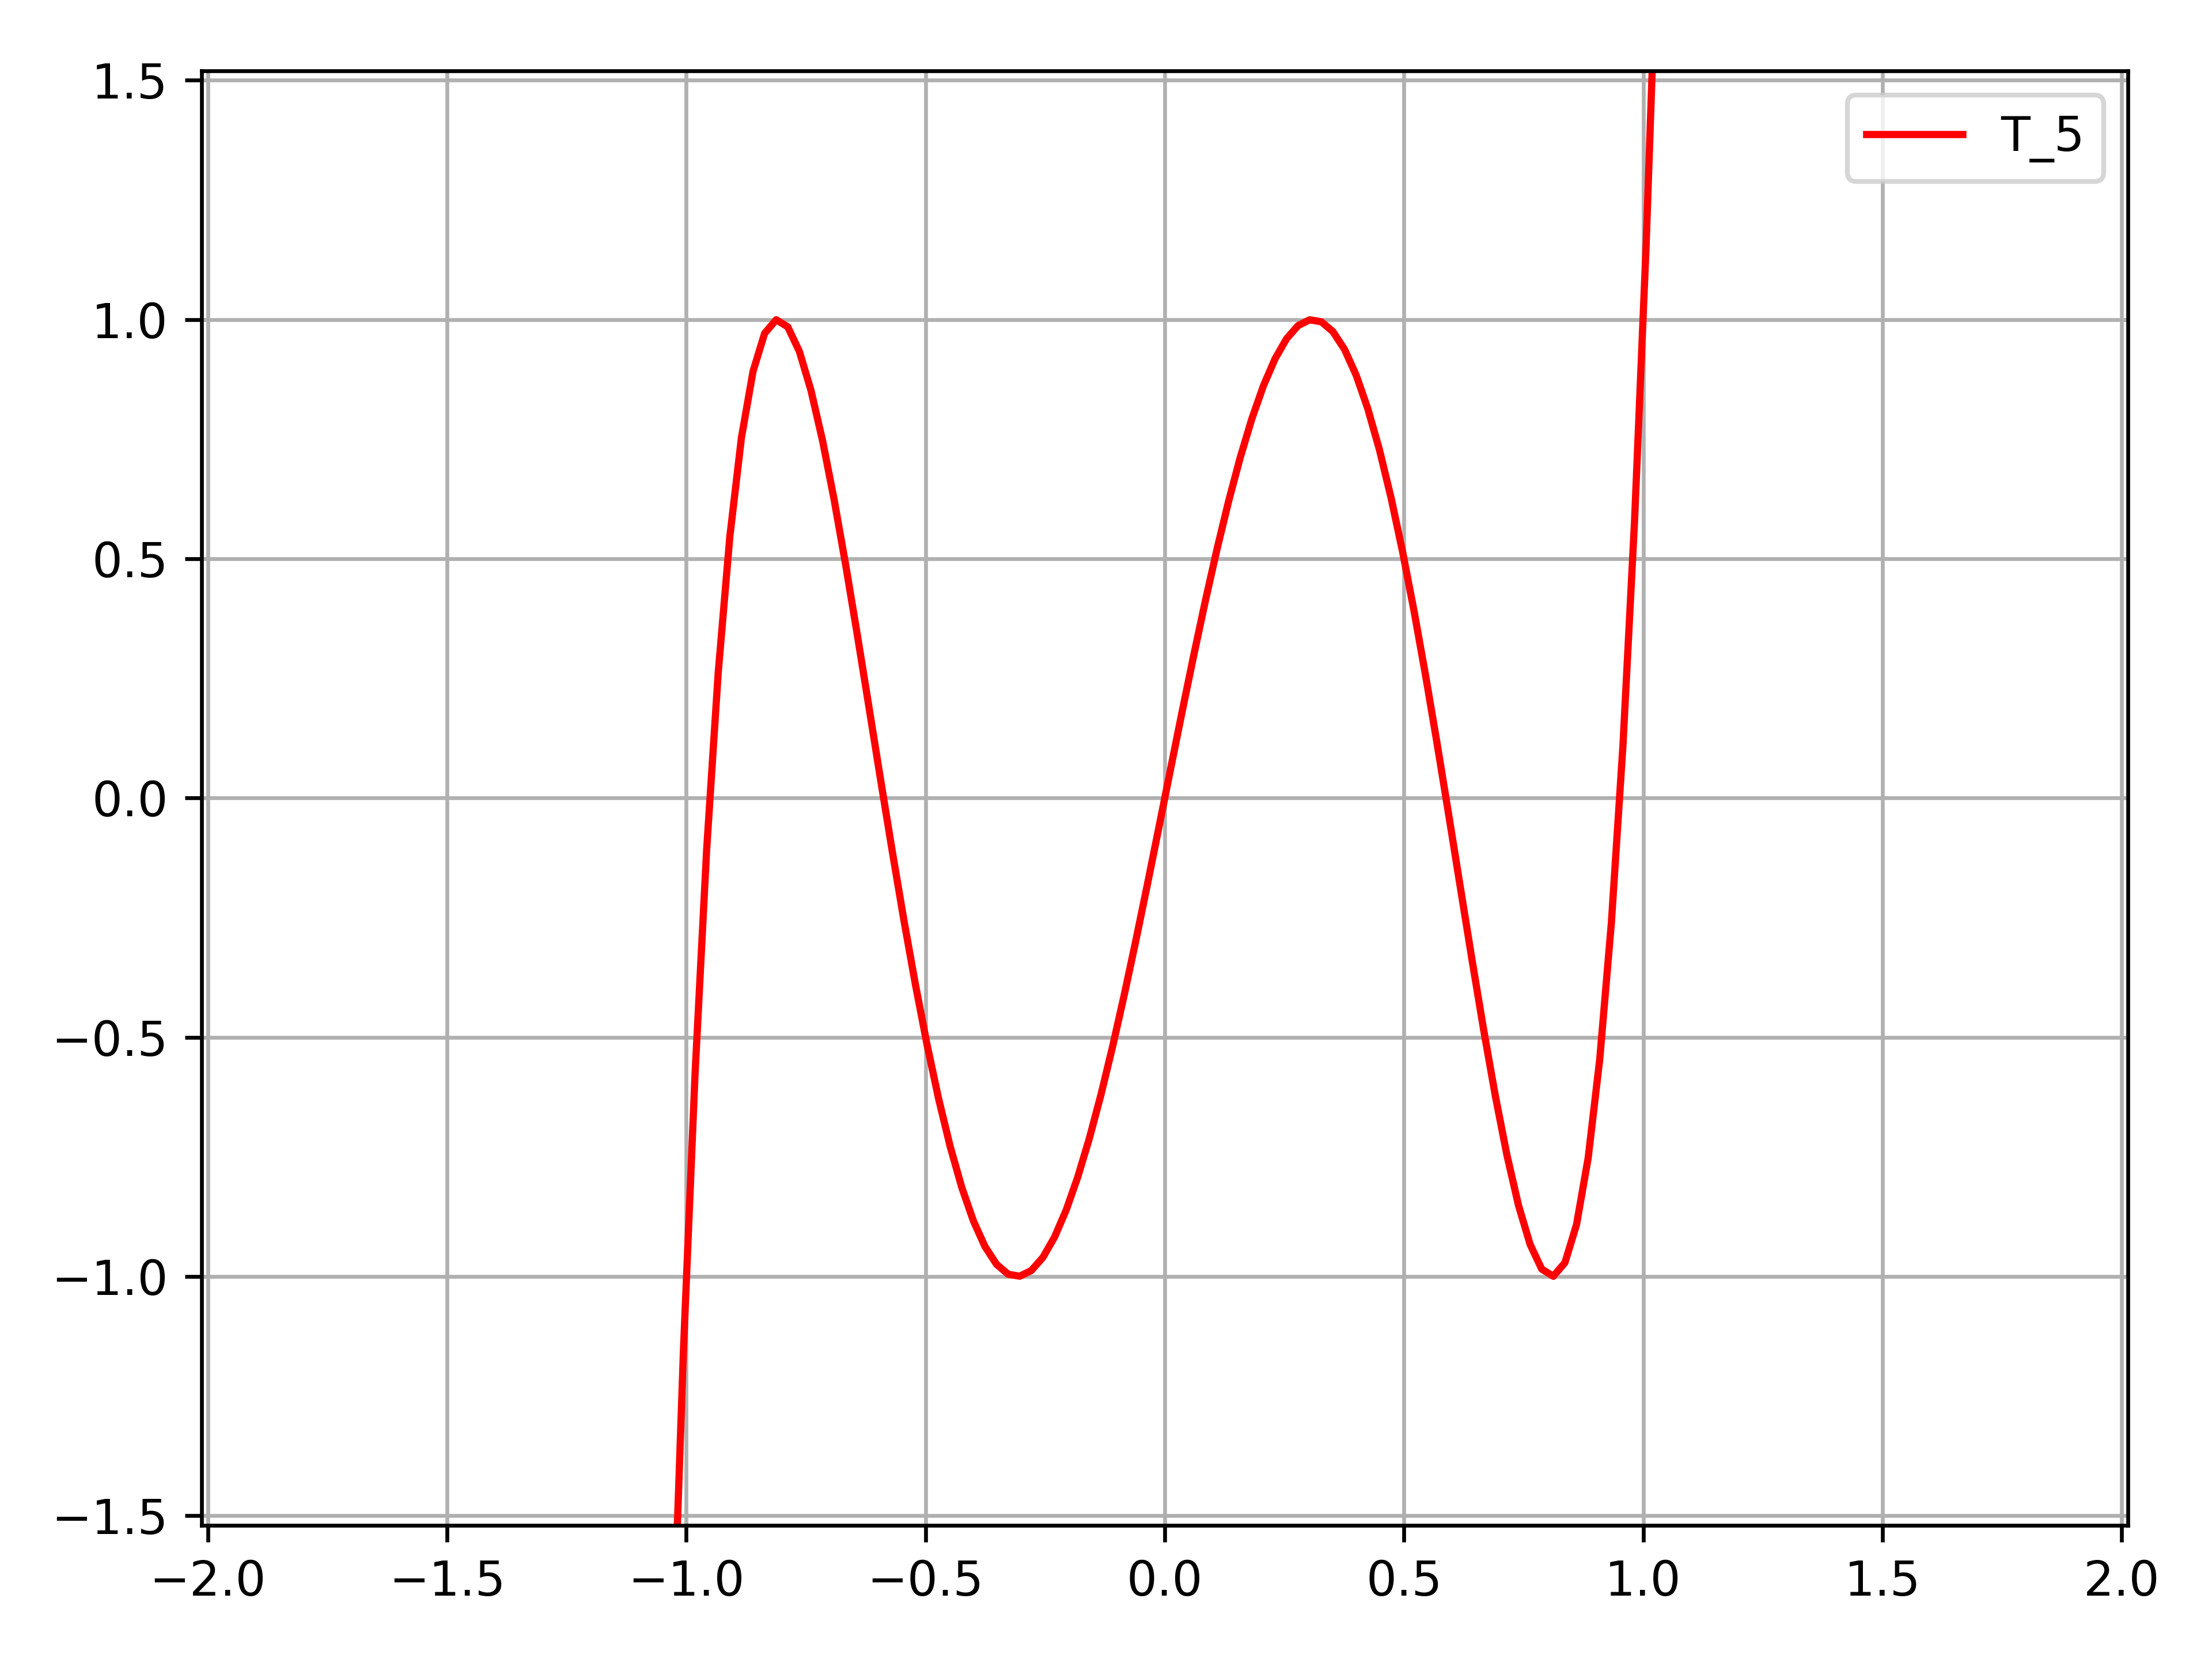
\includegraphics[scale=\myscale,scale=0.3]{figures/approx-tchebychev-01-5} \qquad
  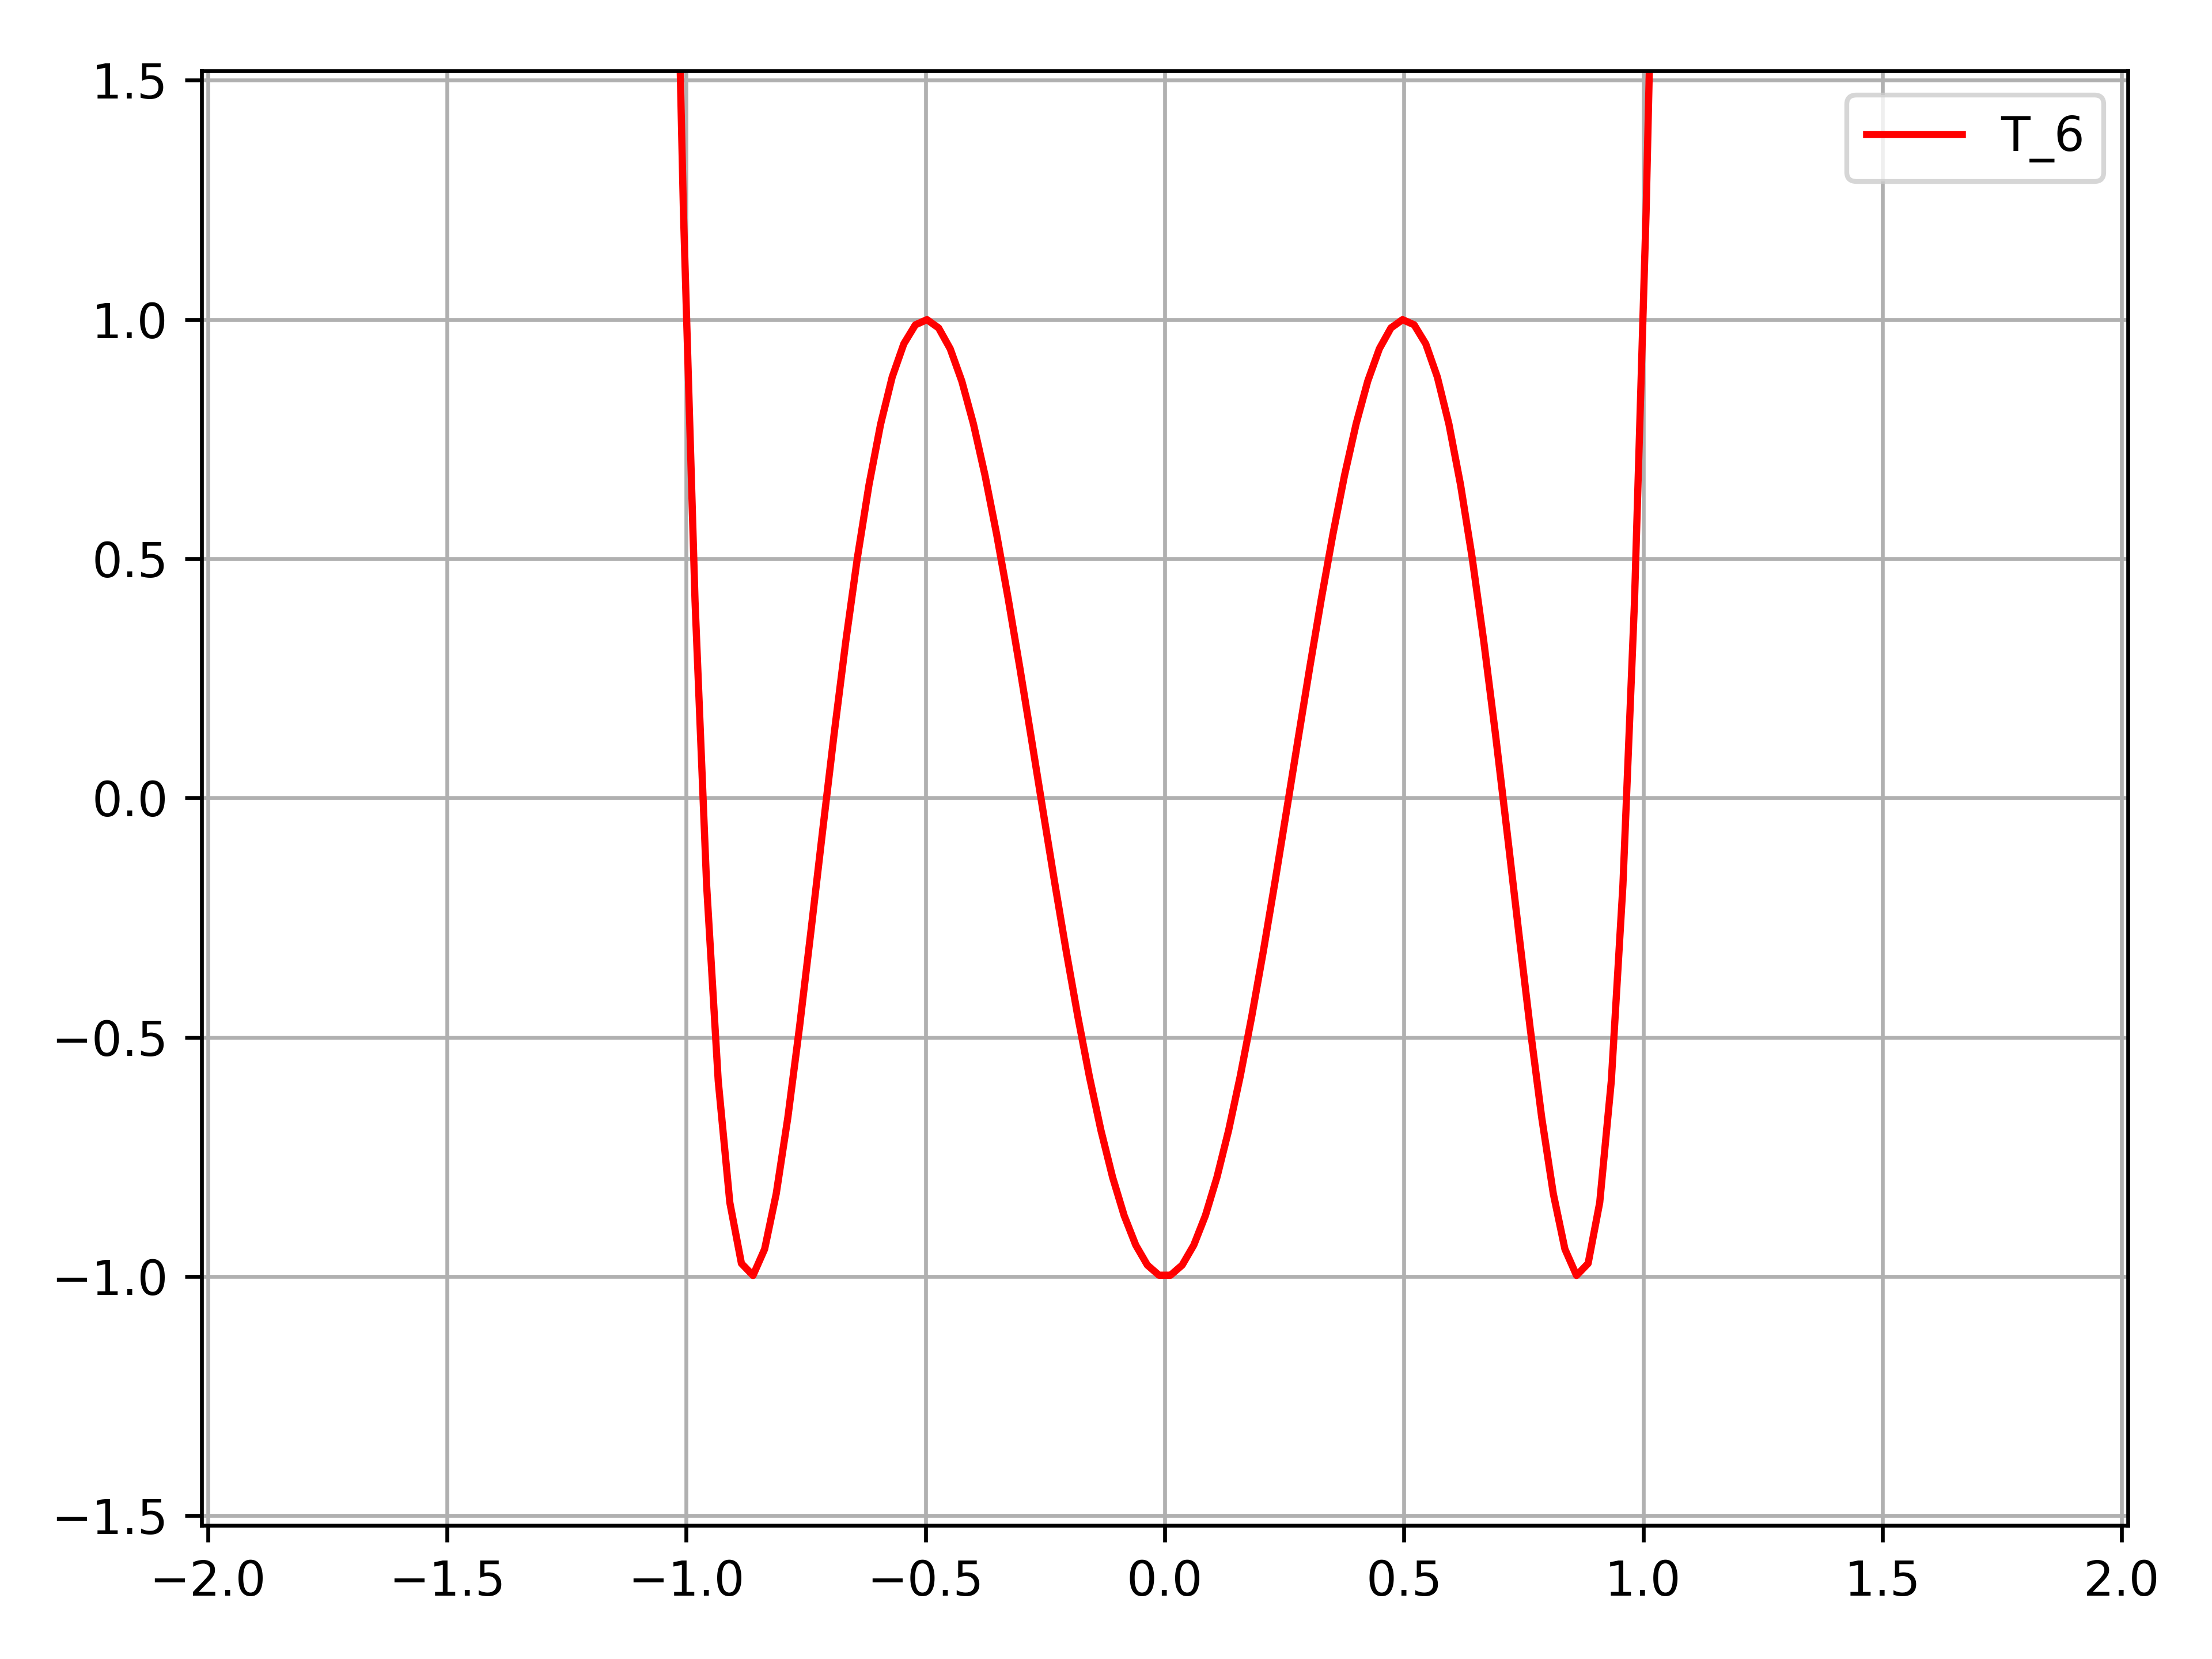
\includegraphics[scale=\myscale,scale=0.3]{figures/approx-tchebychev-01-6} 
\end{center}

Voici quelques propriétés immédiates des polynômes de Tchebychev :
\begin{proposition}
\sauteligne
\begin{itemize}
  \item $T_n(X)$ est un polynôme de degré $n$ de coefficient dominant $2^{n-1}$ (pour tout $n\ge1$).
  \item Le polynôme $T_n(X)$ admet $n$ racines distinctes dans $[-1,1]$ qui sont :
  $$\omega_k = \cos \left(\frac{2k+1}{2n}\pi\right) \qquad k=0,\ldots,n-1.$$
\end{itemize}
\end{proposition}

La propriété qui nous concerne davantage est la suivante :
\begin{proposition}
Le polynôme $\frac{1}{2^{n-1}} T_n(X)$ est le polynôme qui approche au mieux la fonction nulle sur l'intervalle $[-1,1]$ parmi 
tous les polynômes de degré $n$ et de coefficient dominant $1$.
\end{proposition}

La reformulation mathématique de cette proposition est la suivante :
soit $\|f \|_{\infty} = \max_{-1\le x \le 1} |f(x)|$, la norme infinie d'une fonction $f$ sur l'intervalle $[-1,1]$.
Alors $\| T_n \|_{\infty}  = \frac{1}{2^{n-1}}$ est la plus petite norme possible pour un polynôme de degré $n$ et de coefficient dominant $1$.

\begin{center}
  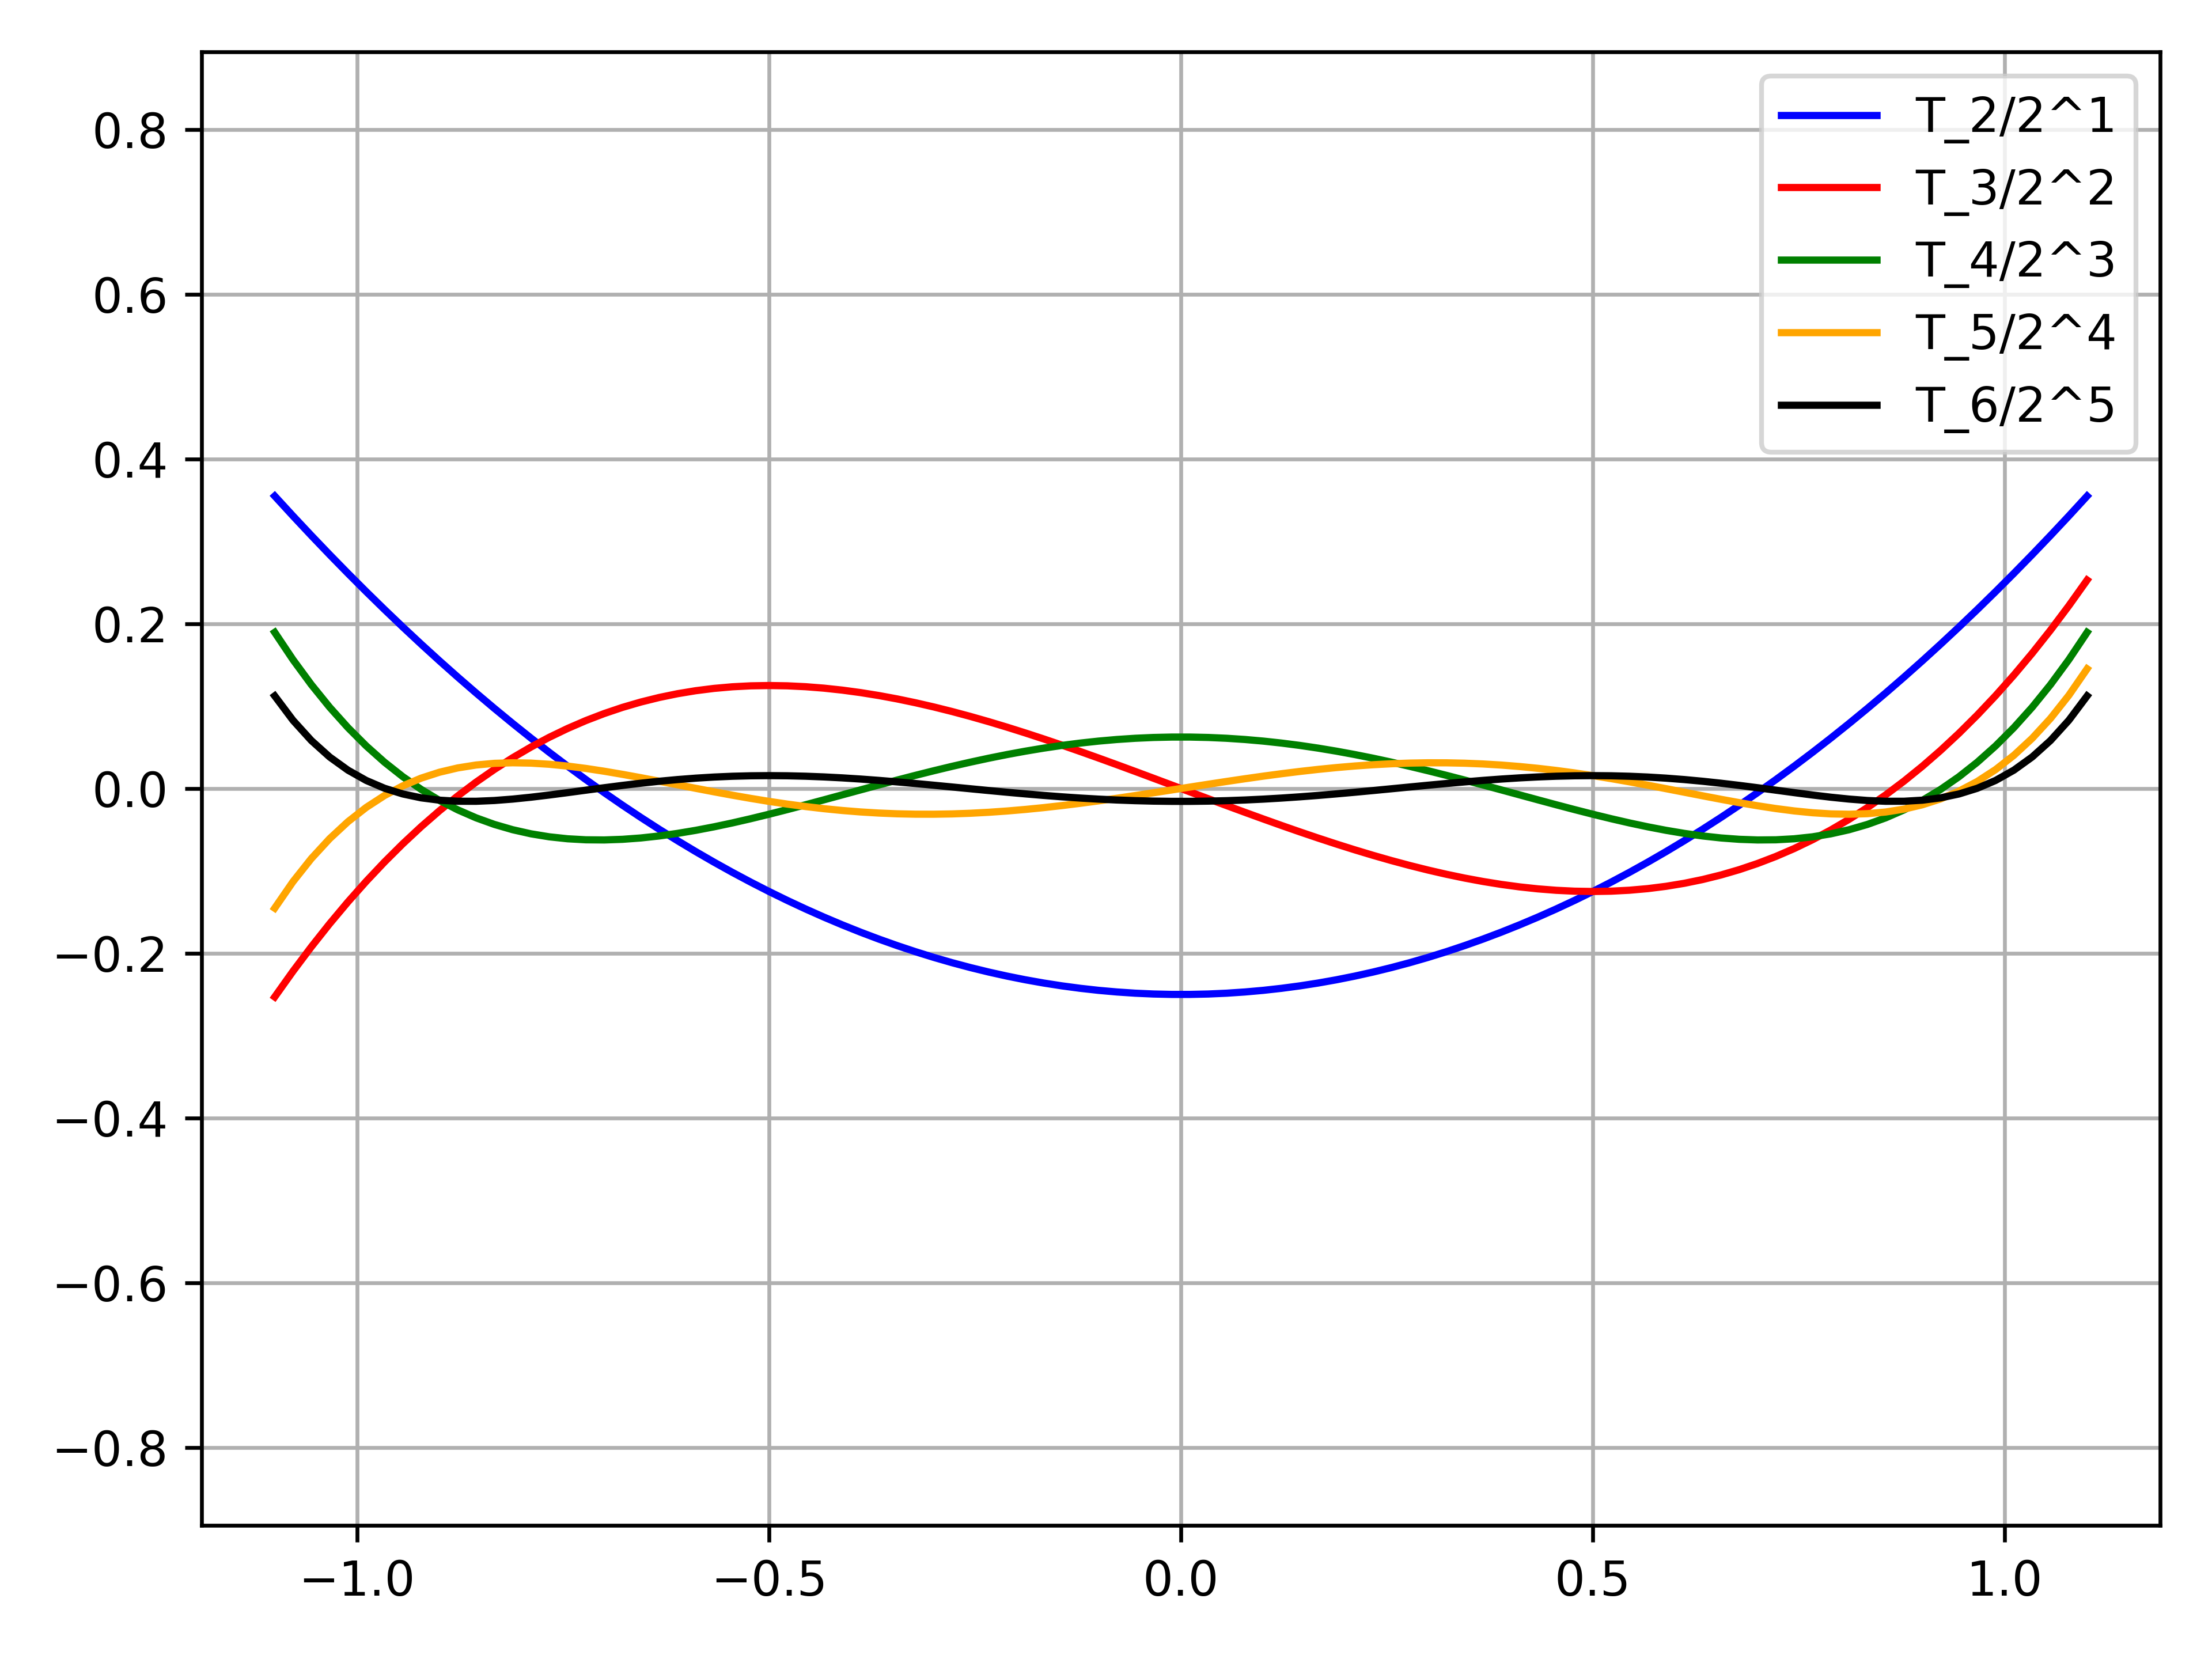
\includegraphics[scale=\myscale,scale=0.6]{figures/approx-tchebychev-02}
\end{center}

Évidemment approcher la fonction nulle a peu d'intérêt en soi mais prouve que les polynômes de Tchebychev permettent 
d'approcher efficacement une fonction sur un intervalle tout entier et pas seulement en quelques points.
Les polynômes de Tchebychev permettent en fait d'approcher n'importe quelle fonction 
sur un intervalle $[a,b]$ par un polynôme de degré $n$ (de façon analogue aux séries de Fourier).
Nous énonçons le résultat de manière informelle. 

Soit $f : [-1,1] \to \Rr$ une fonction continue et dérivable.
Il existe des coefficients $c_i \in \Rr$ tels que $P(X) = \sum_{i=0}^{n-1} c_i T_i(X)$ est un polynôme de degré $n-1$ 
qui approche correctement $f$ sur l'intervalle $[-1,1]$ :
\mybox{$\displaystyle f(x) \simeq \sum_{i=0}^{n-1} c_i T_i(x) \qquad \text{ pour tout } x \in [-1,1]$}
où les coefficients se calculent par les formules :
\mybox{$\displaystyle 
c_0 = \frac{1}{n} \sum_{k=0}^{n-1} f(\omega_k)  \qquad \text{ et } \qquad 
c_i = \frac{2}{n} \sum_{k=0}^{n-1} f(\omega_k) T_i(\omega_k) \quad \text{ pour } i=1,\ldots,n-1
$}
et où les $\omega_k$ sont les $n$ racines de $T_n(X)$.

L'erreur que l'on cherche à minimiser est $\| f - P \|_{\infty}$. Les polynômes de Tchebychev ne fournissent pas une approximation optimale mais
une approximation qui est suffisamment bonne pour être utilisée dans la plupart des cas.

\begin{exemple}
Voici les approximations de la fonction $f(x) = \frac{1}{1+2x+5x^2}$ par des séries de Tchebychev pour les ordres $n=3,5,7,9$.
\begin{center}
  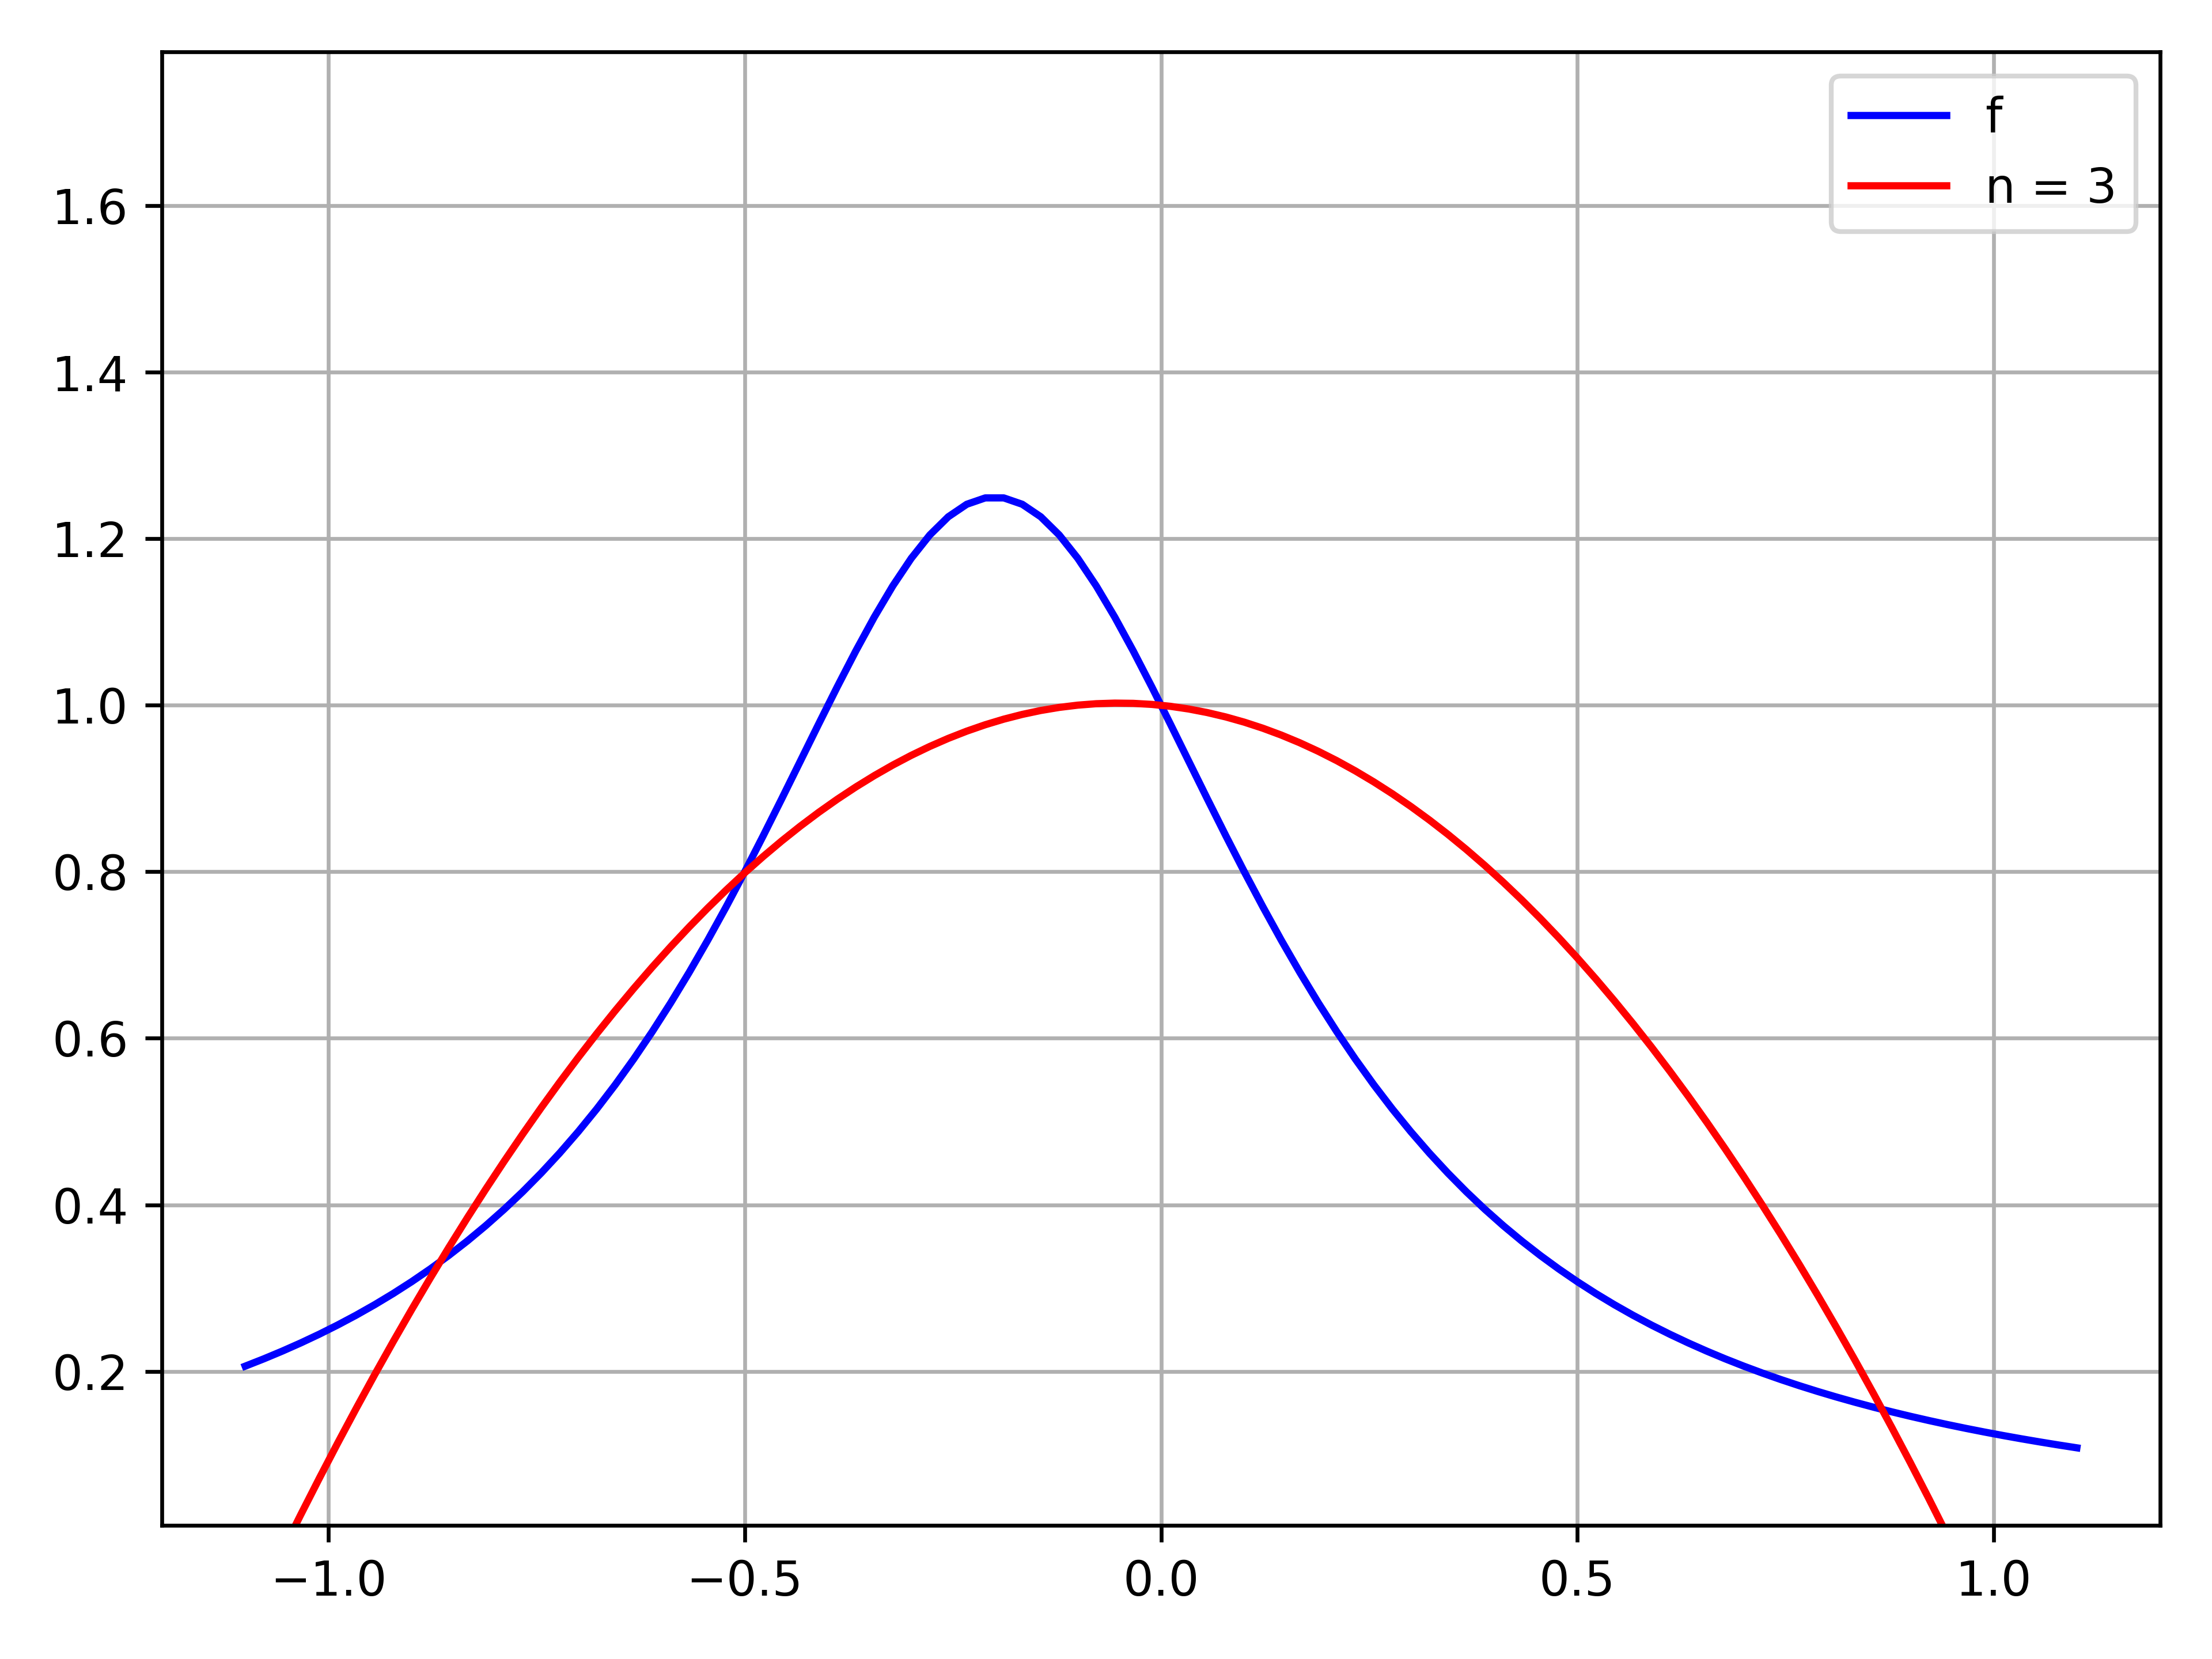
\includegraphics[scale=\myscale,scale=0.45]{figures/approx-tchebychev-03-3} \qquad
  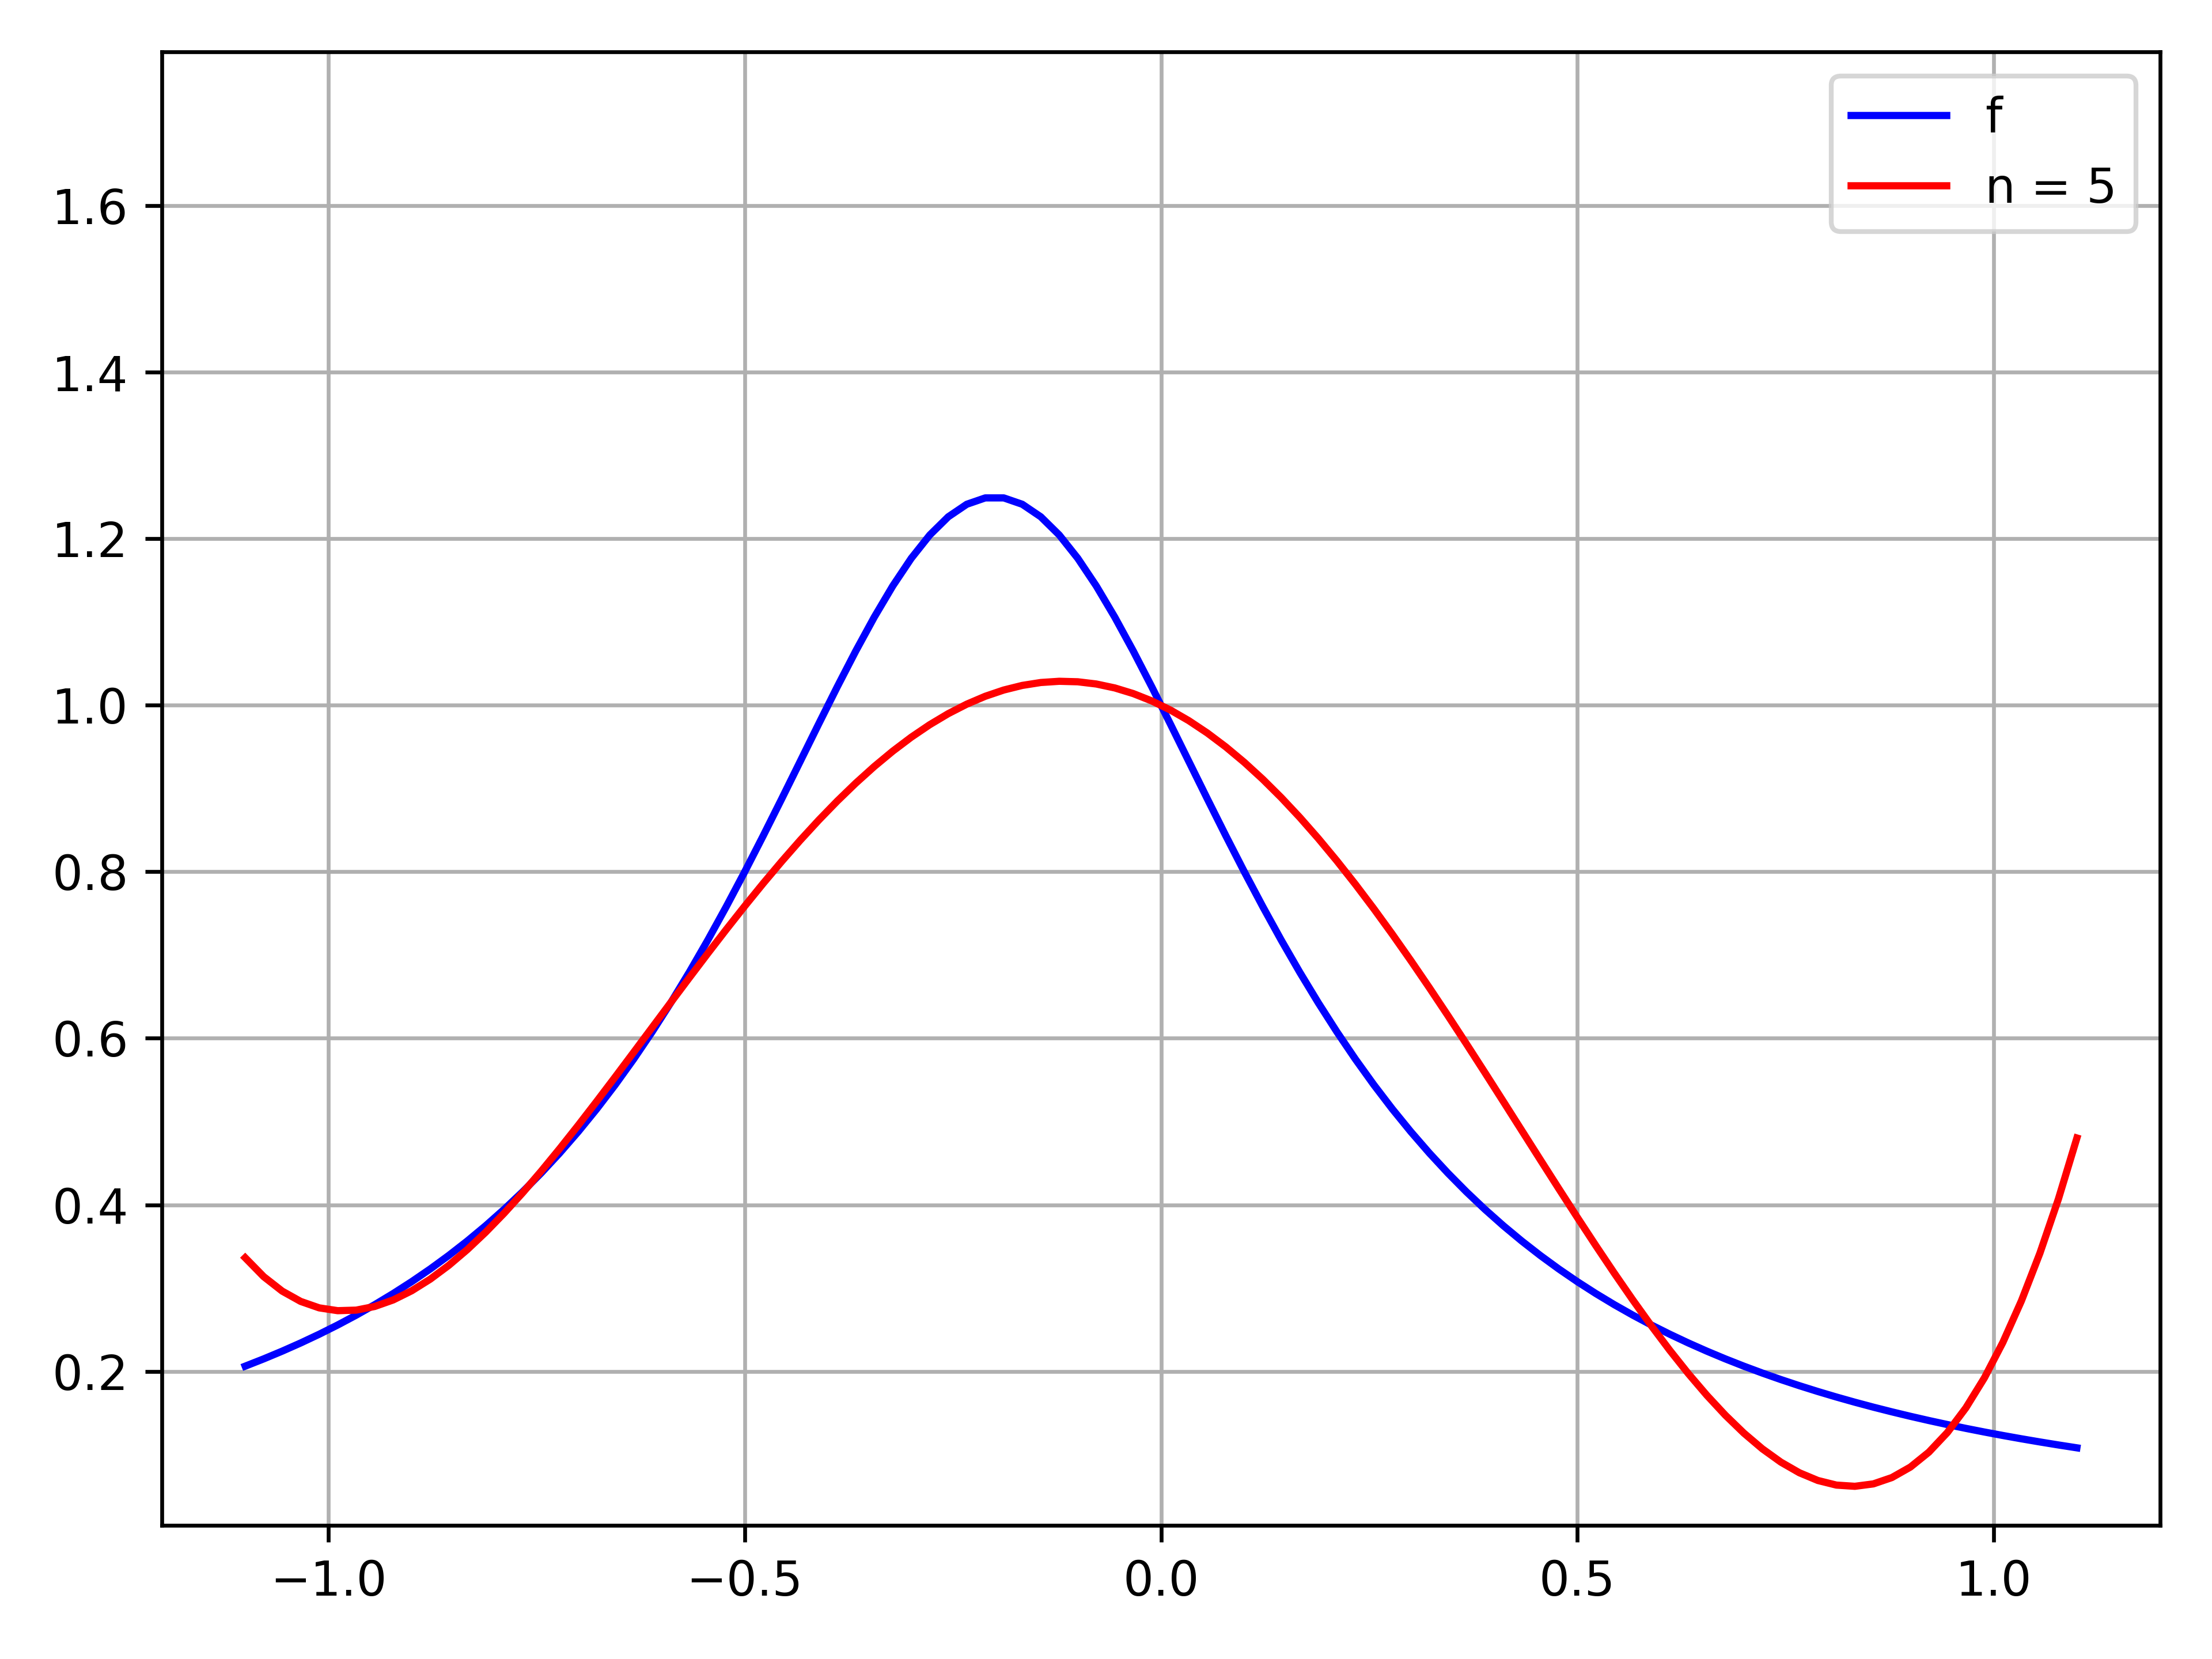
\includegraphics[scale=\myscale,scale=0.45]{figures/approx-tchebychev-03-5} 

  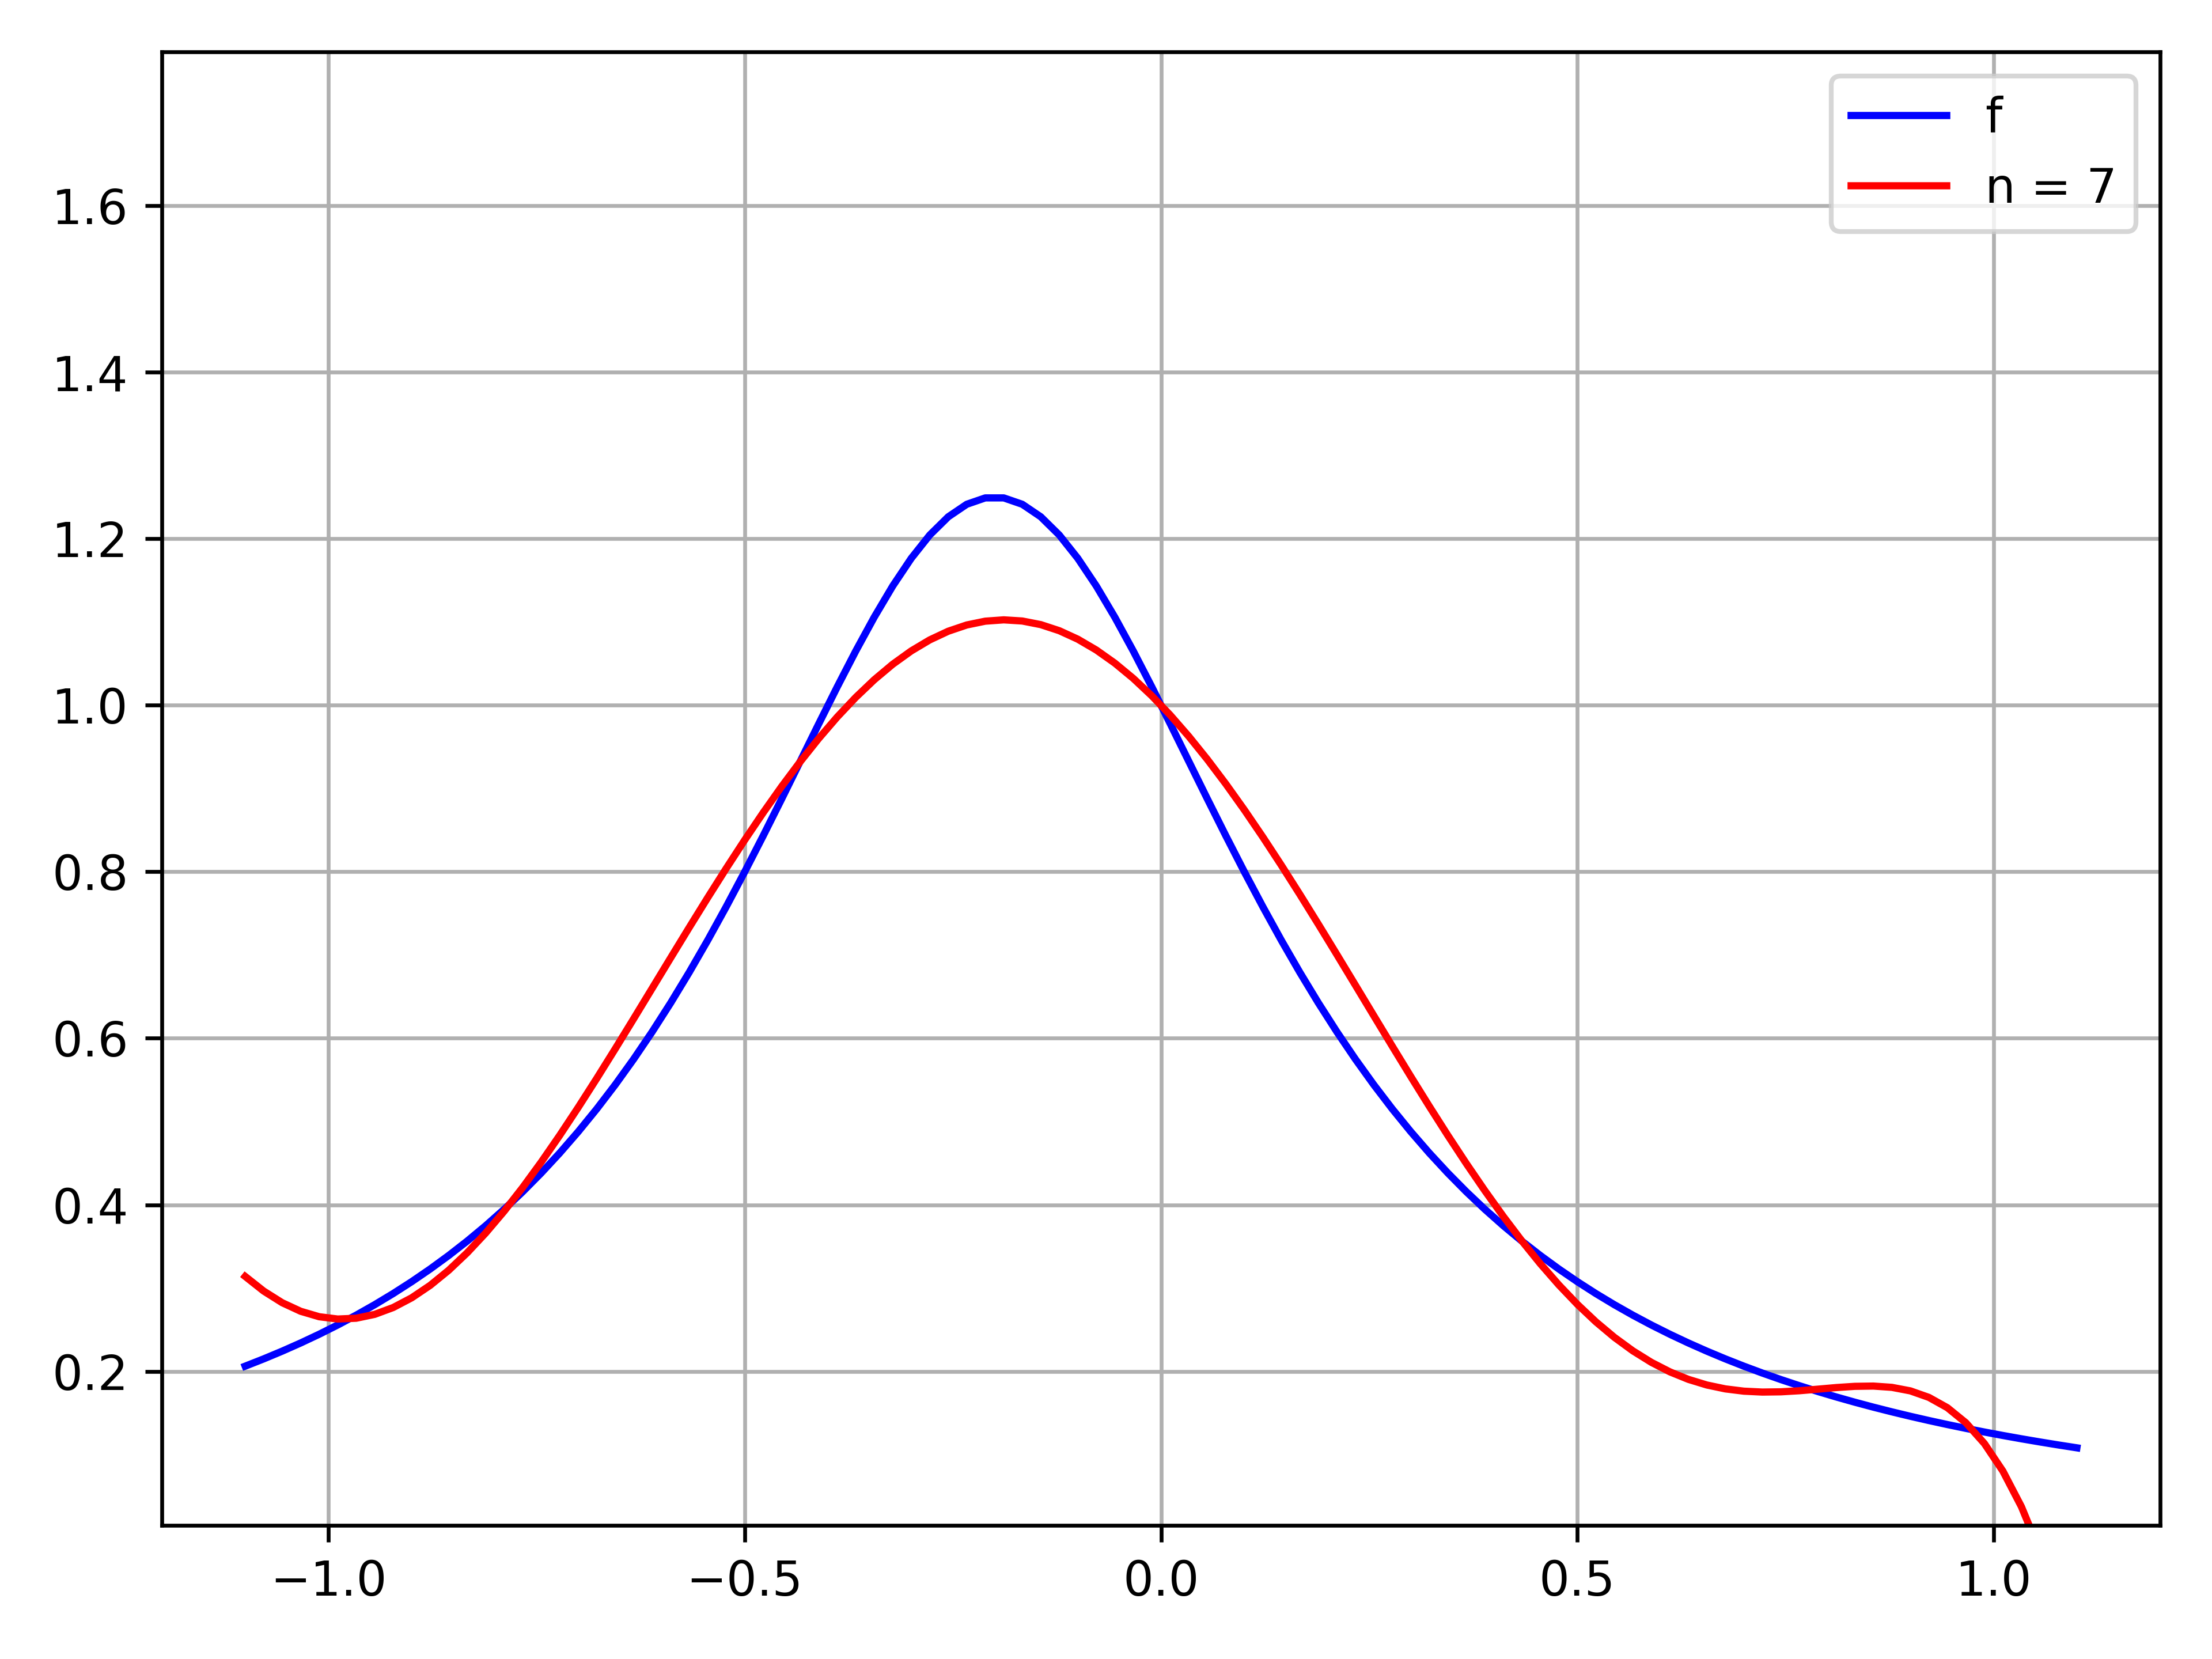
\includegraphics[scale=\myscale,scale=0.45]{figures/approx-tchebychev-03-7} \qquad
  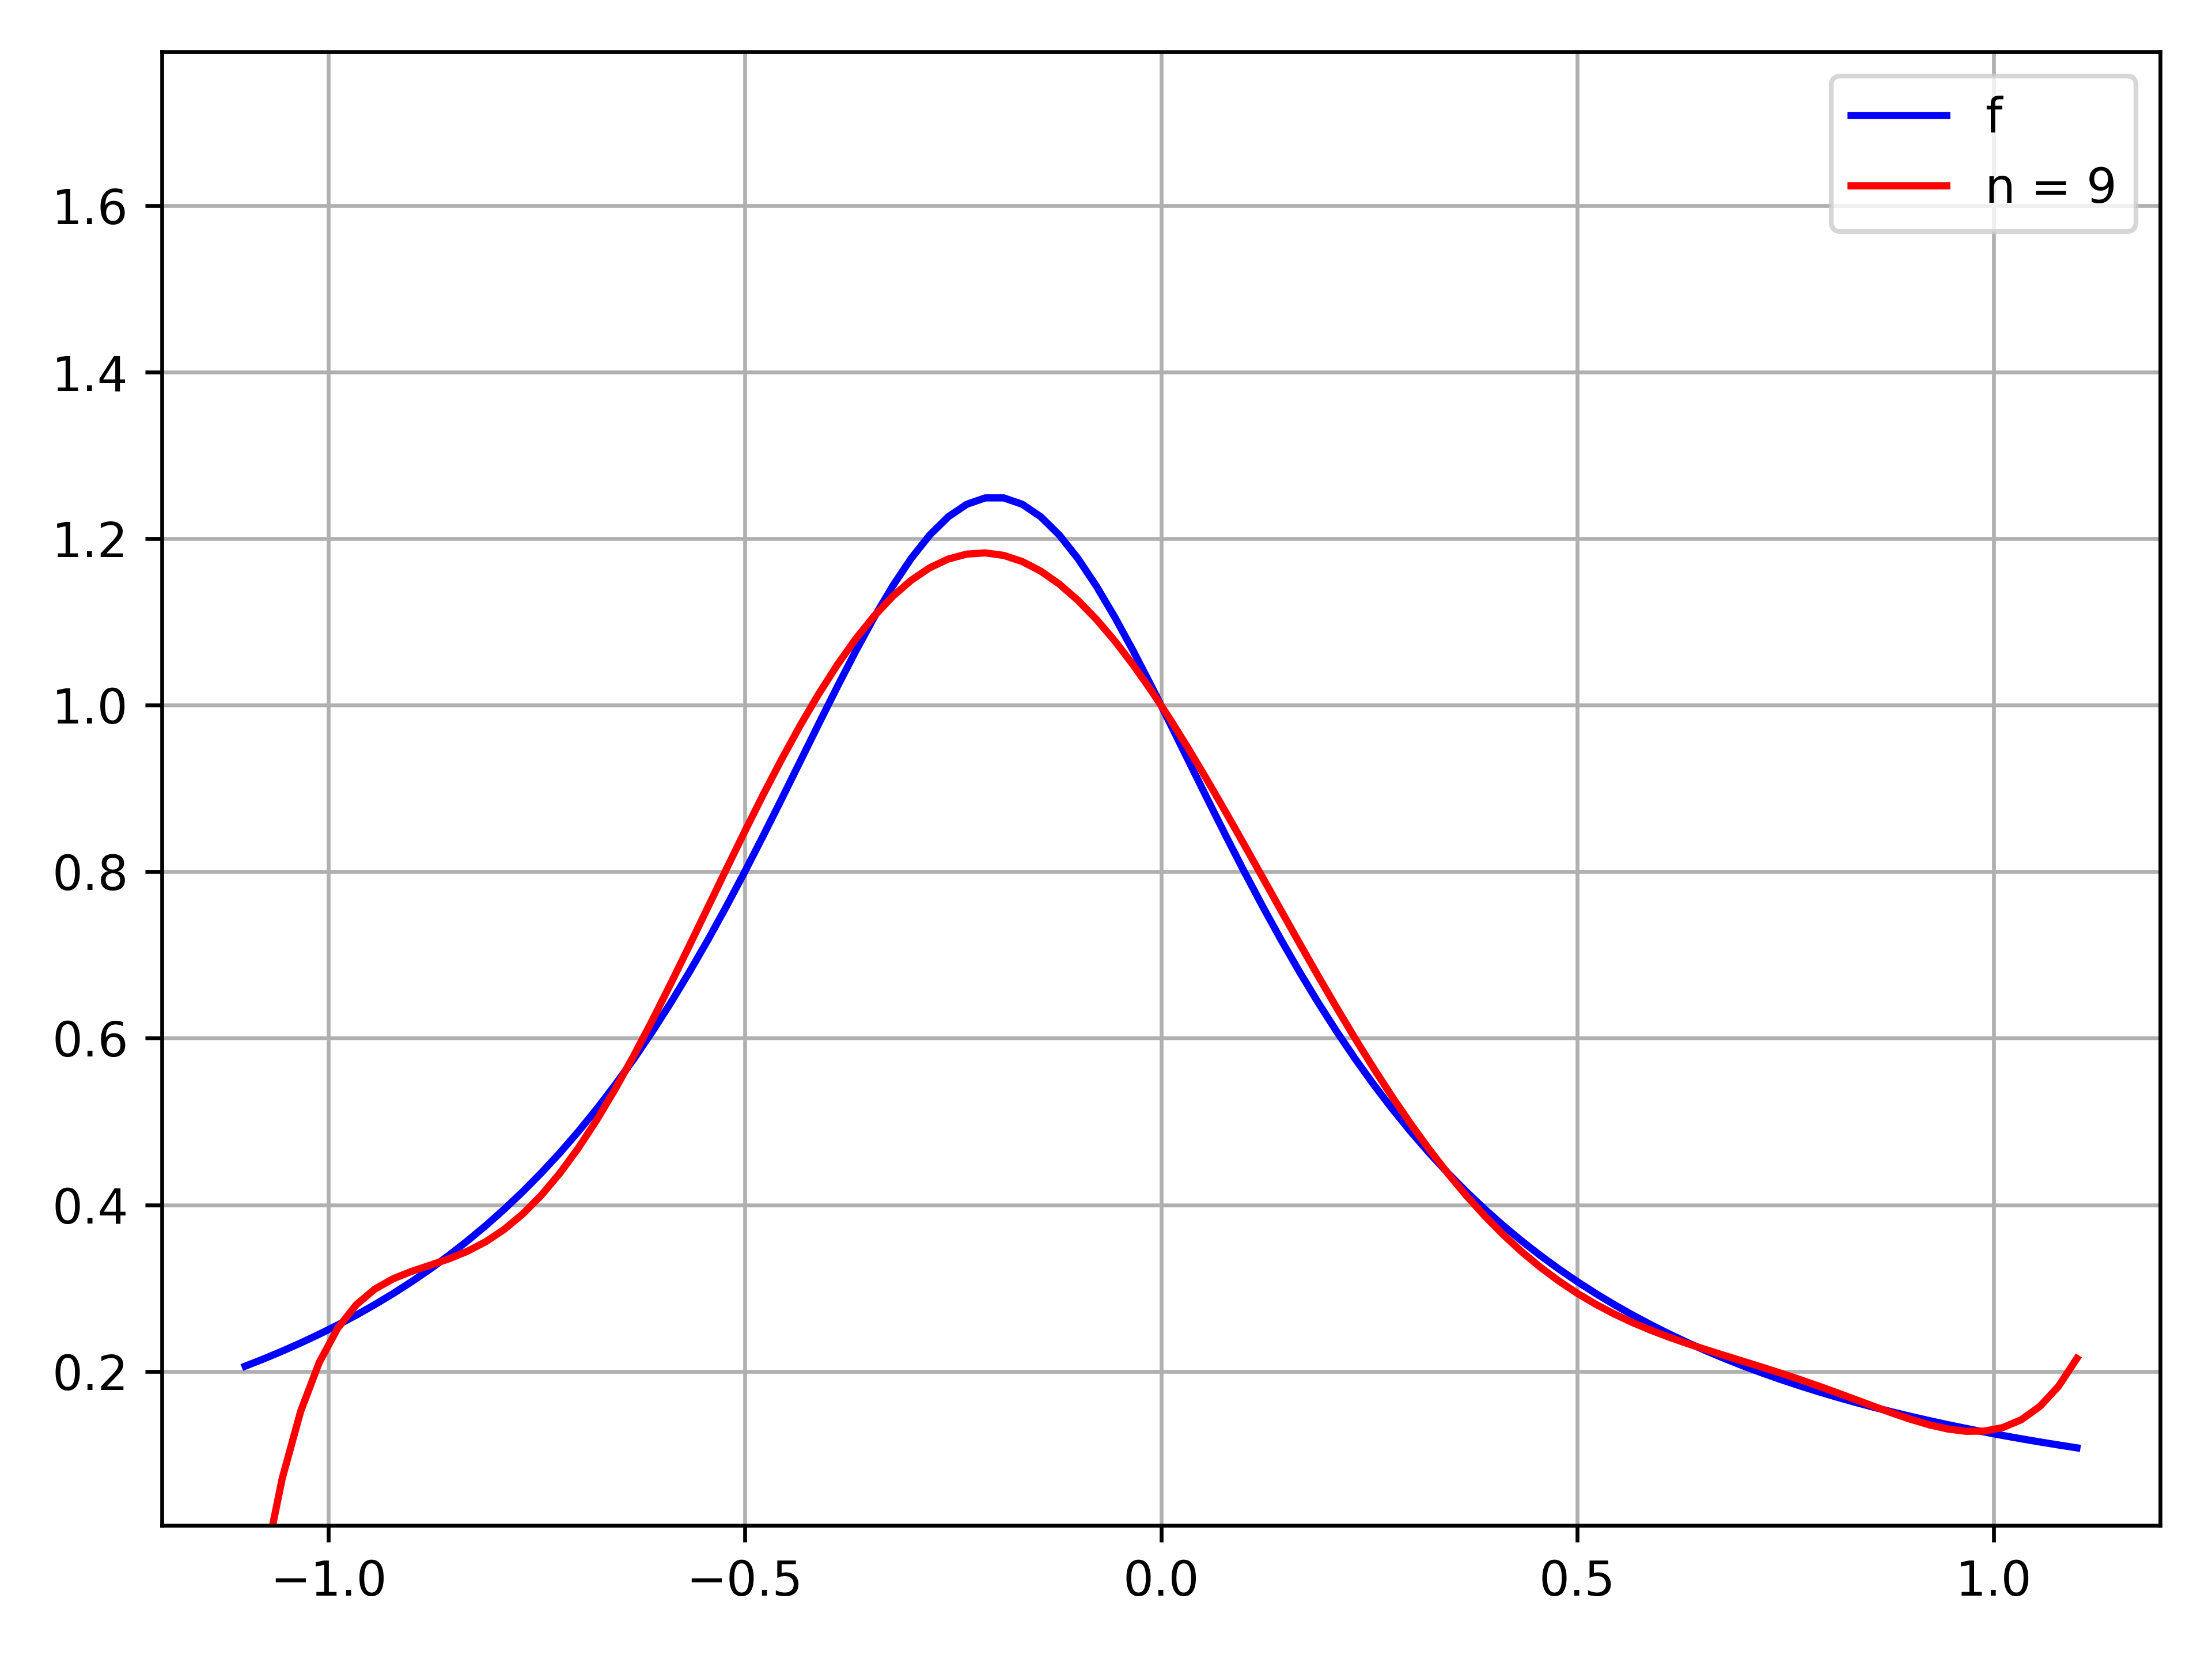
\includegraphics[scale=\myscale,scale=0.45]{figures/approx-tchebychev-03-9}
\end{center}
\end{exemple}

\begin{exemple}
On souhaite approcher $g(x) = \sin(x)$ sur l'intervalle $[0, \frac\pi2]$. 
On commence par transformer la fonction $g$ définie sur $[0, \frac\pi2]$ en une fonction 
$f$ définie sur $[-1,1]$ par :
$$f(x) = g\left( \frac{x+1}{2}\frac{\pi}{2}\right) = \sin\left( (x+1)\frac{\pi}{4} \right)$$
Calculons le développement en série de Tchebychev de $f$ pour $n=3$.
\begin{itemize}
  \item Tout d'abord, on rappelle :
$$T_0(X) = 1 \qquad T_1(X) = X \qquad T_2(X) = 2X^2-1 \qquad T_3(X) = 4X^3-3X$$

  \item Les racines de $T_3(X)$ sont :
$$
\omega_0 = \cos \left(\frac{1}{6}\pi\right) = \frac{\sqrt3}{2} \qquad 
\omega_1 = \cos \left(\frac{3}{6}\pi\right) = 0 \qquad 
\omega_2 = \cos \left(\frac{5}{6}\pi\right) = -\frac{\sqrt3}{2}
$$

  \item Les coefficients $c_i$ sont : 
$$c_0 = \frac{1}{3} \left( f(\omega_0) + f(\omega_1) + f(\omega_2) \right) 
\simeq 0.602202$$
$$c_1 = \frac{2}{3} \left( f(\omega_0) T_1(\omega_0) + f(\omega_1) T_1(\omega_1) + f(\omega_2) T_1(\omega_2) \right) 
\simeq 0.513518$$
$$c_2 = \frac{2}{3} \left( f(\omega_0) T_2(\omega_0) + f(\omega_1) T_2(\omega_1) + f(\omega_2) T_2(\omega_2) \right) 
\simeq -0.104905$$

  \item Ainsi le développement en série de Tchebychev de $f$ pour $n=3$ est :
$$f(x) \simeq P(x) = c_0 T_0(x) + c_1 T_1(x) + c_2 T_2(x)
= (c_0-c_2) + c_1 x +2c_2x^2$$

  \item Revenons à notre problème initial d'approcher $g(x) = \sin(x)$ sur l'intervalle $[0, \frac\pi2]$. On effectue la transformation inverse sur $P(X)$  
  $$Q(X) = P\left( \frac{4X}{\pi} -1 \right) $$


  \item Voici le graphe obtenu pour $Q(x)$ comparé avec celui de $g(x)$ (figure de gauche).
  L'erreur commise par cette approximation sur $[0, \frac\pi2]$ est partout inférieure à $0.02$ (figure de droite).

  \begin{center}
    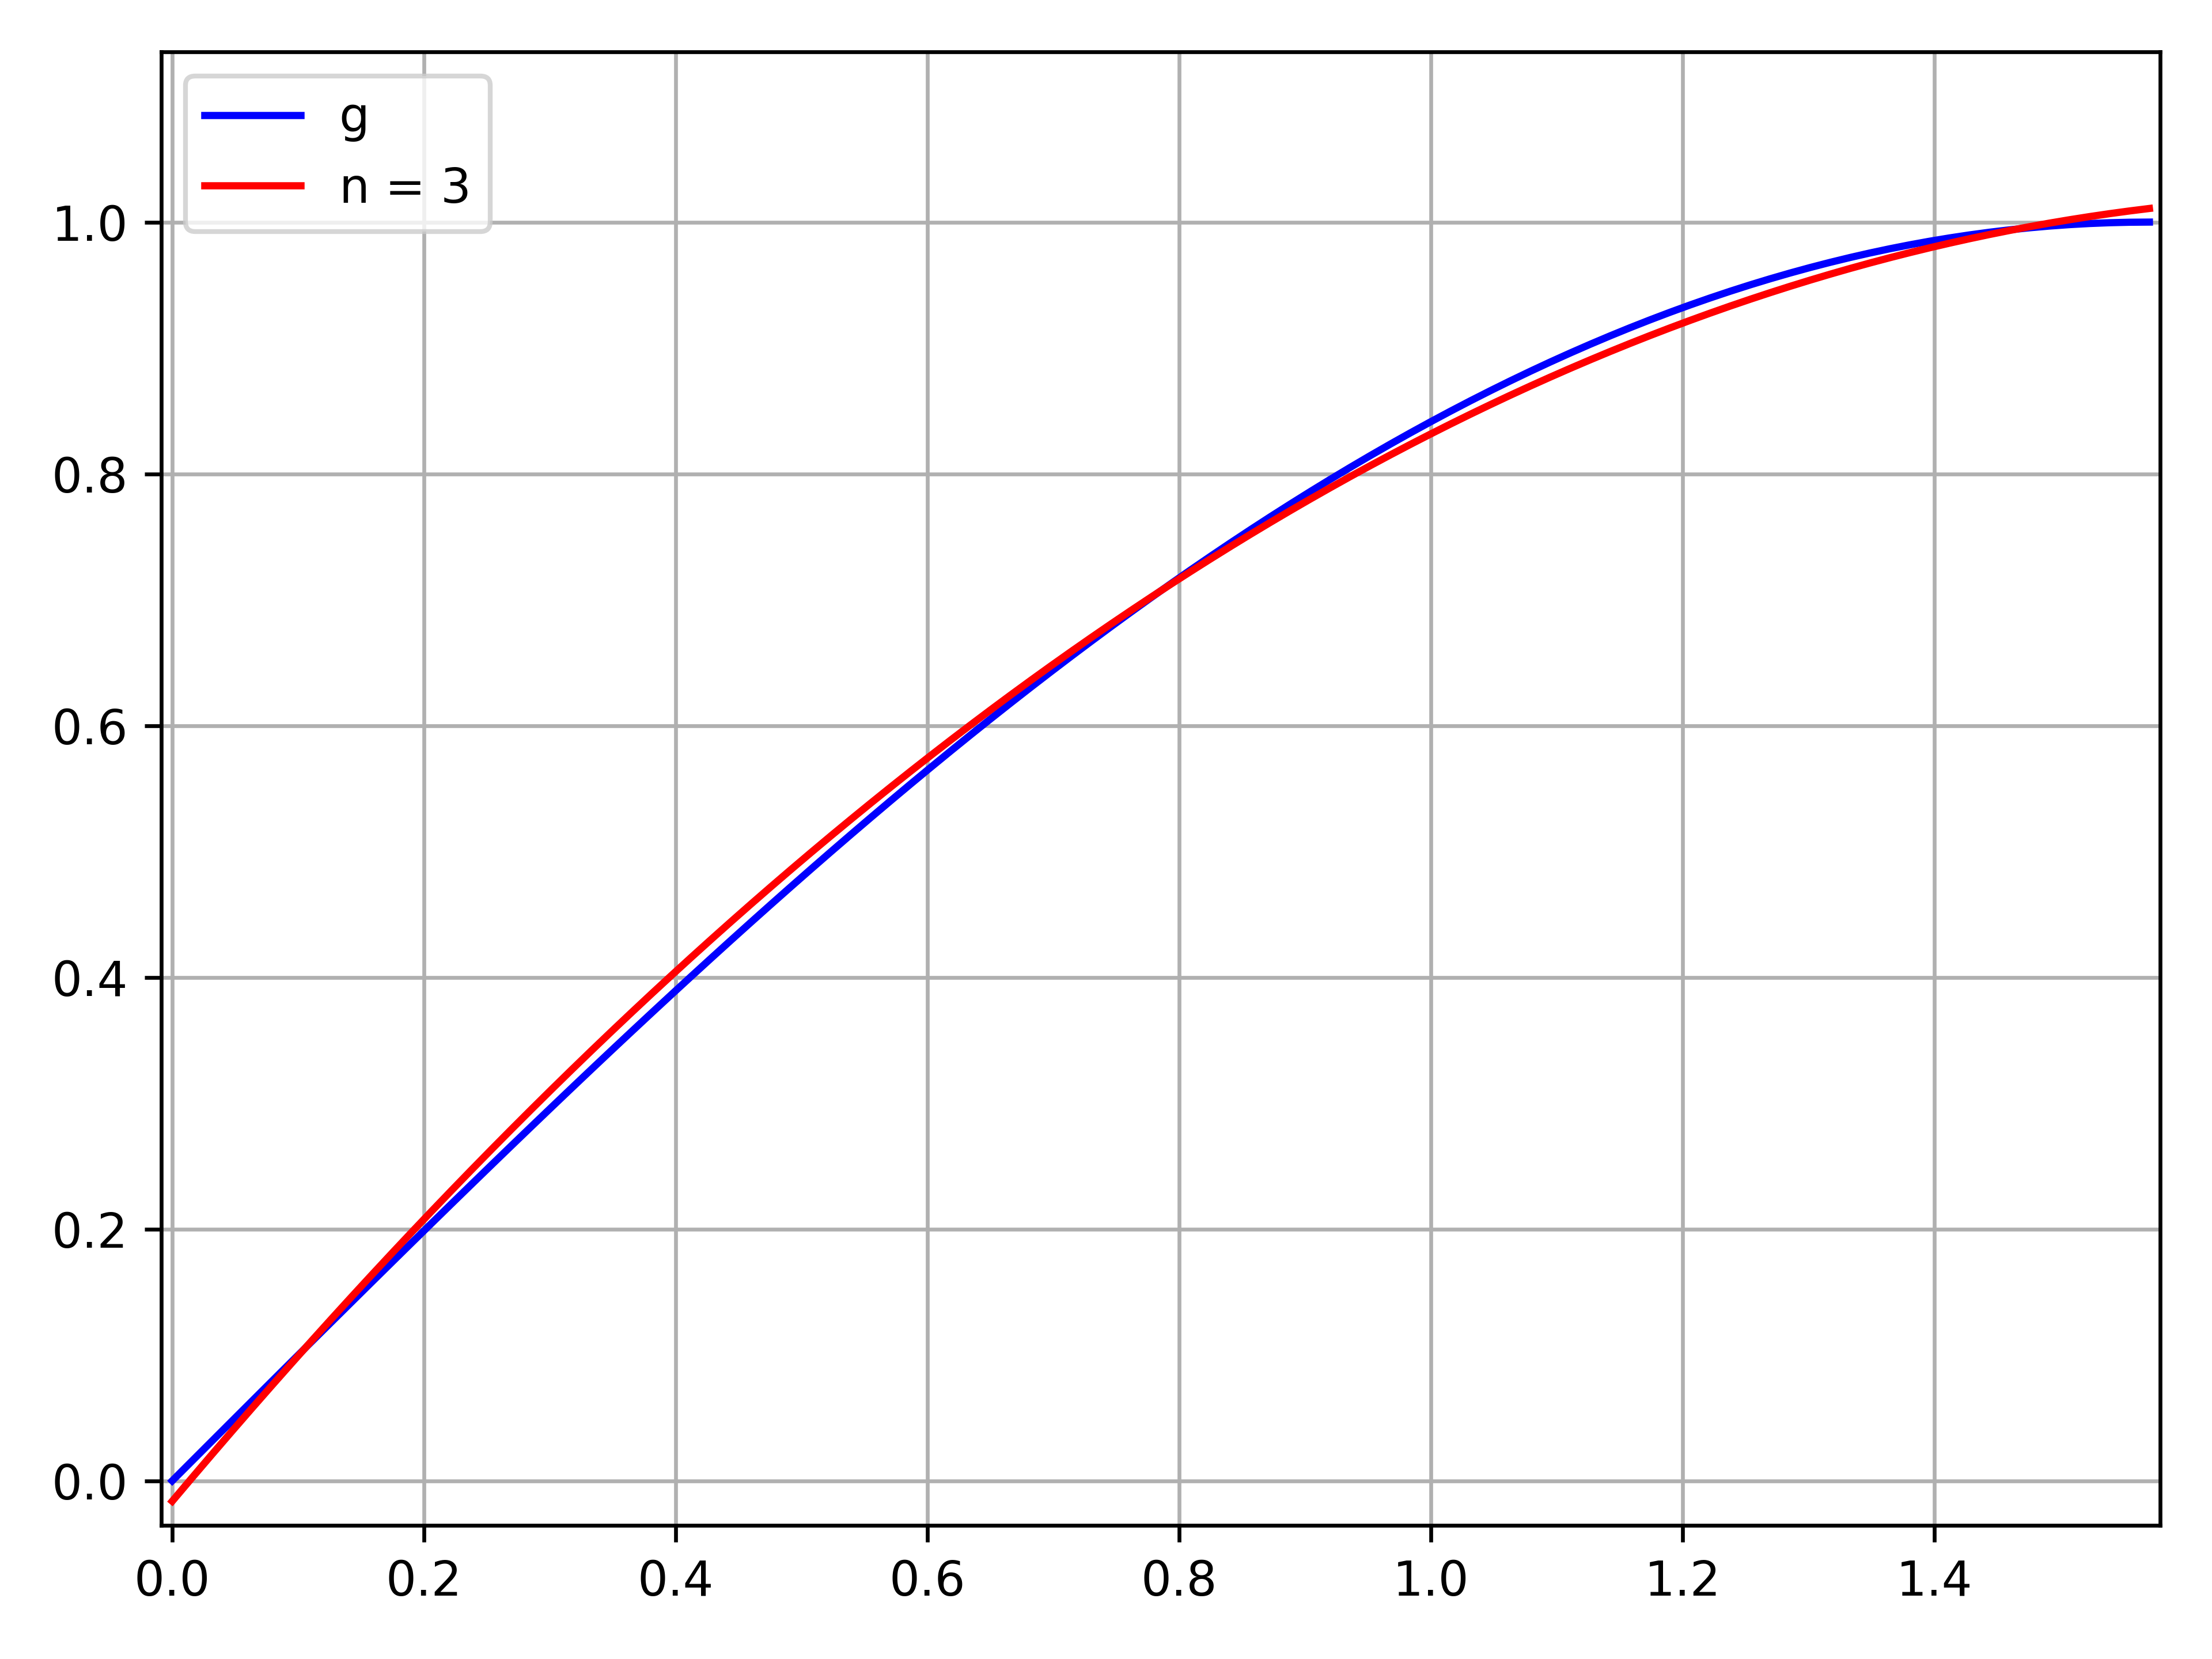
\includegraphics[scale=\myscale,scale=0.45]{figures/approx-tchebychev-04} \qquad
    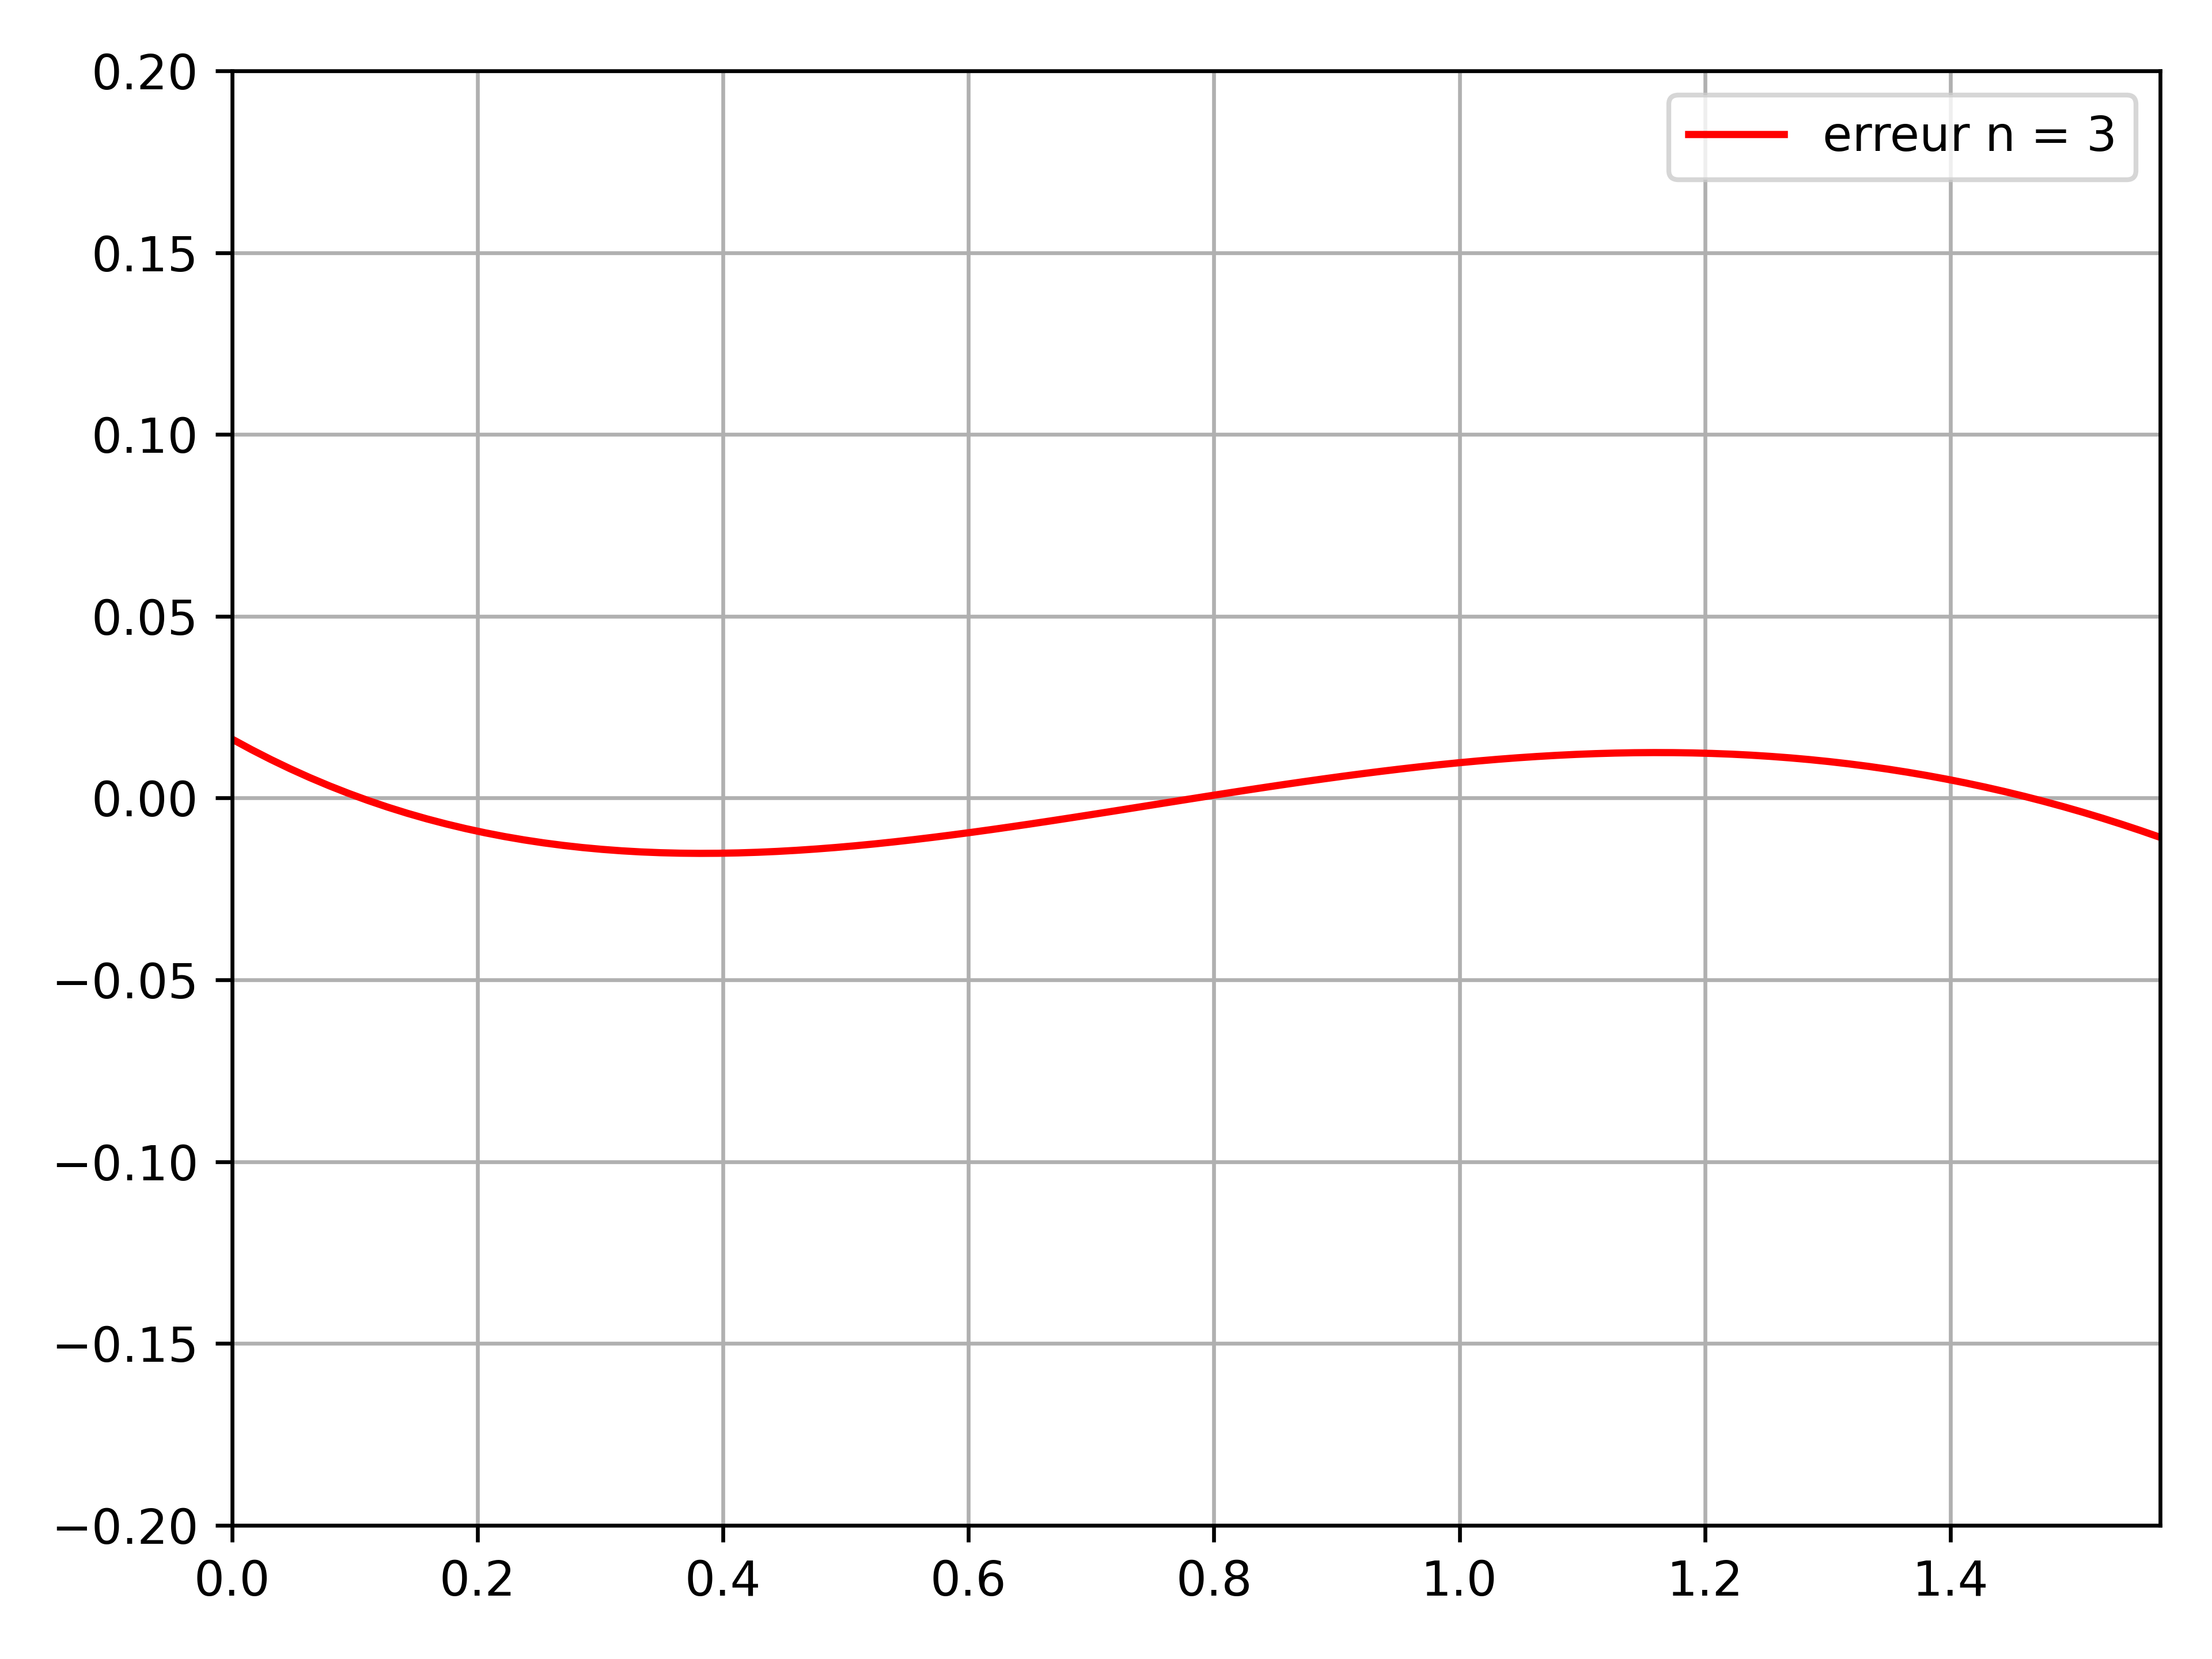
\includegraphics[scale=\myscale,scale=0.45]{figures/approx-tchebychev-05}
  \end{center}

\end{itemize}
\end{exemple}

%--------------------------------------------------------------------
\subsection{Approximants de Padé}

\index{approximation!de Pade@de Padé}

Au lieu d’approcher une fonction sur un intervalle par des polynômes on peut aussi l'approcher par des fractions rationnelles de la forme :
$$\frac{R(x)}{Q(X)} = \frac{a_0 + a_1 x + \cdots + a_n x^n}{b_0 + b_1 x + \cdots + b_m x^m}$$
où $R(x)$ et $Q(x)$ sont des polynômes de degrés respectifs $n$ et $m$.
Avec des polynômes de degrés plus petits on obtient une approximation équivalente à celle obtenue par un polynôme $P(X)$ de degré $n+m$.

\begin{exemple}
Soit $f(x) = \exp(x)$ à  approcher autour de $x_0=0$.
Le développement limité à l'ordre $4$ autour de $0$ est :
$$P(x) = 1 + x + \frac{x^2}{2} + \frac{x^3}{6} + \frac{x^4}{24}.$$

L'approximant de Padé de bidegré $(n,m) = (2,2)$ est :
$$\frac{R(x)}{Q(x)} = \frac{12 + 6x + x^2}{12 - 6x + x^2}.$$

Les comportements de $P(X)$ et de $\frac{R(x)}{Q(x)}$ autour de $x_0=0$ sont quasi-identiques mais les 
approximants de Padé peuvent avoir un comportement plus adapté loin de $x_0$.

\begin{center}
  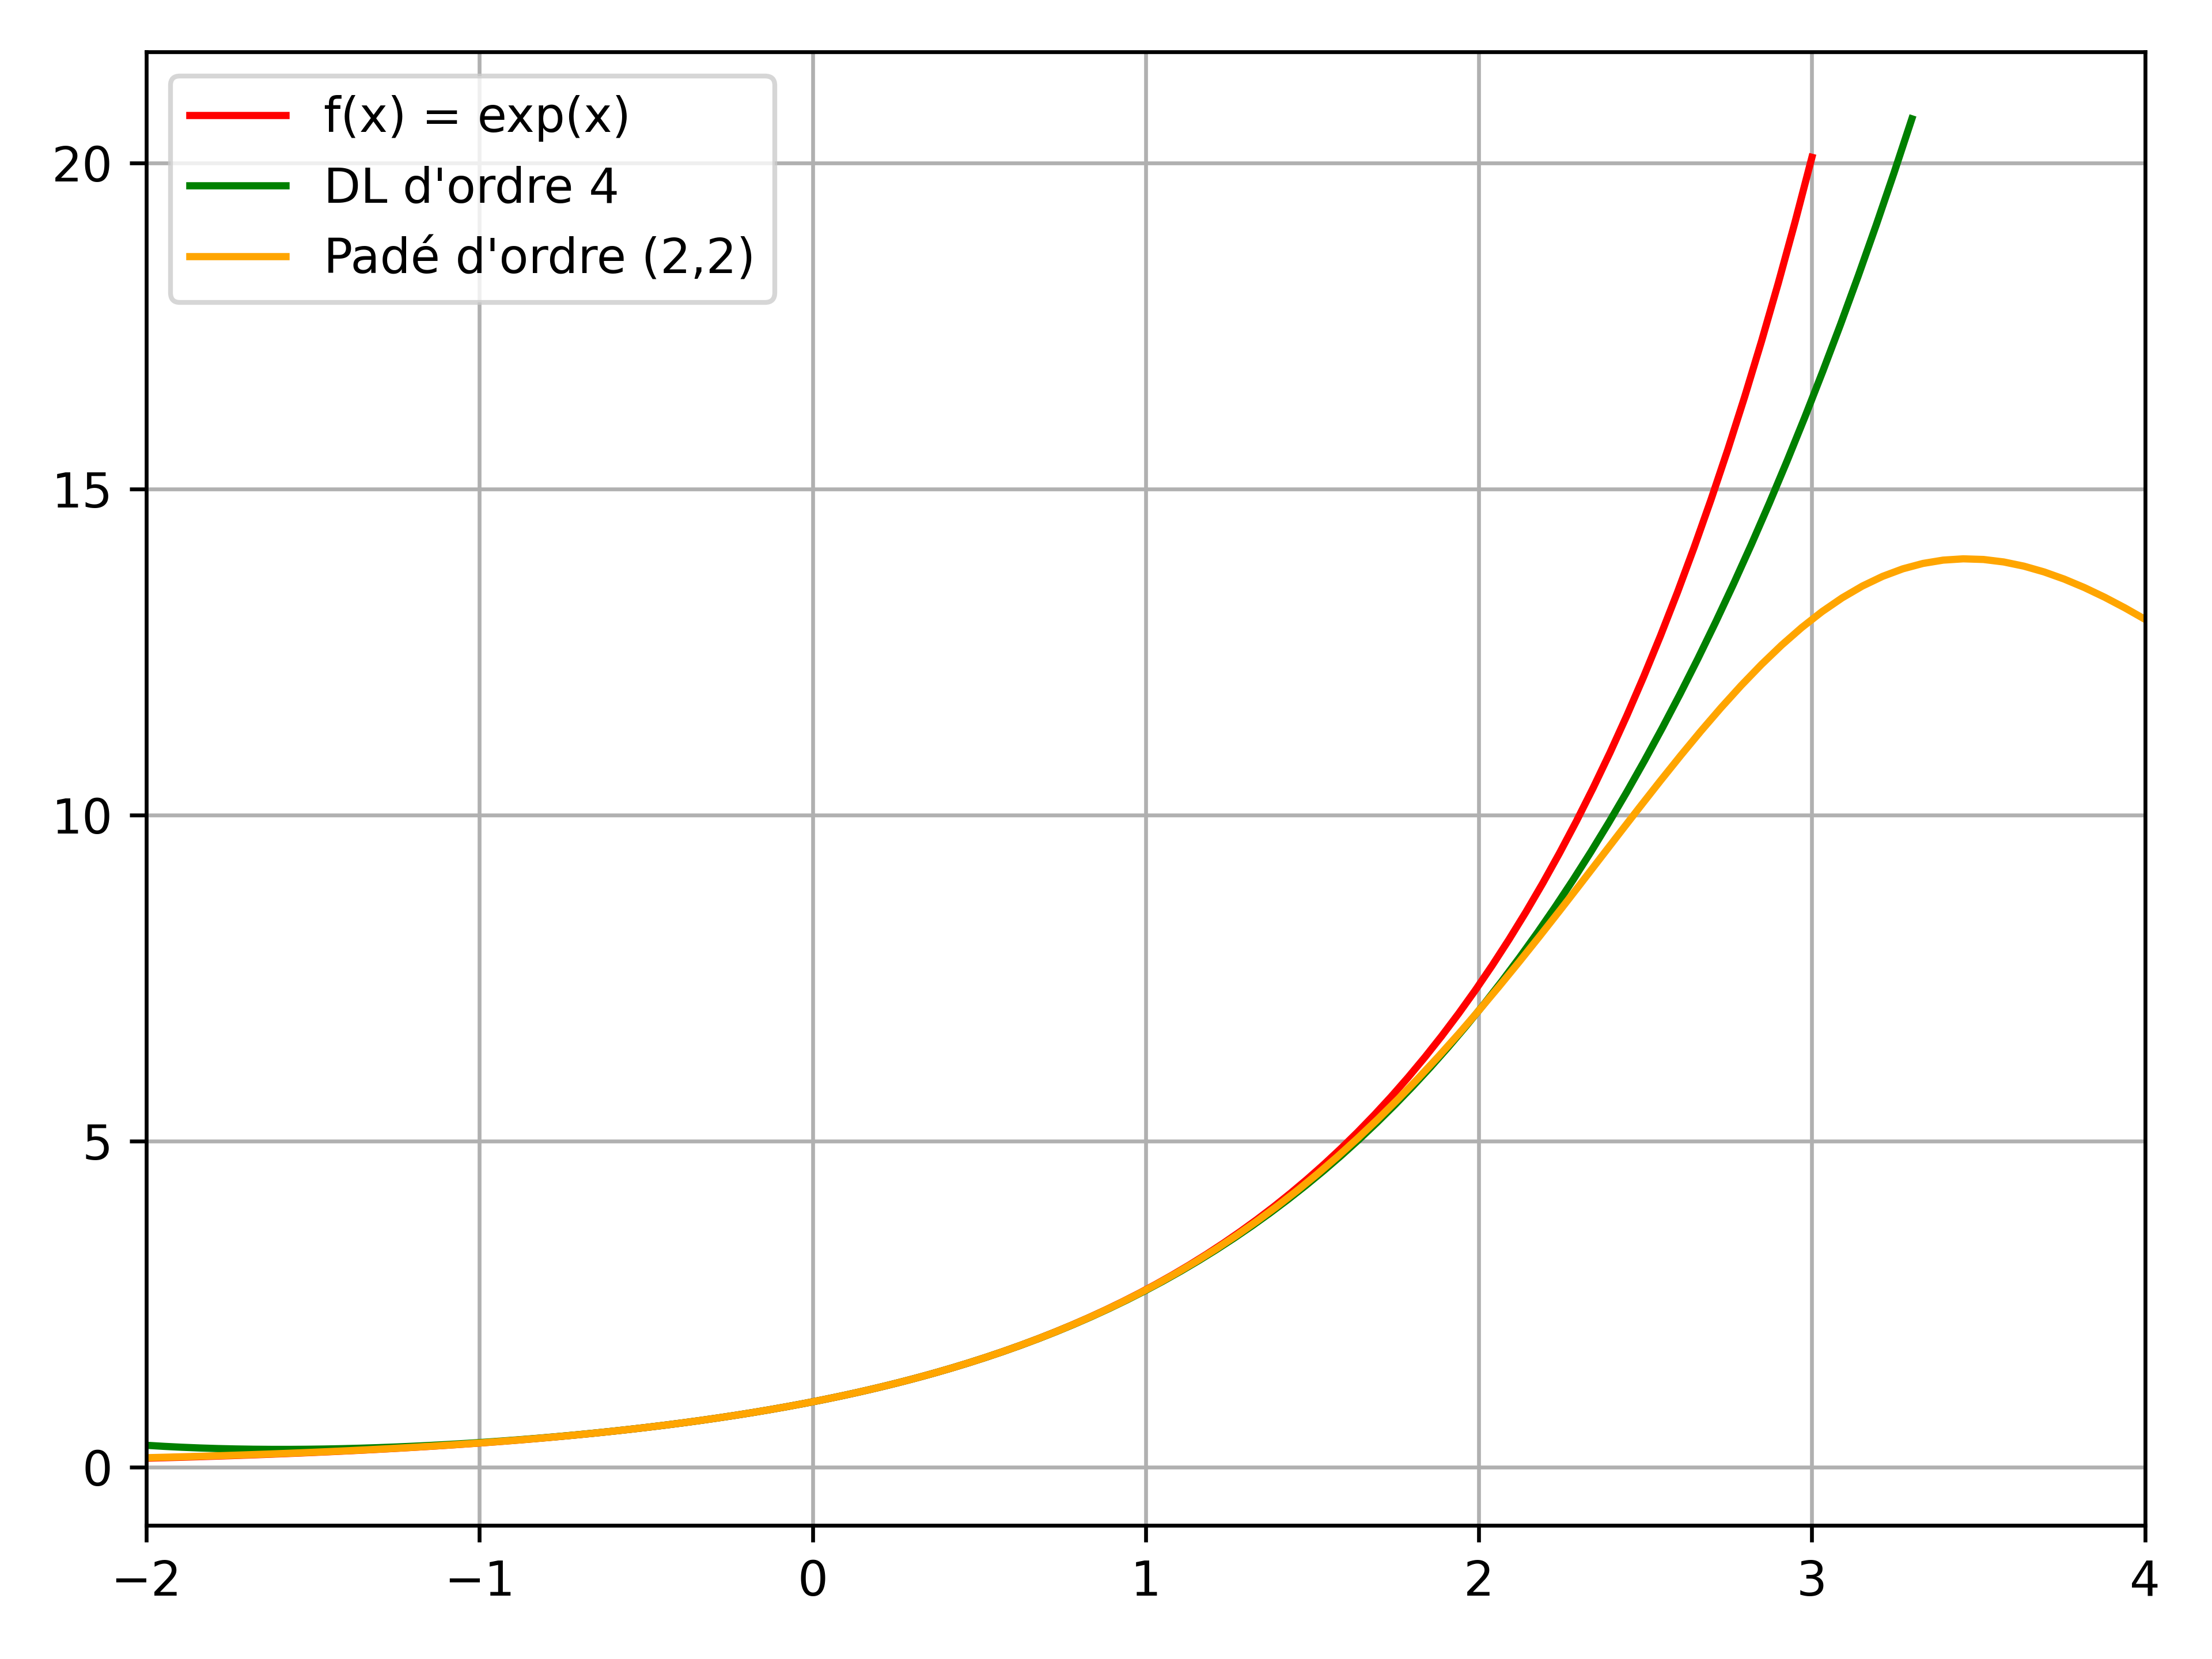
\includegraphics[scale=\myscale,scale=0.45]{figures/approx-pade-01} \qquad
  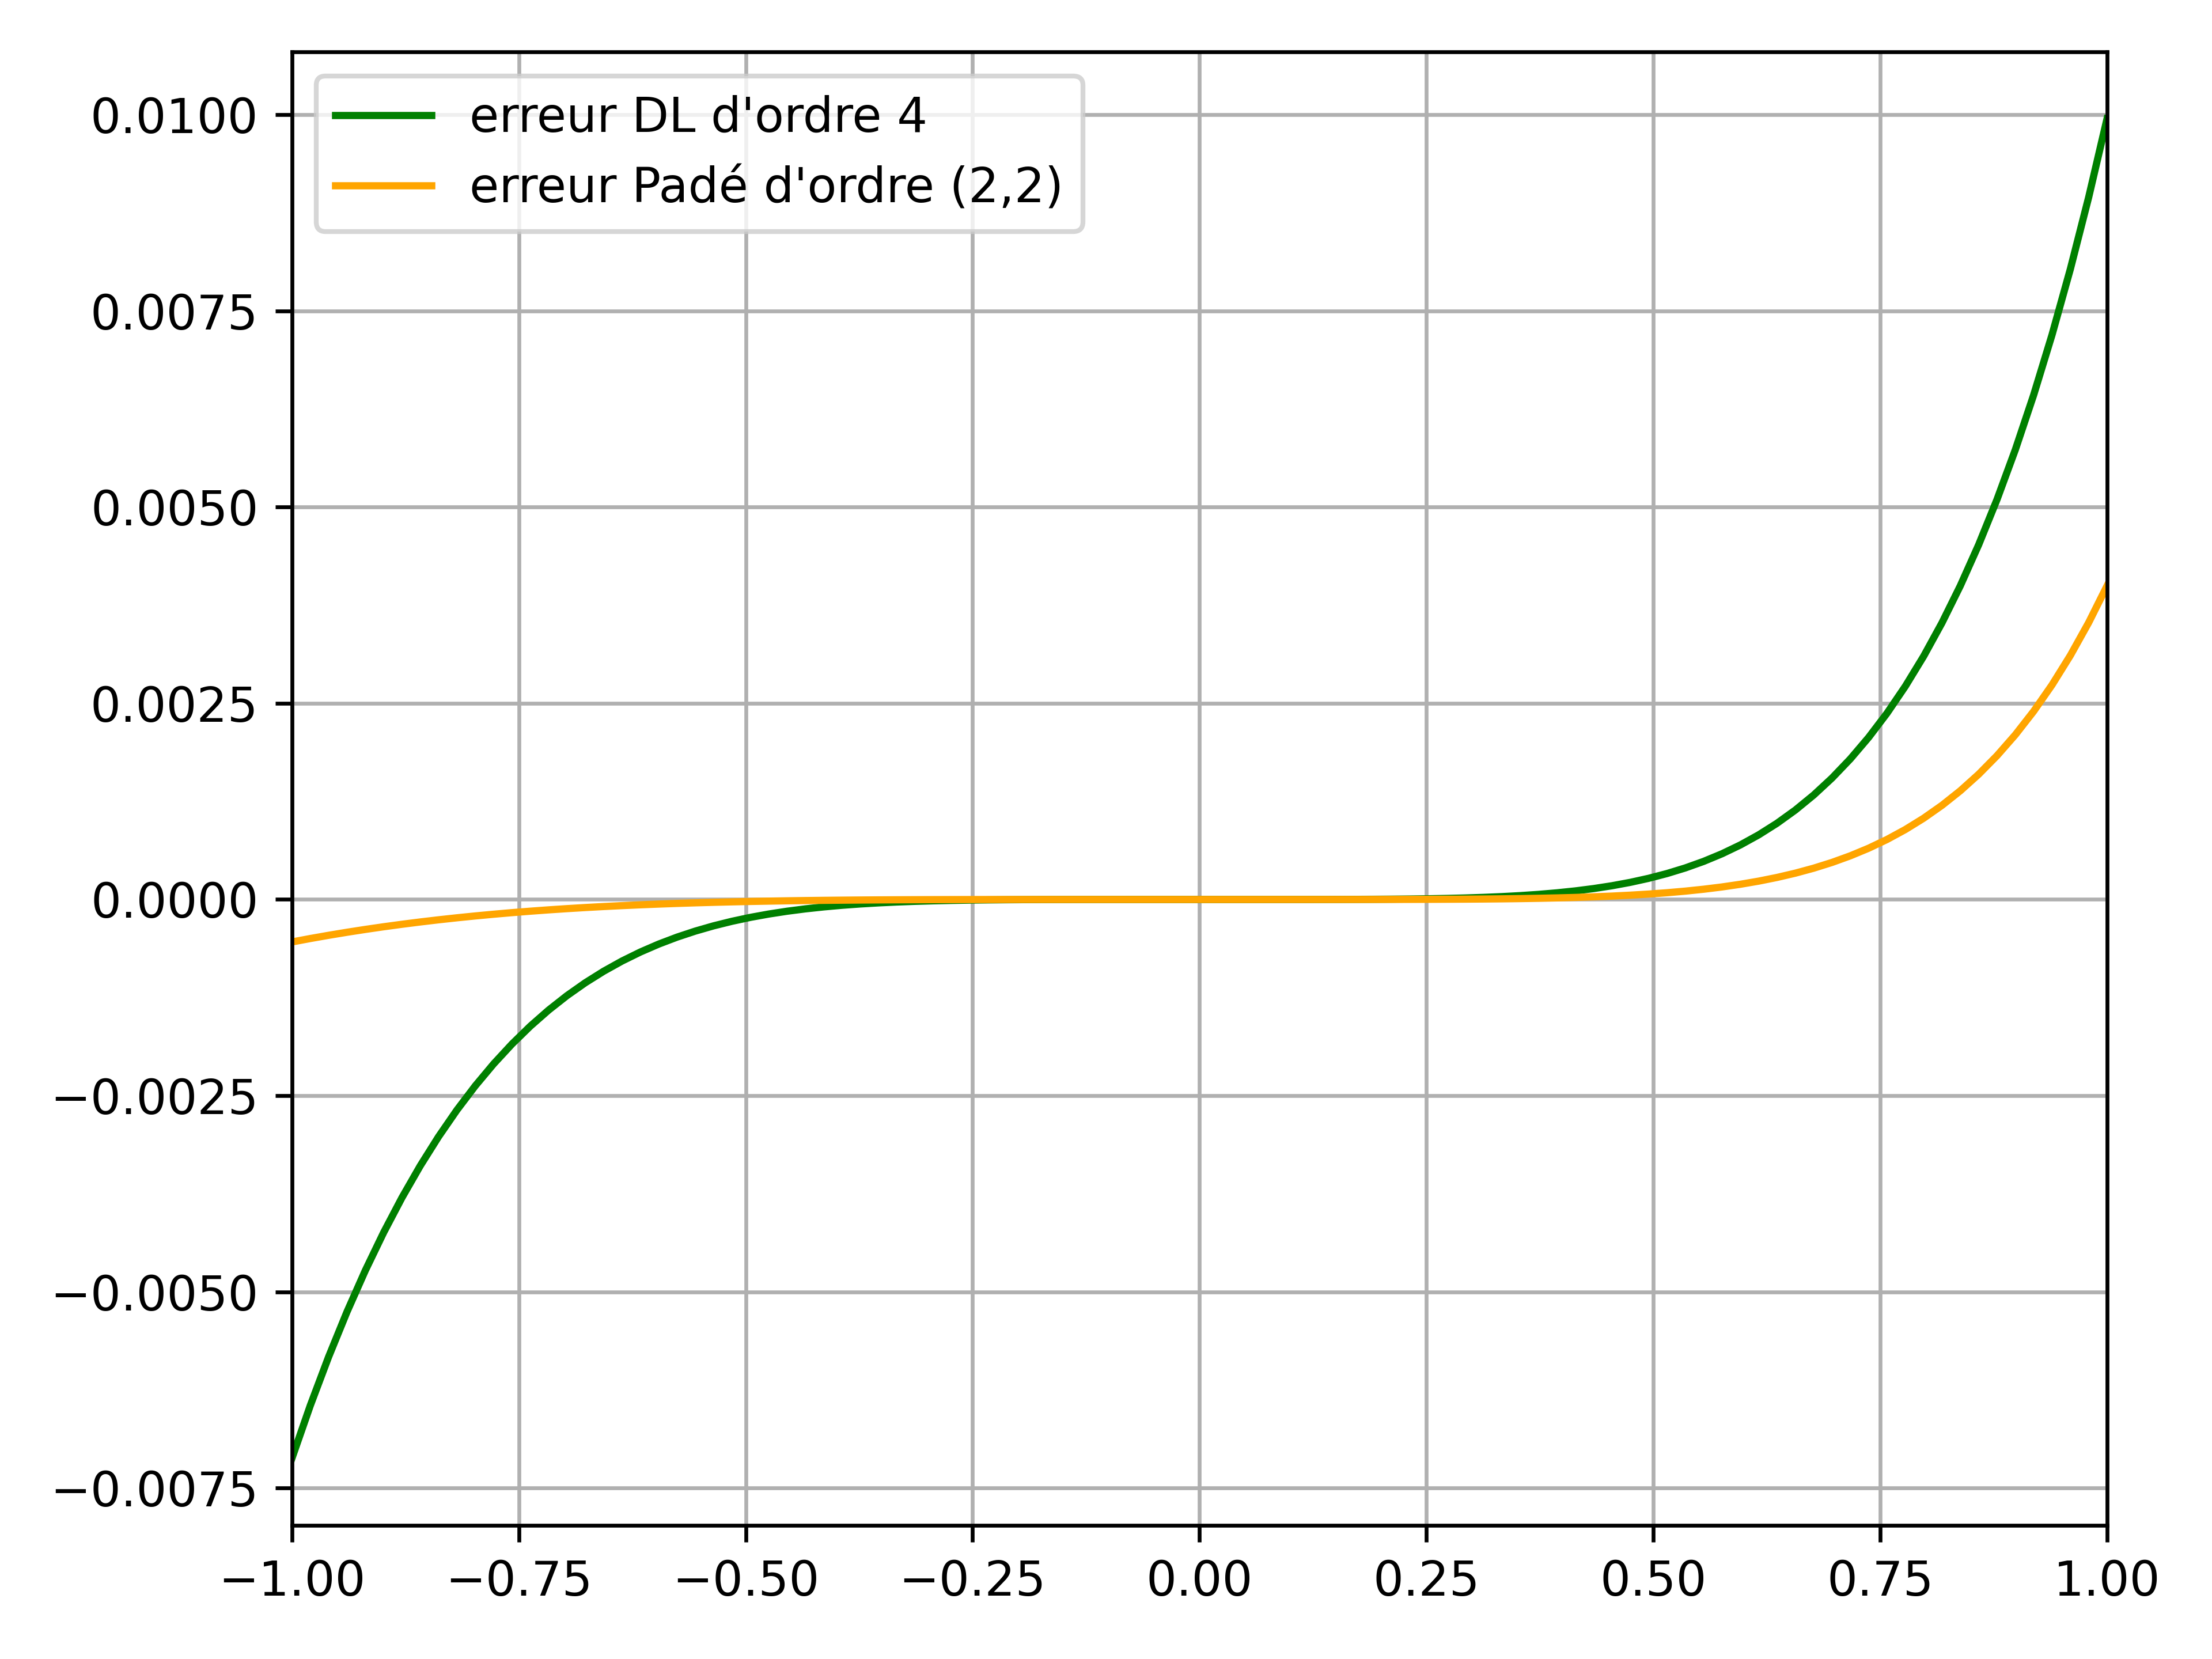
\includegraphics[scale=\myscale,scale=0.45]{figures/approx-pade-02} 
\end{center}

\end{exemple}




\end{document}